\documentclass[12pt,twoside]{report}
\usepackage[utf8]{inputenc}

\usepackage[a4paper,width=150mm,top=25mm,bottom=25mm]{geometry}

\usepackage{multirow}
\usepackage{graphicx}
\usepackage{color}
\usepackage{float}
\usepackage{amsfonts}
\usepackage{amsthm}
\usepackage{amsthm,amssymb,amsmath}
% \usepackage{multirow} % for tables
 \usepackage[english,british]{babel}
 \usepackage{textcomp}
%\usepackage{graphicx}
\usepackage{subfig}
\usepackage{hyperref}
\newtheorem{lemma}{Lemma}
\newtheorem*{remark}{Remark}


\usepackage[table,usenames,dvipsnames]{xcolor}

\usepackage{tikz}
%\usepackage{multirow}
\usetikzlibrary{shapes,arrows}
\usepackage{pdflscape}
\usepackage{rotating}

\usepackage{geometry}
 

\usepackage{xr-hyper} 
%\usepackage[colorlinks=true, pagebackref=true]{hyperref}

\RequirePackage{color}
\newcommand\red[1]{\textcolor{red}{#1}}
\newcommand\blue[1]{\textcolor{blue}{#1}}
\newcommand\green[1]{{\bf\textcolor{ForestGreen}{#1}}}
\definecolor{orange}{rgb}{0.7,0.3,0}
\newcommand\orange[1]{\textcolor{orange}{#1}}
\newcommand\mycol[1]{\textcolor{orange}{#1}}

\usepackage{longtable}
\setcounter{secnumdepth}{5}

\usepackage{fancyhdr}
%\pagestyle{fancy}


\usepackage[a4paper]{meta-donnees}

\Specialite{Physique pour les Sciences du Vivant}
\Arrete{7 août 2006}
\Auteur{Georgy Derevyanko}
\Directeur{Valentin GORDELY}
\CoDirecteur{Sergei GRUDININ}    %%optionnel : à décommenter et à renseigenr si présence d'un Co-directeur de thèse
\Laboratoire{Groupe des Transporteurs
Membranaires de l’Institut de Biologie Structurale}
\EcoleDoctorale{l'École doctorale de physique}         
\Titre{Structure-based algorithms for protein-protein interactions}
%\Soustitre{}      %%optionnel : à décommenter et à renseigenr si présence d'un sous-titre de thèse
\Depot{}       


% Commande pour création de nouvelles catégories dans le jury:

%\UGTNewJuryCategory{...NomDeLaCategorie...}{...Definition...}

% Exemple \UGTNewJuryCategory{UGTFamille}{Membre de la famille} que nous ajoutons dans la commande \Jury ci-dessous sous la forme \UGTFamille{Jean Rousseau}{(...titre_et_affiliation...s'il_y_en_a...)}


\Jury{
\UGTRapporteur{Martin ENGELHARD}{professeur, Max Planck Institut of Molecular Physiology}      %% 1er rapporteur
\UGTRapporteur{Georg BÜLDT}{professeur, Moscow Institute of Physics and Technology}      %% second rapporteur
 
\UGTExaminateur{Giuseppe ZACCAI}{professeur, Institut Laue-Langevin}     %% 1er examinateur
\UGTExaminateur{Grégory DURAND}{PhD, Maître de Conférences, Université d'Avignon et des Pays de Vaucluse }     %% second examinateur

\UGTDirecteur{Valentin GORDELIY}{professeur, Institut de Biologie Structurale}       %% Directeur de thèse
\UGTCoDirecteur{Sergei GRUDININ}{PhD Charge de Recherche, Inria Rhone-Alpes Research Center et Laboratoire Jean Kuntzman, CNRS}     %% Co-Directeur de thèse s'il y en a
}




\begin{document}
\MakeUGthesePDG    %% très important pour générer la couvérture de thèse



\chapter*{Abstract}
The phenotype of every known living organism is determined mainly by the complicated interactions between the proteins produced in this organism. Understanding
the orchestration of the organismal responses to the external or internal stimuli is based on the understanding of the interactions of individual proteins
and their complexes structures. The prediction of a complex of two or more proteins is the problem of the protein-protein docking field. Docking algorithms 
usually have two major steps: exhaustive 6D rigid-body search followed by the scoring. In this work we made contribution to both of these steps. 
We developed a novel algorithm for 6D exhaustive search, HermiteFit. It is based on Hermite decomposition of 3D functions into the Hermite basis. 
We implemented this algorithm in the program for fitting low-resolution electron density maps. We showed that it outperforms existing algorithms 
in terms of time-per-point while maintaining the same output model accuracy. We also developed a novel approach to computation of a scoring function, 
which is based on simple logical arguments and avoids an ambiguous com- putation of the reference state. We compared it to the existing scoring functions 
on the widely used protein-protein docking benchmarks. Finally, we developed an approach to include water-protein interactions into the scoring functions 
and val- idated our method during the Critical Assessement of Protein Interactions round 47. 

\chapter*{Dedication}
To my parents.

\chapter*{Acknowledgements}
I would like to thank my supervisor Valentin Gordely and co-supervisor Sergey Grudinin for their guidance during my thesis. I also thank my parents, brother and all the people
I was lucky to work with for their support.

\listoffigures 
\newpage
\listoftables
\newpage

\tableofcontents


\newpage
\chapter{Introduction}

  \section{Role of proteins and their interactions in the cell}
  The main dogma of biology states: information in a cell flows from DNA to RNA and then to proteins. Although the actual working of the cell is much more comlpex to be
contained in any dogma, it captures a large picture of the state-of-art of our understanding of the working of a cell. Proteins in this picture have a crucial place:
they are the cogs of the cell machinery. These are the protein expressed in a cell and their interactions that mainly define phenotype of that cell. Therefore gainig new 
data on the protein interaction in a cell profoundly enhances our capabilities to understand and change living organisms for the needs of the society.

\subsection{Classification of protein-protein interactions}
Commonly used classification of the protein-protein complexes uses the following main criteria: composition of a complex, its lifetime and stability \cite{nooren2003diversity}.

\subsubsection{Protein composition and interface}
The complex can be comprised of two identical or highly homologous proteins. An example of such a complex is the D-alanyl carrier protein (pdb code 4BPG), which consists of two identical
polypeptide chains (Fig. \ref{fig:exampleHomoDimer}). The proteins of this class are called homo-oligomers. On the other hand, if the complex consists of two distinct proteins it is named hetero-oligomer. 
An example of hetero-dimer (Glycosidase CelD bound to artificial affitin E12 protein, \cite{correa2014potent}, pdb code 4CJ0) is shown on Fig \ref{fig:exampleHeteroDimer}. 
Homo-oligomers are further divided dependent on the interface of oligomerization. If the two chains bind using the identical binding interace, their complex is called isologous. 
We can see that D-alanyl carrier protein is an example of isologous homodimer (Fig. \ref{fig:exampleHeteroDimer}). On the contrary, the homo-oligomeric assemblies where proteins bind through distinct
interfaces are called heterologous. 
%An example of the protein of this class is the abalone egg lysin dimer (pdb code 1LYN, \cite{shaw1995crystal}, Fig \ref{}). 
\begin{figure}[!ht]
\label{Fig:Step1Purification}
    \begin{minipage}{0.49\linewidth}
    \begin{centering}
      \includegraphics[width=1\linewidth]{Intro/Fig/HomoDimer.png}  
      \caption[Example of a homodimeric complex]{Example of a homodimeric complex,  D-alanyl carrier protein, pdb code 4BPG.}\label{fig:exampleHomoDimer}
    \end{centering}
    \end{minipage}
    \hfill
    \begin{minipage}{0.49\linewidth}
    \begin{centering}
      \includegraphics[width=1\linewidth]{Intro/Fig/HeteroDimer.png}  
      \caption[Example of a heterodimeric complex]{Example of a heterodimeric complex,  Glycosidase CelD bound to artificial affitin E12 protein, \cite{correa2014potent}, pdb code 4CJ0}\label{fig:exampleHeteroDimer}
    \end{centering}
    \end{minipage}
\end{figure}


\subsubsection{Stability of protomers}
The proteins that form a complex can be either stable or not on their own \emph{in vivo}. In the first case, when a complex is formed out of stable proteins it is called \emph{non-obligate}.
In many cases these proteins are localized in different compartements of a cell. Usually, interactions between receptor-ligand, enzyme-inhibitor, \emph{etc} belong to
non-obligate interactions. In the other case when a complex of one or both chains do not exist as folded proteins on their own, it is called \emph{obligate}.
An example of such a complex is the Arc repressor dimer, which consists of two peptide chains. Upon dimerization (catalized by DNA \cite{marcovitz2009arc}) these chains 
obtain stable secondary structure, that was absent in the monomer.

\subsubsection{Complex lifetime}
If two proteins form a very stable complex they said to interact \emph{permanently}. In many cases obligate complexes, such as Arc repressor dimer, are permanent.
On the other hand, if a complex is dissociated and formed continuously \emph{in vivo}, the interaction between its constituting proteins is called \emph{transient}. 
Many of non-obligate interactions are also transient. However, there are strong transient interactions that require the presense of some molecule for the complex 
dissociation. An example of a strong transient interaction is the formation of trimeric G protein, for which guanine triphosphate is the dissociation trigger.
  
  \newpage
  
  \section{Experimental methods to probe protein-protein interactions}
  Giving importance and variety of protein-protein interactions in a cell, numerous methods were developed to discover the fact that 
two or more proteins form a complex by measuring kinetics and free energy of its formation or even by solving the atomic structure of the complex.
The openness of the proteomics community also resulted in the construction of many databases of protein-protein interactions. All experimental methods of 
identification and characterization of protein-protein interactions
can be classified using two parameters: scale(high-throuput, individual) and system( \emph{in vivo}, \emph{in vitro}). Usually, a low-throuput approach
gives much more information about interaction properties, whereas a high-throuput one only identifies the presense or absense of an interaction.

\subsection{Yeast two-hybrid method (Y2H)}
The Y2H is probably the oldest and most widespread method to identify interaction of proteins \emph{in vivo}, which was scaled up to proteome level.
In the pioneering work by Fields S. and Song  O. \cite{fields1989novel} it was shown that if the domain of the transcription activator that directs 
binding to a promoter (BD) is separated from a domain that activates transcription from this promoter (AD), the transcription is deactivated.
Based on this principle, two proteins of interest are fused to BD and AD, respectively, and the transcription of the reporter gene signals if they interact (Fig \ref{Fig:Y2H}).

\begin{figure}[H]
    \begin{centering}
      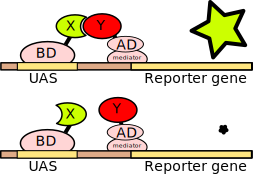
\includegraphics[width=0.5\linewidth]{Intro/Fig/Y2H.pdf}  
      \caption[Y2H explanation]{Schematic representation of the Y2H method. If the two protein X and Y do interact, expression of the reporter gene is high (yellow star), otherwise
      AD and BD domains of the promoter are separated and the expression is low. UAS stands for the upstream regulating sequence.}
      \label{Fig:Y2H}
    \end{centering}
\end{figure}

The are at least two scaling schemes: matrix and library approaches \cite{uetz2000comprehensive,ito2001comprehensive}. In the first one, 
clones expressing different proteins ${X_i}$ are taken and plated each
in the rows of wells on a plate. The same set of clones is plated in colums of wells on a plate. Then, when the two yeast cells in each well mate and make a diploid that
expresses both proteins $X_i$ and $X_j$. Afterwards, the expression of a reporter gene in a cell $i,j$ means that proteins $X_i$ and $X_j$ interact.
In the library-based approach, clones containig protein $X_i$ are screened agains a library of clones with various proteins, which can be expressed from
random cDNA or all open reading frames of a certain genome. In this case, the diploids expressing interacting proteins are selected agains specific growing media.
The proteins that interact with $X_i$ are determined by the DNA sequencing.

\subsection{Mass spectrometry and tandem affinity purification}
In this method, a certain protein is fused with the DNA sequence that expresses the TAP tag (IgG binding domains of \emph{Staphylococcus} protein A and calmodulin
binding peptide separated by the TEV protease site \cite{puig2001tandem}). When the DNA construct is expressed in a host, it produces the protein of interest that forms complexes
with other proteins of the host. During the purification, these protein complexes bind to the IgG matrix. Other proteins that did not form complexes with
the TAP-tagged one, hop through the matrix. Afterwards, using TEV protease, one cleaves of IgG binding domains and purified complexes are eluated from the matrix.
The second purification step is the binding to calmodulin-coated beads. The simple representation of the two-step purification is shown on Fig. \ref{Fig:TAP}.
Finally, the eluate is loaded to the SDS-PAGE gel and the resulting bands are cleaved by proteases.

After the purification, one uses mass-spectrometry to identify the fragments of the cleaved protein-protein complexes \cite{di2005molecular}. Mass-spectrometry identifies particles 
based on their charge-to-mass ration. It allows to recognize fingerprints of short peptides and therefore identify the proteins using the solution of 
peptide fragments.
A certain advantage of the TAP-MS method over Y2H is that it can detect not only dimeric protein-protein interaction, but also multimeric complexes.

\begin{figure}[H]
    \begin{centering}
      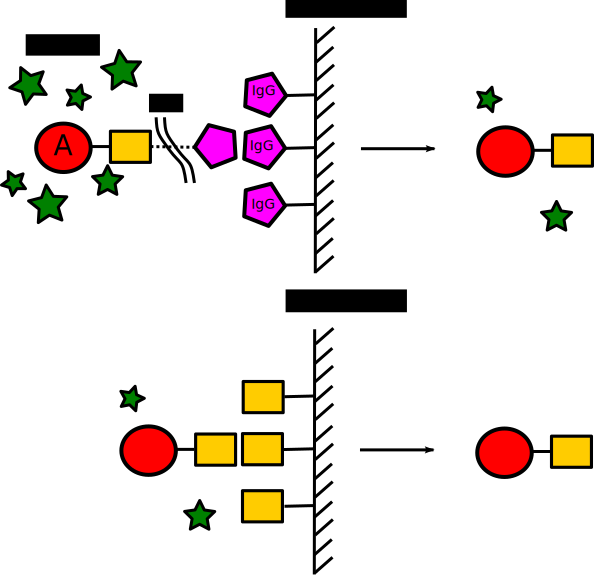
\includegraphics[width=0.5\linewidth]{Intro/Fig/TAP.pdf}  
      \caption[TAP-MS explanation]{Schematic representation of the tandem affinity pyrification method. Contaminants are shown with green stars, IgG binding domain is shown with 
      pink pentagon (as well as the IgG coating) and calmodulin (as well as calmodulin coating) is shown with squares.}
      \label{Fig:TAP}
    \end{centering}
\end{figure}

\subsection{Gene co-expression}
Recently the methods that allowed measuring expression of the genes on the scale of the whole cell were invented. Using this methodology,
one can measure the similarity of expression profiles over different conditions of the two or more genes that code for interacting proteins. 
It turns out that they are significantly more similar than the gene expression profiles of random non-interacting proteins \cite{jansen2002relating}.

\subsection{Synthetic lethality}
The mutations in the genome of an organism affect its phenotype. In many cases this phenotype alternation is caused by the change in the protein-protein interaction
network. By introducing random mutations or deletions in the genes of two proteins, one can monitor survival rate of these cells. The lethality of one such mutation 
can point to presence of interaction between the two target proteins \cite{ooi2006global}.

\subsection{Fluorescence resonance energy transfer}
The fluorescence resonance energy transfer (FRET) occurs between two molecules: one (donor) in an excited state and the orther (aceptor) in the ground state. 
The energy is transfered through the dipole-dipole interaction between the molecules and does not involve emission \cite{yan2003analysis}. The probability of such transfer to occur
strongly depends on the distance between the donor and the aceptor. However, it is almost independent of the environmental conditions, which makes this method a great
tool to study molecular interactions \emph{in vivo}. More specifically, the two fluorophores are fused to the two proteins of interest (Fig. \ref{Fig:FRET}). One is then excited using 
a laser and if these molecules form a complex, it transfers energy to the second fluorophore that emits light at a certain wavelength. One of examples
of FRET application is the investigation of membrane proteins dimerization \emph{in vivo}, in particular of melatonin receptor types 1A and 1B \cite{ayoub2004preferential}.

\begin{figure}[H]
    \begin{centering}
      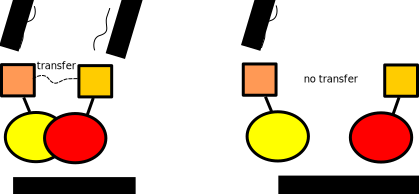
\includegraphics[width=0.5\linewidth]{Intro/Fig/FRET.pdf}  
      \caption[FRET explanation]{Schematic representation of the fluorescence resonance energy transfer method. If the two proteins interact, the fluorophores (blocks) come close and the energy
      transfer between them becomes possible. Therefore, exciting one fluorophore, one detects the emission from another. Otherwise, if the proteins do not interact,
      no emission of the second fluorophore is detected upon excitation of the first one.}
      \label{Fig:FRET}
    \end{centering}
\end{figure}

\subsection{Isothermal titration calorimetry}
This method allows to measure stoichiometry, dissociation constant, enthalpy and entrophy of the binding reaction between two proteins \cite{velazquez2005itc}. 
The experimental setup consists of two thermally isolated chambers.
One of the chambers is used as a reference and is filled with water. The other contains one of the interacting proteins. Its interaction partner is titrated in a known amount to the chamber. 
The thermometer measures temperature difference between these
two chambers and controls heaters to equilibrate their temperature (while maintaining the temperature of the reference chamber constant). 
The amount of heat spent to make the two chamber isothermic is measured during the experiment. 
Figure \ref{Fig:ITC} shows a schematic example of data obtained from an ITC experiment. The red line shows the peaks of energy transfer that correspond to titration events. Fitting 
these peaks with the interaction model (blue dashed line on Fig. \ref{Fig:ITC}) of a titration substance and a substance in the reservoir one can deduce the parameters of the model. 
In the simplest case of protein-ligand interaction one obtains enthalpy, dissociation constant and stoichiometry of the reaction.

\begin{figure}[H]
    \begin{centering}
      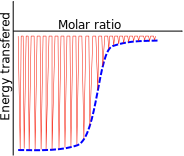
\includegraphics[width=0.5\linewidth]{Intro/Fig/ITC.pdf}  
      \caption[Isothermal titration calorimetry explanation]{Schematic representation of the data obtained from an isothermal titration calorimetry device. The red line 
      shows the energy transfered from the reservoir with the protein to the reference reservoir. Blue dashed line is an example of model fitted to the data.}
      \label{Fig:ITC}
    \end{centering}
\end{figure}

\subsection{Nuclear magnetic resonance spectroscopy (NMR)}
This method is based on the absorbtion and emission of radio-frequency radiation by the nuclei of certain atoms. The emission and absorbtion spectra depend on the 
environment of nuclei and therefore the measurement allows to reconstruct the distance matrix between certain atoms in a protein in solution. This method also
allows to measure the dynamics of proteins and their interaction. The classical approach is based on the Nuclear Overhauser Effect (NOE). One of the examples of the NMR results is
the structure of the Twist protein, a transcription factor that plays a key role in the epithelial-mesenchymal transition and the bromodomain-containing protein 4 \cite{shi2014disrupting} 
(see Fig. \ref{Fig:TwistBRD4}). Due to the complexity of spectra measured during the experiment, this approach is limited to protein complexes of the size up to 300 amino acids.

\begin{figure}[H]
    \begin{centering}
      \includegraphics[width=0.5\linewidth]{Intro/Fig/TwistBRD4.png}  
      \caption[The structure of Twist protein with the Brd4 protein]{The structure of Twist protein(green) with the bromodomain-containing protein 4 (red) measured using NOE-NMR technique \cite{shi2014disrupting}.
      PDB code 2MJV.}
      \label{Fig:TwistBRD4}
    \end{centering}
\end{figure}

\subsection{Cryo electron microscopy}
The broad variety of methods go under the name of Cryo electron microscopy (Cryo-EM). The basic principle underlying this method is the same as in the conventional
light microscopy. The difference lies in the radiation source. In Cryo-EM, the electron beam accelerated up to 300kV is used. This allows increasing the resolution that 
depends on the wavelength of the incident radiation, up to atomic one (wavelength of electrons accelerated by 300kV is about $0.02$\AA). However, the increased resolution
goes with the increased radiation dammage to the sample. Variety of methods are used to diminish ionizing effect of electrons on the biological samples. More precisely, 
measurement are conducted at low temperatures \cite{dubochet1988cryo}, averaging many identical units \cite{taylor1974electron}, single-particle microscopy.
The last one is probably the most used one in structural biology. 

The single-particle Cryo-EM is based on collecting information from many 2D projections of an object to reconstruct its 3D low-resolution model (electron density map, EDM). 
Afterwards, the supplementary information provided by NMR of X-Ray crystallography is used to construct an atomistic model of the object.

The 3D reconstruction of the EDM is usually based on the central projection theorem. It states that the Fourier images of 2D projections of a 3D object are the central slices of
its 3D Fourier images. The relative positioning of two projections can be derived from the common lines in their Fourier images. These algorithms
are implemented in the programs like IMAGIC \cite{van1996new}, SPIDER \cite{shaikh2008spider}, FREALIGN \cite{grigorieff2007frealign} \emph{etc}.

The resolution that can be obtained using this technique is highly dependent on the symmetry of the object measured. For example, highly symmetric icosahedral viruses 
envelopes were measured with up to 3\AA~ resolution \cite{zhang20103}. The other examples of reconstructed protein complexes usually have resolution in the range of 7\AA - 15\AA.
This method is the main source of information on the large protein-protein assemblies today, like ribosomes \cite{penczek2011identifying} and chperonines \cite{cong20104}.

\subsection{X-ray crystallography}
The X-ray crystallography is the most time- and cost- demanding method, but it provides the most detailed atomistic information on the structure of protein-protein 
complexes. The starting point of this technique is a protein crystal. Obtaining crystal of a certain protein-protein complex is often the major hurdle 
and sometimes even impossible. Large protein-protein complexes and membrane proteins are especially hard to crystallize. Nontheless, the X-ray crystallography 
remains a major method to study structures of protein-protein complexes. The method is based on the diffraction of X-rays on the atoms, arranged in a lattice.
The crystal of a protein is rotated with respect to the incident beam and the diffraction patterns are measured for each rotation. From these patterns
one can reconstruct the absolute values of the Fourier image of a unit cell of the crystal. Afterwards, the phases of the Fourier image have to be reconstructed
or measured. One of the most used way to obtain the phasing is the so-called molecular replacement. This means that approximate theoretical molecular structure of
the unit cell is fitted into the given dataset. Afterwards, one minimizes discrepancy of the fitted structure with the diffraction pattern and obtains the final one.
The quality of the final structure is judged by the R-factor. It shows to what extent the resulting structure explains the diffraction peaks.

  
  \newpage
  
  \section{Computational methods to probe protein-protein interactions}
  The experimental methods described in the previous section give rich information on the protein-protein interactions. However, in many cases
the interactions being identified using these techniques are incomplete and contradictory owing to certain limitations and biases of the
experimental conditions. To validate and cover the unknown spots in the protein-protein interactome maps, a plethora of computational
techniques is used. These methods rely on different assumptions and use different information sources to decipher interaction details 
of proteins. Despite the rich variety one can approximatelly classify them in two major groups: top-down methods that use whole-organism or even
evelutionary information and bottom-up, methods that employ the knowledge of single protein structures. They also differ by the amount of information
they provide: ranging from a simple fact of interaction down to the details and precise conformation of the interaction interface.

\subsection{Top-down approaches}
This class of methods use the evolutionary and genomic data to predict if two proteins interact and identify domains that contain the interaction interface.

\subsubsection{Gene neighbour and gene cluster methods}
This pack of methods rely on the assumption that genes encoding for possibly interacting proteins often transcribed as a single operon in procariotes
or co-regulated in eukariotes. A simplified example on how co-regulation maintains a certain stechiometry of a complex is shown on Fig. \ref{Fig:CoRegulation}.
For example, it was found that up to 75\% of co-regulated genes in bacterial and achaeal genomes interact \cite{dandekar1998conservation}.
The evolution tends to shuffle the order of genes in the distantly related organisms, however co-regulated gene clusters are found to be conserved. 
A prominent application of this method is the prediction of interaction of exsosome complex, that is capable of degrading viral RNA, and the RNAse P complex
by comparing the order of genes in archaeal and eukariotic genomes \cite{koonin2001prediction}.

\begin{figure}[H]
    \begin{centering}
      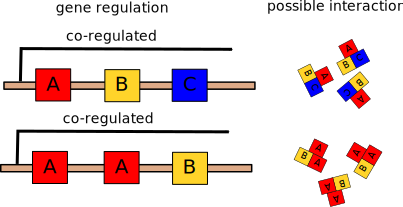
\includegraphics[width=0.5\linewidth]{Intro/Fig/CoRegulation.pdf}  
      \caption[Co-regulation scheme]{Example of a gene co-regulated cluster and the probable complex with the stechiometry set by the co-regulation.}
      \label{Fig:CoRegulation}
    \end{centering}
\end{figure}

\subsubsection{Phylogenetic profile methods}
These methods are based on the hypothesis that the interacting proteins coevolve and therefore have orthologous proteins among sequenced organisms \cite{barker2005predicting}.
If the proteins related to the two proteins in question are present in majority of organisms therefore, they probably constitute 
a pathway or physically interact. The phylogenetic profiles are constructed for the proteins where their presense indicated by 1 or 0. Then, these
profiles are clustered and the proteins belonging to one cluster are assumed functionally related or interacting.

\subsubsection{Rosetta Stone method}
This method relies on the observation that interacting proteins have homologs in other organisms that are fused into one protein. These types of proteins
are called Rosetta Stone proteins. This fusion is the limiting case of the co-expression optimization of functionally related proteins. Using this method
Marcotte \emph{et all} \cite{marcotte1999detecting} identified about 7,000 pair of potentially interacting proteins in \emph{E.Coli} and further analysis of the data revealed
that around a half of these pairs are functionally related.

\subsubsection{Co-evolution based methods}
During the evolution, mutations in one of the proteins of a complex should be compensated by the mutations in its partner in order to maintain the function (see Fig.\ref{Fig:CoEvolution}). 
The co-evolution based methods use the similarity measures between phylogenetic trees of two interacting protein families. Studies showed that some implementations 
of this method can predict up to 50\% of real interactions with false positive rate as low as 6.4\% \cite{pazos2001similarity}.

\begin{figure}[H]
    \begin{centering}
      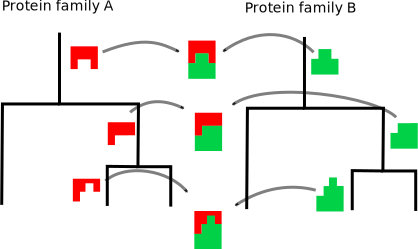
\includegraphics[width=0.5\linewidth]{Intro/Fig/CoEvolution.pdf}  
      \caption[Co-evolution scheme]{Example of a genes co-evolution where evolutionary changes in one protein compensate for the changes in its interaction partner.}
      \label{Fig:CoEvolution}
    \end{centering}
\end{figure}

\subsection{Bottom-up approaches}
Bottom-up approaches to the prediction of protein-prtoein interactions rely on the known structure of the proteins that constitute the complex.
The structures can either be modelled by homology, obtained using evolutionary constraints or taken from such experiments as NMR, X-Ray crystallography
or Cryo-EM. These methods are usually applied to infer the missing structural information about the protein-protein complex rather than to predict the fact
of interaction. 
Because bottom-up approaches use two or more protein structures that they dock into a complex, this class of techniques are usually called docking algorithms.
The pioneering work in this field was done by Janin and Wodak \cite{wodak1978computer}. Since then, this field has grown enormously, with its own
 quality assessment \cite{Mendez2003,Mendez2005,Janin2009}.
The two major parts of all the algorithms in this field are: sampling and scoring \cite{ritchie2008recent, huang2014search}. As the name suggest, the sampling part 
generates putative conformations of a complex of proteins and scoring ranks them according to some criteria. 

\subsubsection{Search strategies}
Suppose we have two molecules that are assumed to be rigid. One of the molecules (usually the one of a higher molecular weight) is called receptor and is fixed at the origin of the coordinate frame.
The other, called ligand, is moved around the receptor. The global search algorithm explores all possible rotations and translations of the ligand movements.
Complexity of this problem is $O(N^9)$, where $O(N^3)$ comes from rotational, $O(N^3)$ from the translational degrees of freedom and $O(N^3)$ is the complexity of the 
integration of the overlap integral that is computed for each rotation and translation of the ligand. A rough estimate
gives $\approx 10^{10}$\cite{huang2014search} operations. Several approaches allowed reducing this enormous complexity by at least an order of magitude.
These are the fast Fourier transform correlation and clever heuristics in the direct search.

\paragraph{FFT-based rigid body docking}
The idea to perform correlations in the Fourier space was first used by Katchalski-Katzir and colleagues \cite{katchalski1992molecular}. 
In this section I give a short description of this approach with a comprehesive 2D example.

Suppose that proteins receptor ($\mathbf{R}$) and ligand ($\mathbf{L}$) are represented as the numbers on a 3D grid:
\begin{eqnarray}
 R(l,m,n)= \begin{cases}
            1, (l,m,n)\in \mbox{surface of }\mathbf{R}\\
            \rho, (l,m,n)\in \mbox{inside of }\mathbf{R}\\
            0, (l,m,n)\in \mbox{outside of }\mathbf{R}
           \end{cases}
L(l,m,n)= \begin{cases}
            1, (l,m,n)\in \mbox{surface of }\mathbf{L}\\
            \delta, (l,m,n)\in \mbox{inside of }\mathbf{L}\\
            0, (l,m,n)\in \mbox{outside of }\mathbf{L}
           \end{cases}
           \label{Eq:LigRecGrid}
\end{eqnarray}
where $\rho\ll-1$ and $0<\delta<1$, according to the original work by Katchalski-Katzir \cite{katchalski1992molecular}. The shape complementarity score will therefore read:
\begin{equation}
 C(p,q,r)=\sum_{l,m,n=1}^{N} R(l,m,n)\times L(l+p,m+q,n+r),
\end{equation}
where the periodic boundary conditions are applied. Function $C$ defined on the same grid gives complementarity score that depends on the shift of the ligand $(p,q,r)$.
This function can be computed using the FFT algorithm as follows:
\begin{equation*}
 C(p,q,r)=\mbox{FFT}^{-1}\left[ \overline{\mbox{FFT}[\mathbf{R}]}\times \mbox{FFT}[\mathbf{L}]\right], \label{Eq:FFTDockingConvolution}
\end{equation*}
where $\mbox{FFT}^{-1}$ stands for the inverse fast Fourier transform and overline for the complex conjugate. This algorithm allows to rapidly sample translational degrees of freedom.
The rotations of the protein are separated from the translations in the outer loop of the algorithm. Fig. \ref{Fig:FFTDocking} shows a comprehensible example of 2D calculations
using this approach.

An example of the docking procedure is shown on Fig. \ref{Fig:FFTDocking}. The first row shows the picture of receptor and its Fourier image. The first column shows different
ligand poses. The border outlined with the dark-blue and the inner space with light-blue. The numbers placed on the grid are described by Eq. \ref{Eq:LigRecGrid}.
The second column shows the Fourier images of receptor and individual ligand poses. Third column shows the phases of Fourier image of the convolution 
$\mbox{FFT}[C(p,q,r)]=\overline{\mbox{FFT}[\mathbf{R}]}\times \mbox{FFT}[\mathbf{L}]$. The phases of the inverse Fourier transform of the data from the third column are
shown in the fourth one, it was computed according to Eq. \ref{Eq:FFTDockingConvolution}. Finally, in the last column the pose with the best score is shown, here the ligand is shown with the light-blue and the 
receptor is depicted with the dark-blue color. The images of Fourier transforms were built using the projection of complex values to the HSV colorspace \cite{PetrisonE2013visualizing} with the 
amplitude fixed to $V=100.0$.

\begin{figure}[H]
    \begin{centering}
      \includegraphics[width=1.0\linewidth]{Intro/Fig/DockingExample}  
      \caption[FFT-based docking example]{Example of a FFT-based docking procedure.}
      \label{Fig:FFTDocking}
    \end{centering}
\end{figure}


%In the modern algorithms based on the idea described above, a simple shape complementarity is usually coupled to the information about binding site  \cite{eben2003weighted}, 
%electrostatic energy \cite{gabb1997modelling}, atomic desolvation effect \cite{chen2002docking}, 
%knowledge-based potentials \cite{mintseris2007integrating}, \emph{etc}.

The algorithms that use FFT-based search strategies outnumber the algorithms relying on the other types of search strategies, 
to name a few: FTDock\cite{gabb1997modelling}, GRAMM\cite{vakser1997evaluation}, ZDOCK\cite{pierce2011accelerating}, PIPER\cite{kozakov2006piper}, \emph{etc}.
This technique is also used to accelerate the search not only in the space of translations but also in the rotational space \cite{garzon2009frodock,ritchie2000protein,ritchie2008recent} 
and even in 5D rotation-translational space .

\paragraph{Sophisticated scoring during exhaustive search}

In modern algorithms based on the idea described above, a simple shape complementarity is usually coupled to the information about binding site  \cite{ben2003weighted}, 
electrostatic energy \cite{gabb1997modelling}, atomic desolvation effect \cite{chen2002docking}, 
knowledge-based potentials \cite{mintseris2007integrating}, \emph{etc}.
The general idea behind the incorporation of additional scoring approaches can be shown on the example of the ZDOCK program \cite{mintseris2007integrating}.
The scoring function that is used in addition to shape complementarity in this algorithm contains the desolvation term, electrostatics and knowledge-based scoring
potentials.
To estimate the desolvation energy, the authors used atomic contact energies (ACE)\cite{chen2002docking}. It is defined as the free energy change of breaking two protein atom
contacts with water and forming a new contact between these two atoms. The pairwise shape complementarity (PSC) and ACE are represented on the grid 
in the following way:

\begin{eqnarray*}
 R_{PSC}=L_{PSC}=\begin{cases}
                  3 & \mbox{surface of a protein}\\
                  3^2 & \mbox{protein core}\\
                  0 & \mbox{empty space}
                 \end{cases}
\end{eqnarray*}

\begin{eqnarray*}
 \mbox{Re}\left[R_{DE}\right]=\mbox{Re}\left[L_{DE}\right]=\begin{cases}
                  \mbox{sum of ACE and PSC scores for nearby atoms} & \mbox{empty space}\\
                  0 & \mbox{otherwise}
                 \end{cases}
\end{eqnarray*}

\begin{eqnarray*}
 \mbox{Im}\left[R_{DE}\right]=\mbox{Im}\left[L_{DE}\right]=\begin{cases}
                  1 & \mbox{grid point is the nearest grid point of an atom}\\
                  0 & \mbox{otherwise}
                 \end{cases},
\end{eqnarray*}
where $R$ stands for receptor and $L$ - for the ligand. The final score is:
\begin{equation*}
 S_{PSC+DE}=\mbox{Re}\left[R_{PSC} \times L_{PSC}\right] + \frac{1}{2}\mbox{Im}\left[R_{DE} \times L_{DE}\right]
\end{equation*}
The electrostatic energy calculation is performed similarily:
\begin{eqnarray*}
 R_{PSC+ELEC}=L_{PSC+ELEC}=\begin{cases}
                  3 & \mbox{surface of a protein}\\
                  3^2 & \mbox{protein core}\\
                  0 & \mbox{empty space}
                 \end{cases}
\end{eqnarray*}
\begin{eqnarray*}
 \mbox{Im}\left[R_{PSC+ELEC}\right]=\begin{cases}
                  \beta \times \mbox{(electric potential of receptor)} & \mbox{empty space}\\
                  0 & \mbox{otherwise}
                 \end{cases}
\end{eqnarray*}

\begin{eqnarray*}
 \mbox{Im}\left[L_{PSC+ELEC}\right]=\begin{cases}
                  -1\times\mbox{(atom charge)} & \mbox{grid point is the nearest grid point of a ligand atom}\\
                  0 & \mbox{otherwise}
                 \end{cases}
\end{eqnarray*}
Finally, the total score is computed as follows:
\begin{equation*}
 S_{PSC+DE+ELEC}=\mbox{Re}\left[R_{PSC+ELEC} \times L_{PSC+ELEC}\right] + \frac{1}{2}\mbox{Im}\left[R_{DE} \times L_{DE}\right]
\end{equation*}
We see that using not only real part of the grid values but also their imaginary part, one can compute electrostatics, desolvation and 
shape complementarity using two convolution calculations.


\paragraph{Direct search in Cartesian space}
In this type of approaches the representation of the protein is also grid based, but simpler than in the FFT-based ones. 
Grid values are either 1 if the grid is occupied by the protein or 0 otherwise.
The algorithms from this category use boolean logic and heuristic rules to speed up the search \cite{jiang1991soft, terashi2007ske}.

\paragraph{Local shape matching}
Algorithms implemented in such programs as LZerD \cite{venkatraman2009protein}, GAPDOCK \cite{gardiner2001protein}, PatchDock \cite{duhovny2002efficient}, \emph{etc} 
represent protein as a set of surface patches. 
Efficient search algorithms match the surface patches on two proteins and recover the rotation and position of a candidate docking pose from the patches.

\paragraph{Randomized search strategies}
An example of this type of approaches is the package RosettaDock\cite{gray2003protein}. It generates random starting positions of a ligand around receptor. Afterwards,
it minimizes the score while moving the ligand along the line connecting their centers of masses. RosettaDock also uses different representations
of the protein at two distinct stages of minimization to reduce the number of degrees of freedom: coarse-grained and full-atom ones. The same methodology is used by the 
programs like ATTRACT \cite{zacharias2003protein}, HADDOCK \cite{dominguez2003haddock}, \emph{etc}. Another example of randomized search approach is the SwarmDock algorithm \cite{li2010detection}.
This program uses population-based search algorithm, called particle swarm optimization. Each copy of the protein-protein complex being optimized
is an agent. During optimization of each agent it shares information about its state with the neighbouring agents and they change the parameters of optimization accordingly. The 
particle swarm optimization algorithm is especially well suited for exploring energy landscapes with large number of local minima.

\subsubsection{Scoring candidate conformations}

Despite the vast variety of the methods to obtain the scoring functions, we can group
them into two major classes -- physics-based SFs and statistical
SFs. The first class of SFs is constructed as a weighted sum of terms,  such as desolvation \cite{Wang2003}, electrostatic interactions
\cite{Sheinerman2002}, hydrogen bonds \cite{Fernandez2003},
hydrophobic interactions \cite{Scarsi1999}, etc., given as  $E=\sum_{i}\alpha_{i}E_{i}$. Then,
the weights $\alpha_{i}$ are usually tuned to match some experiments
or to attain a minimum of the SF on a set of known structures of protein complexes. 
%
On the other hand,
statistical
SFs are developed based on the observation that the distances
between the atoms in experimentally determined structures follow the Boltzmann distribution \cite{finkelstein2004protein}.
%
More precisely, using ideas from statistical theory of liquids, effective potentials between
atoms are extracted using the inverse Boltzmann relation: $E_{ij}(r)=-k_{B}T\mbox{ln}\frac{P_{ij}(r)}{Z}$,
where $k_{B}$ is the Boltzmann constant, $P_{ij}(r)$ denotes the
probability to find two atoms of types $i$ and $j$ at a distance
$r$, and $Z$ denotes the probability distribution in the reference state. The latter is the thermodynamic equilibrium state of the protein when all
interactions between the atoms are set to zero. 
%
The score of a protein conformation is then given as a sum of effective potentials between
all pairs of atoms. Although this concept is old ( it originates from
the work of Tanaka and Scheraga \cite{Tanaka1976}, Miyazawa and Jernigan \cite{miyazawa1985estimation} and Sippl  \cite{sippl1990calculation} ),
it is still under
debates \cite{Thomas1996,Sippl1996,Sippl1997,ben1997statistical}. 
Particularly, the computation of the reference state is a challenging problem and only recently some
attempts to rigorously justify and compute it have been made \cite{Hamelryck2010}. Some scoring functions from this class were obtained without the computation of the 
reference state. Among those we should mention SF obtained using linear programming \cite{Tobi2000,Tobi2006,Vendruscolo2000},
quadratic programming, support vector machines \cite{Bernauer2007,Hu2004,Martin2008}, and iterative techniques \cite{Huang2008,Huang2010}.

Here I describe some examples of knowledge-based scoring functions, used in DFIRE \cite{zhou2002distance}, ATTRACT \cite{zacharias2003protein} and ZDOCK \cite{mintseris2007integrating} algorithms.
The approach chosen by the authors of DFIRE scoring function uses the ideal-gas reference state that allowed them to unify the folding and docking scoring functions.
The pair distribution function has the following dependence on the number of observed pairs:
\begin{equation*}
 N_{obs}(i,j,r)=\frac{1}{V}N_i N_j g_{ij}(r) 4\pi r^2 \delta r
\end{equation*}
Where $N_{obs}(i,j,r)$ is the number of observed atoms of $i$-th and $j$-th types at the distance $r$.
The potential of mean-force is connected to the pair distribution function: $u(i,j,r)=-RT \ln g_{ij}(r)$. When the interaction $u(i,j,r)$ is set to zero,
one obtains the distribution in the reference state $N_{exp}(i,j,r)=\frac{1}{V}N_i N_j 4\pi r^2 \delta r$.
However, due to the finite size of the protein, the correction coefficient $\alpha$ was introduced:
\begin{equation*}
 N_{exp}(i,j,r)=\frac{1}{V}N_i N_j 4\pi r^\alpha \delta r
\end{equation*}
The potential is assumed to have finite range and the equation for the potential is simplified by employing the pairwise distribution in the reference state at the potential cutoff distance:
\begin{equation*}
 N_{exp}(i,j,r_{cut})=N_{obs}(i,j,r_{cut})=\frac{1}{V}N_i N_j 4\pi r_{cut}^\alpha \delta r_{cut}
\end{equation*}
Finally, the form of the potential is the following:
\begin{eqnarray*}
 u(i,j,r)=\begin{cases}
                  -\nu R T \ln \frac{N_{obs}(i,j,r) }{\left(\frac{r}{r_{cut}} \right)^\alpha \left(\frac{\delta r}{\delta r_{cut}} \right) N_{obs}(i,j,r_{cut}) }, & r<r_{cut}\\
                  0 & otherwise
                 \end{cases}
\end{eqnarray*}
where $\nu = 0.0157$, R is the gas constant, T was set to 300K and $\alpha=1.61$. 
The $\delta r$ and $\delta r_{cut}$ are the widths of bins at the distances $r$ and $r_{cut}$ correspondingly. 
The coefficient $\nu$ was tuned to maximize correllation
between the experimental and the predicted stability upon the mutations of monomeric proteins. The exponential factor $\alpha$ is determined using the uniformly distributed
points in a sphere for each structure. The radii of the spheres were set to $cR_g$, where $R_g$ is the gyration radius of a protein and $c$ was tuned to equal the number of
pairs within the $r_{cut}$ for the reference state and the experimental structures.
Such a choice of the reference state implies that the information about the protein-protein contacts is negligible compared to the information on the interaction
withing proteins. This fact let the authors to unify folding and docking scoring functions.

D. Kozakov \emph{et. al.} developed the ``decoys as reference state'' (DARS) potential for scoring protein-protein interactions. The key idea was to dock the proteins in the training set 
using only shape complementarity term in the scoring of conformations. These structures simulate the absense of interactions between two proteins and were
used as the reference state. However due to computational complexity, the authors chose only 22 protein-protein complexes to derive the reference state.

Zacharias and his team used a different approach: they used only the Leenard-Jones type of interaction and the electrostatic interaction with distance-dependent dielectric constant $\epsilon=15r$.
They estimated the parameters of interaction potential using the similar approach as in the work by Miyazawa and Jernigan \cite{miyazawa1999self}.

\subsubsection{Knowledge-based potentials in rigid-body search}
During the rigid-body search algorithms typically filter out about $\approx 10^4$ conformations. Most of them are later refined by the scoring procedure. However, due to
a simple scoring function used during the search, the conformations that are close to the solution could be underrepresented in the output of rigid-body docking algorithms.
Therefore, two approaches exist to incorporate knowledge-based scoring functions into exhaustive 6D search procedure. 
One of them, used in the ZDOCK3.0 program \cite{mintseris2007integrating} integrates atomic contact potential into 6D search procedure in the following way. Suppose
one has 2N atom types. For the ligand, N functions on a grid are defined in the following way:

\begin{eqnarray*}
 \mbox{Re}\left[L_{i}\right]=\begin{cases}
                  1 & \mbox{if grid cell is occupied by a ligand atom type i}\\
                  0 & \mbox{otherwise}
                 \end{cases}\\
 \mbox{Im}\left[L_{i}\right]=\begin{cases}
                  1 & \mbox{if grid cell is occupied by a ligand atom type i+1}\\
                  0 & \mbox{otherwise}
                 \end{cases}
\end{eqnarray*}
The N functions for the receptor are:
\begin{eqnarray*}
 \mbox{Im}\left[R_{i}\right]=\begin{cases}
                  \sum e_{i,j} & \mbox{Neighbours within }r_{cut}\\
                  0 & \mbox{non-neighbour atoms}
                 \end{cases}\\
 \mbox{Re}\left[R_{i}\right]=\begin{cases}
                  \sum e_{(i+1),j} & \mbox{Neighbours within }r_{cut}\\
                  0 & \mbox{non-neighbour atoms}
                 \end{cases},
\end{eqnarray*}
where $e_{i,j}$ is the value of the contact potential between atom types $i$ and $j$ and $r_{cut}$ is the contact radius. The sum of contacts looks as follows:
\begin{equation*}
 E = \sum^{2N}_{i=1}\sum^{2N}_{j=1}e_{ij}n_{ij} = \sum^{N}_{k=1}\left[\sum_{x,y,z} L_i \times R_i \right]
\end{equation*}
Thus, to compute the contact potential energy one has to perform $N$ forward Fourier transforms and one backward (due to additivity of energy).

Despite the usage of both complex and real parts during the computation of contact potentials $N$ can be around 10, which slows drastically the rigid-body docking algorithm.
In order to reduce the number of Fourier transforms Kozakov \emph{et. al.} \cite{kozakov2006piper} proposed to decompose the interaction matrix $e_{i,j}$ into the eigenvectors:
\begin{equation*}
 e_{i,j} = \sum_p^P \lambda_p u_{p,i} u_{p,j}
\end{equation*}
where $P$ depends on the allowed error rate. Ususally the aproximation of the pairwise potential energy using the grid yelds 10\% error in energy, therefore the truncation
of the decomposition is well justified. The functions for the receptor and the ligand look like:

\begin{eqnarray*}
 R_{p}=\begin{cases}
                  \sum_i u_{p,i} & \mbox{Over all neighbours $i$ within }r_{cut}\\
                  0 & \mbox{no neighbour atoms}
                 \end{cases}\\
 L_{p}=\begin{cases}
                  u_{p,j} & \mbox{If atom of type j is in the cell}\\
                  0 & \mbox{otherwise}
                 \end{cases}
\end{eqnarray*}
This approach allows to compute only four Fourier correlations with the same error as in the previous algorithm.

\subsubsection{Modelling of water molecules}

An important part of a protein-protein interface constitute the water-mediated interactions. One pronounced example of the protein-protein complex where 
water molecules play great role is the barnase-barstar complex. In the interface of this complex 18 water molecules are fully burried mediating a considerable 
amount of sidechain-sidechain interactions \cite{buckle1994protein}. Water molecules also play a role in the interaction 
between protein and drug-like molecules \cite{ben2002molecular,huggins2011systematic}. 

In spite of the importance of the water molecules prediction for the drug desing, numerous works are devoted to predict positions of water molecules 
around a known protein structure \cite{forli2012force, wang2011ligand, ross2012rapid}. However, the amount of papers attempting to predict the explicit solvation of protein-protein 
interfaces is substantially less \cite{jiang2005solvated,bui2007watgen,kastritis2013solvated,ahmad2011adhesive}.

Historically, the first approach to account for the water-mediated interactions during protein-protein docking was the use of the \emph{solvated rotamers} \cite{jiang2005solvated}. The key idea
of this method is to attach the water molecules to the functional groups of the residues and the backbone and treat different solvation modes as rotamers. Fig \ref{Fig:SolvatedRotamer} shows
an examples of water molecules placement around aromatic nitrogen in histidine.

\begin{figure}[H]
    \begin{centering}
      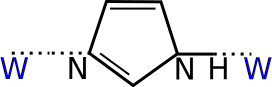
\includegraphics[width=0.4\linewidth]{Intro/Fig/SolvatedRotamer}  
      \caption{Water molecules placement around aromatic nitrogen in histidine residue functional group.}
      \label{Fig:SolvatedRotamer}
    \end{centering}
\end{figure}
The water molecules placement around the protein was derived by the authors from X-Ray crystallographic structures solved at high resolution. To avoid combinatoric explosion of
the number of solvated rotamers they restricted the placement of water molecules to the non-adjacent sites in a protein.

The other approach was implemented in the algorithm WATGEN \cite{bui2007watgen}. First, the hydrogens are added to the interacting proteins. These hydrogens, that interact with 
the atoms of a protein are called donors. Afterwards, all possible positions of water molecules are generated and those which have clashes with the atoms of the two proteins are
discarded. Then, the water sites are selected based on the number of interactions they are involved into. Additionally, two water sites closer than 0.5\AA~ are considered equal.
Finally, geometry of the water hydrogens is optimized to maximize the number of interactions.



\subsubsection{Multimeric docking}
Methods and algorithms described previously are applicable mainly to the problem of doking dimeric protein-protein complexes. However, 
many proteins in a cell form multimeric assemblies that play crucial role in recycling of the proteins in a cell, folding of the proteins, translation, transcription and many other 
vital cellular processes. There are two major ways in deciphering the structure of a multimeric complex starting from its subunits. The first type of programs
do not rely on any other information except for the possible symmetry of a complex and the structures of its subunits. The second one uses low-resolution
electron density maps, obtained from cryo-EM or small angle neutron scattering experiments.

The first class of methods deals with complexes of two general types: symmetric and nonsymmetrical.
The number of packages that can do symmetry-based multimeric docking is quite small: SymmDock \cite{schneidman2005geometry}, 
can build complexes with cyclic symmetry; Rosetta program protocol, that uses Monte-Carlo approach and can take into account cyclic, dihedral, helical and
icosahedral symmetries \cite{andre2007prediction}; M-ZDOCK \cite{pierce2005m} reduces rotational search space assuming cyclic symmetry and relies on FFT-based docking approach, \emph{etc}.

A few programs can dock proteins into nonsymmetrical complexes: CombDock \cite{inbar2005prediction} uses combinatorial approach, generating all pairwise 
pairs and finding among them tripples with the optimal score; Kim and Hummer algorithm \cite{kim2008coarse}, which uses Monte-Carlo approach and coarse-graining the protein models, 
HADDOCK \cite{dominguez2003haddock}; ATTRACT \cite{zacharias2003protein}; Multi-LZerD \cite{esquivel2012multi} and DockTrina \cite{popov2014docktrina}.

However, despite the variety of methods, they still perform poorly even on a simple benchmark \cite{popov2014docktrina}. The most reliable and widely-used technique 
to obtain atomic structure of a multimeric assembly is the docking of subunits into a low-resolution electron density map, usually obtained from cryo-EM experiments.

\paragraph{Docking proteins into low-resolution electron density map}
For this task, a number of software packages have been developed. 
Most notable of them are Situs \cite{Wriggers2010,Chacon2002}, NORMA \cite{Suhre2006},
EMFit \cite{Rossmann2001}, UROX \cite{Siebert2009}, etc. Despite the
differences in the implementation, all algorithms maximize
some score that shows the goodness of the fitting using a certain
optimization algorithm. An excellent review on different types of
the scoring functions used for cryo-EM density fitting is given by
Vasishtan and Topf \cite{Vasishtan2011}. According to them, one of
the most popular scoring functions is the cross-correlation function
(CCF) between the EDM and the density of the fitted protein. 

Given a protein structure that is described by its electron density $f(\mathbf{r})$,
and an EDM obtained from e.g. a cryo-EM experiment described by the function
$g(\mathbf{r})$, we can minimize the square root discrepancy between
them. Precisely, this discrepancy is given by
\begin{equation}
S=\int d\mathbf{r}\,\left(\hat T \hat R f(\mathbf{r})-g(\mathbf{r})\right)^{2},
\end{equation}
where $\hat T$ and $\hat R$ are the operators of the translation and the rotation
respectively, applied to the density $f(\mathbf{r})$. We can rewrite
the scoring function $S$ as 
\begin{equation}
S=\int d\mathbf{r}\,\left(\hat T \hat R f (\mathbf{r})\right)^{2}+\int d\mathbf{r}\, g^{2}(\mathbf{r})-2\int d\mathbf{r}\, \hat T \hat R f(\mathbf{r})g(\mathbf{r})
\end{equation}
Therefore, the minimization of the score $S$ is equivalent to the maximization
of the CCF: 
\begin{equation}
\textrm {CCF}=\int d\mathbf{r}\, \hat T \hat R f(\mathbf{r})g(\mathbf{r})
\end{equation}
with respect to the parameters of the operators $\hat T$ and $\hat R$. This
scoring function has been used in the majority of the algorithms and software
packages that perform the fitting into the EDM \cite{Wriggers2010,Siebert2009,Suhre2006}.

Another widely used scoring function is the Laplacian-filtered cross-correlation
function (LCCF). It originated from the observation that a human
performing a manual fitting a structure into an EDM tends to match
the isosurfaces of the densities rather than the densities themselves,
\begin{equation}
\textrm {LCCF}=\int d\mathbf{r}\,\left(\triangle \hat T \hat R f(\mathbf{r})\right)\left(\triangle g(\mathbf{r})\right)
\end{equation}
This scoring function works better than CCF for low resolution maps ($\sim 10-30$~\AA) \cite{Wriggers2010} and was used for the first time in the CoAn/CoFi
algorithm \cite{Volkmann1999}. Other scoring functions
that e.g. penalise symmetry-induced protein-protein contacts, or make use of protein-protein docking potentials, etc., have also been developed \cite{Vasishtan2011}.

  
  \newpage
  
  \section{Aim of work}
  This work deals with the protein-protein docking problem. The aim of the work was to propose and validate new algorithms in the area of 6D exhaustive
search and in the field of ranking the docking predictions. Particularly, the goal was to invent and test new ways to solve general global rigid-body search approaches that
could be more effective than the state-of-art in the field. In order to convincingly demonstrate their applicability, they have to be applied 
to one of the challenging problems, like fitting of cryo-EM electron density maps or rigid-body protein-protein docking and compared to the 
existing programs in the field.
The scoring method has to be applicable to a wide range of problems: from drug-like molecules docking to crystallographic water prediction.
It has to be free of methodological difficulties as in the case of statistical potentials, where the debates about the validity of the reference state 
computations are still going. This algorithm should be derived from the basic logical statements and have acceptable convergence properties.
   
\newpage
\chapter{Hermite fitting}

  \section{Introduction}
  As was already mentioned in the introduction, an important class of algorithms in computer science and structural biology deals with the exhaustive search in the 
six-dimensional space of translations and rotations of a rigid body. 

Modern exhaustive search algorithms either implement the fast 3D translational
search using the fast Fourier transform (FFT) \cite{Chacon2002,Katchalski-Katzir1992,Gabb1997,Wriggers2010,Siebert2009}
or the fast 3D rotational search by means of the spherical harmonics decomposition
and the FFT \cite{Kovacs2002} or even the fast 5D rotational search \cite{Kovacs2003,ritchie2008accelerating}.
Exhaustive search is also widely used as a preliminary step preceding the
local search or flexible refinement procedures. Thus, the quality
and the speed of the exhaustive search algorithms have a great impact on
the solution of the vast variety of problems. Therefore, we believe that new directions
of research on this topic are very important and highly valuable. 

In this section, we present the new HermiteFit algorithm that uses the orthogonal Hermite functions to perform exhaustive search in the 
six-dimensional space of rigid-body motions.
We apply this method to the problem of fitting of a high resolution X-ray structure of a protein subunit into the 
cryo-electron microscopy (cryo-EM) density map of a protein complex.
As a part of the new method, we developed an algorithm for the rotation of the decomposition in the Hermite basis and another algorithm for the conversion of
the Hermite expansion coefficients into the Fourier basis.
We demonstrate the ability of our algorithm to compete with the well--established approaches by using two examples of different difficulty, 
the PniB conotoxin peptide and the GroEL complex. 
%
The first example illustrates encoding principles and demonstrates the influence of the encoding quality on the goodness of  fit. 
%
The second example is the gold standard of all electron density map fitting 
algorithms. 
%
Our approach allows to analytically assess the quality of encoding of the Hermite basis using an estimation of the crystallographic R-factor. 
We then compare this estimation with the one computed numerically for the PniB conotoxin density map.
%
Finally, we compare the speed and the fitting accuracy of our algorithm with the two popular programs, the ADP\underline{\hspace*{0.2cm}}EM fitting method and the {\em colores} program from the 
Situs package and demonstrate that HermiteFit spends less running time per one search point compared to the two other methods while attaining a similar accuracy.

The HermitFit algorithm can be straightforwardly applied to a broad class of problems in different fields of research.
For example, one of the bottlenecks of the algorithms for molecular replacement in crystallography is the
computation of the Fourier coefficients (structure factors) of a molecule \cite{navaza1995fast}. 
This operation is to be precise and fast. However, the exact analytical evaluation 
of the structure factors is too costly \cite{sayre1951calculation} when recomputing them for each rotation of the molecule. 
Therefore, currently one uses the Sayre--Ten Eyck approach to compute the Fourier 
coefficients \cite{ten1977efficient}. Unfortunately, one has to be very careful tuning the parameters of the electron density model and
the grid cell size to obtain the desired precision \cite{navaza2002computation,afonine2003fast}.
Unlike the Sayre--Ten Eyck, our algorithm offers the analytical expression for the structure factors of the Hermite decomposition of a molecule.
%
Finally, our approach  allows to analytically estimate the quality of encoding using, e.g., crystallographic R-factors.

  \newpage
  
  \section{Methods}
  \subsection{Summary of the standard fitting algorithm}

The standard FFT-based 3D fitting algorithm operates according to
the workflow shown in Figure \ref{fig:CartesianFFT} \cite{Katchalski-Katzir1992,Gabb1997,Chacon2002}. The input of
this algorithm is a protein atomic structure determined experimentally
by, e.g., X-ray crystallography or nuclear magnetic resonance (NMR)
experiments. Another input is an experimental EDM
determined by means of, e.g., cryo-EM.
First, the algorithm decomposes
the experimental EDM into the Fourier basis using the fast Fourier
transform algorithm. Then, it rotates the protein
structure to a certain orientation $\mathbf{r}$ and decomposes the electron density of the
rotated structure into the Fourier basis. 

\begin{figure}[ht!]
\label{fig:CartesianFFT}
\caption[Flowchart of the standard fitting algorithm]{Flowchart of the standard fitting algorithm based on the Fourier correlations.
Green blocks correspond to the operations in the Fourier space.}
\includegraphics[width=1\textwidth]{Hermite/Fig/figure1}
\end{figure}

%
The electron density is typically computed as a sum of Gaussians centred on non-hydrogen atoms of the protein. 
%
Afterwards, the algorithm exhaustively
explores translational degrees of freedom of the rotated protein with
respect to the EDM. For every translation $\mathbf{t}$,
it determines the corresponding score, which is usually given by the
correlation between the two densities. This procedure is equivalent
to computing the convolution of two functions, 
\begin{equation}
\textrm{CCF}(\mathbf{r}, \mathbf{t})=\int d\mathbf{x}\, f(\mathbf{r},\mathbf{x}-\mathbf{t})g(\mathbf{x}),\label{eq:convolution}
\end{equation}
where $f(\mathbf{r},\mathbf{x-t})$ is the density of the protein rotated by $\mathbf{r}$ and translated by $\mathbf{t}$,
and $g(\mathbf{x})$ is the experimental electron density map. 
To speed up this step, the algorithm
computes the values of the Fourier transform of the CCF
for all translational degrees of freedom at once, using the convolution
theorem. Finally, the algorithm computes the inverse Fourier transform
(IFT) of the convolution, generates a new rotation of the protein
structure, and returns to the second step. This procedure is repeated
until all rotational degrees of freedom of the protein with respect
to the EDM are explored (see Fig. \ref{fig:CartesianFFT}). The solution
of the fitting problem is then given by $(\mathbf{r}_{max},\mathbf{t}_{max})=\mbox{argmax}_{\mathbf{r}, \mathbf{t}}\left\{ \textrm{CCF}(\mathbf{r}, \mathbf{t})\right\} $.


The bottleneck of the standard algorithm is 
the re-projection of the protein electron density into the Fourier space after each rotation.
%
%\blue{[Probably, we can stress this part more, as Lunin suggested]}
To overcome it, we propose to
encode the electron density of the protein structure in the orthogonal
Hermite basis, prior to performing the rotational search. This
allows to speed up the projection of the protein density into the
Fourier space. 
Since only the members of the Fourier family of linear transforms
can replace $O(N^2)$ operations of a convolution in a time domain by $O(N)$ operations in a frequency domain \cite{stone:1998}, we still need to
perform the convolution in the Fourier space.
%
Figure \ref{fig:FourierFitting} shows the workflow of the proposed algorithm.
Computational complexity of this algorithm is listed in Table \ref{table:FourierFitComp}.

\begin{figure}[H]
\label{fig:FourierFitting}
\includegraphics[width=1\textwidth]{Hermite/Fig/figure2}
\caption[Flowchart of HermiteFit]{Flowchart of HermiteFit, the new fitting algorithm based on the Hermite expansions.
Green blocks correspond to the operations in the Fourier space. Blue
blocks correspond to the operations in the Hermite space.}
\end{figure}

\begin{table}
\resizebox{\textwidth}{!}{
\begin{tabular}{|c|c|c|}
\hline 
Operation & Complexity & Loop multiplier \tabularnewline
\hline 
\hline 
Decomposition of the step function & 
$O(M^{3}\mbox{log}M^{3})$ & \multirow{4}{*}{1} \tabularnewline
\cline{1-2} 
Decomposition of the Gaussian & $O(N_{atoms}N^{3})$ & \tabularnewline 
\cline{1-2} 
Construction of the rotation matrix & $O(N_{rot}N^{4})$ & \tabularnewline
\hline  
Rotation & $O(N^{4})$ & \multirow{4}{*}{$N_{rot}$}\tabularnewline
\cline{1-2} 
Evaluation of the Hermite series & $O(M^{3}\cdot N+M^{2}\cdot N^{2}+M\cdot N^{3})$ & \tabularnewline
\cline{1-2} 
Multiplication & $O(M^{3})$ & \tabularnewline 
\cline{1-2} 
Inverse Fourier Transform & $O(M^{3}\mbox{log}M^{3})$ & \tabularnewline
\hline 
\end{tabular}
}
\medskip
\caption[Complexity of the Hermite fitting algorithm]{ Complexity of the Hermite fitting algorithm. Here, $M$ denotes
the order of the Fourier decomposition; 
$N$ is the order
of the Hermite decomposition; $N_{atoms}$ is the number of atoms in the
protein; $N_{rot}$ -- the number of rotations to be sampled.}
\label{table:FourierFitComp}
\end{table}

\subsection{Hermite functions}


Orthogonal Hermite function of order $n$ is defined as:
%
\begin{equation}
\psi_{n}(x;\lambda)=\frac{\sqrt{\lambda}}{\sqrt{2^{n}n!\sqrt{\pi}}}\exp(-\frac{\lambda^{2}x^{2}}{2})H_{n}(\lambda x),\label{eq:hermiteFunction}
\end{equation}
where $H_{n}(x)$ is the Hermite polynomial and $\lambda$ is the
scaling parameter. 
In Fig. \ref{fig:HermitePic} we show several orthogonal Hermite functions of
different orders with different parameters $\lambda$.
These functions form an orthonormal basis set in $L^2 \left( \mathbb{R} \right)$. A 1D function
$f(x)$ decomposed into the set of 1D Hermite functions up to an
order $N$ reads 
%
\begin{equation}
f(x)=\sum_{i=0}^{N}\hat{f}_{i}\psi_{i}(x;\lambda)\label{eq:decomposition}
\end{equation}
Here, $\hat{f}_{i}$ are the decomposition coefficients, which can
be determined from the orthogonality of the basis functions $\psi_{i}(x;\lambda)$.
Decomposition in Eq. \ref{eq:decomposition} is called the \emph{band-limited
decomposition} with $\psi_{i}(x;\lambda)$ basis functions. To decompose
the EDM and the protein structures, we employ the 3D Hermite functions:
%
\begin{equation}
\psi_{n,l,m}(x,y,z;\lambda)=\psi_{n}(x;\lambda)\psi_{l}(y;\lambda)\psi_{m}(z;\lambda),
\end{equation}
which form an orthonormal basis set in $L^2 \left( \mathbb{R}^3 \right)$. A function $f(x,y,z)$
represented as a band-limited expansion in this basis reads
%
\begin{equation}
f(x,y,z)=\sum_{i=0}^{N}\sum_{j=0}^{N-i}\sum_{k=0}^{N-i-j}\hat{f}_{i,j,k}\psi_{i,j,k}(x,y,z;\lambda)\label{eq:HermiteExpansion3D}
\end{equation}


\begin{figure}[H]
 \label{fig:HermitePic}
\begin{centering}
\includegraphics[width=1\textwidth]{Hermite/Fig/figure3}
\end{centering}
\caption[Hermite functions examples]{Left: 1D Hermite functions of order six for three different scaling
parameters $\lambda$. Right: 1D Hermite functions of two different
orders for the scaling parameter $\lambda=1$.}
\end{figure}

Figure \ref{fig:HermiteSin} shows that Hermite functions are very similar to the cosine functions near the coordinate axis origin. 

\begin{figure}[H]
 \label{fig:HermiteSin}
\begin{centering}
\includegraphics[width=1\textwidth]{Hermite/Fig/H50}
\end{centering}
\caption[Hermite functions and sine function]{Hermite function of the order 50 (solid line) and cosine function with the frequency equal to 50 (dashed line).}
\end{figure}

\subsection{Decomposition of electron densities into the orthogonal Hermite basis}
One of the advantages of the orthogonal Hermite basis is that we can
derive the exact analytical expression for the decomposition coefficients
of a molecular structure. This allows to rapidly obtain the exact
decompositions without costly numerical integration over the 3D space.
In our algorithm, the electron density of the protein ($f(x)$ in Eq. \ref{eq:convolution}, upon which rotation and translation operators act) 
is expanded in the Hermite basis using the Gaussian model.
More precisely, we model the electron density of a single atom in the molecular
structure as a Gaussian centred at the atomic position $\mathbf{r}_{0}^{(i)}$
with the squared variance equal to $\alpha^{2}/2$. Then, the electron
density of the whole molecular structure is given by the following
sum:
%
\begin{equation}
M(\mathbf{r})=\sum_{i=1}^{N_{atoms}}e^{-|\mathbf{r}-\mathbf{r}_{0}^{(i)}|^{2}/\alpha^{2}},\label{eq:protein_density}
\end{equation}
where $\mathbf{r}_{0}^{(i)}$ is the position of the $i$-th atom,
$\alpha/\sqrt{2}$ is the variance of the Gaussian distribution, and
$\mathbf{r}=(x,\, y,\, z)\in \mathbb{R}^{3}$ is the sampling volume. 
Normally, each Gaussian should be weighted with a coefficient corresponding to electron distribution of a particular atom. However, we omit the weights in our approximation.
In the section \ref{Sec: Shifted Gaussian expansion}, we provide analytical expressions (Eqs. \ref{eq:From1DTo3DCoeffs} and \ref{eq:Gaussian1DDecCoefs})
for the decomposition coefficients of $M(\mathbf{r})$ in the 1D and
the 3D cases.

\subsection{Shifted Gaussian expansion}
\label{Sec: Shifted Gaussian expansion}

Here we provide the derivation of the expansion coefficients of a
shifted Gaussian of the following form:
%
\begin{equation}
g(\mathbf{r})=e^{-\frac{|\mathbf{r}-\mathbf{r}_{0}|^{2}}{\alpha^{2}}}
\end{equation}
into the orthogonal Hermite basis. The well known property of this
basis (as well as of any orthogonal basis) is the following:
%
\begin{eqnarray}
\mbox{if }f(x,y,z) & = & f^{(1)}(x)f^{(2)}(y)f^{(3)}(z)\nonumber \\
\mbox{and }f^{(k)}(t) & = & \sum_{i=0}^{N}\hat{f}_{i}^{(k)}\psi_{i}(t;\lambda)\nonumber \\
 & \mbox{then}\nonumber \\
\hat{f}_{i,j,k} & = & \hat{f}_{i}^{(1)}\hat{f}_{j}^{(2)}\hat{f}_{k}^{(3)}\label{eq:From1DTo3DCoeffs}
\end{eqnarray}
First, we derive the decomposition of a 1D Gaussian into the 1D orthogonal
Hermite basis. Then, using property (\ref{eq:From1DTo3DCoeffs})
we obtain the decomposition of a 3D Gaussian into the 3D orthogonal
Hermite basis.
%
More specifically, the 1D Gaussian function reads as:
%
\begin{equation}
g(x)=e^{-\frac{(x-\xi)^{2}}{\alpha^{2}}}
\end{equation}
Its decomposition coefficients are equal to:
%
\begin{eqnarray}
\hat{g}_{n}(\xi;\lambda,\alpha) = \int\, g(x)\psi_{n}(x;\lambda)\, dx =  \nonumber \\ 
\frac{n!\sqrt{\lambda}e^{-\frac{\xi^{2}}{\alpha^{2}}\left(1-\frac{1}{\alpha^{2}\beta^{2}}\right)}}{\sqrt{2^{n}n!\sqrt{\pi}}} \sum_{m=0}^{[\frac{n}{2}]}\frac{(-1)^{m}}{m!(n-2m)!}  \nonumber \\ 
\int e^{-\beta^{2}\left(x-\frac{\xi}{\alpha^{2}\beta^{2}}\right)^{2}} (2\lambda(x-\frac{\xi}{\alpha^{2}\beta^{2}})+\frac{2\lambda\xi}{\alpha^{2}\beta^{2}})^{n-2m}dx   
,\end{eqnarray}
where $\beta^{2}=\frac{\lambda^{2}}{2}+\frac{1}{\alpha^{2}}$. From now on we will, for brevity, write $\hat{g}_{n}$ instead of
$\hat{g}_{n}(\xi;\lambda,\alpha)$. Changing the variables
$t=x-\frac{\xi}{\alpha^{2}\beta^{2}}$ and denoting $a=\frac{\xi}{\alpha^{2}\beta^{2}}$,
we obtain: 
%
\begin{eqnarray}
\hat{g}_{n} = \frac{n!\sqrt{\lambda}e^{-\frac{\xi^{2}}{\alpha^{2}}\left(1-\frac{1}{\beta^{2}}\right)}}{\sqrt{2^{n}n!\sqrt{\pi}}} \sum_{m=0}^{[\frac{n}{2}]}\frac{(-1)^{m}\left(2\lambda\right)^{n-2m}}{m!(n-2m)!} \nonumber \\ 
\int e^{-\beta^{2}t^{2}}(t+a)^{n-2m}dx\label{eq:gausCoeff}
\end{eqnarray}
Next, we decompose the sum $(t+a)^{k}$ using Newton's formula:
%

\begin{equation}
(t+a)^{k}=\sum_{i=0}^{k}\left(\begin{array}{c}
k\\
i
\end{array} \right)t^{i}a^{k-i}
\end{equation}
%
Thus, the integral in Eq. \ref{eq:gausCoeff} will read:
%
\begin{eqnarray}
\int e^{-\beta^{2}t^{2}}(t+a)^{n-2m}dx =  \nonumber \\ \sum_{i=0,\, i-even}^{n-2m}\frac{(n-2m)!}{2^{i}\left(\frac{i}{2}\right)!(n-2m-i)!}\sqrt{\pi}\beta^{-1-i}a^{n-2m-i}
\end{eqnarray}
Substituting it to the formula for $\hat{g_{n}}$ and denoting $\sum_{i=0,\, i-\textrm{even
}}^{n-2m}=\sum_{l=0}^{[\frac{n-2m}{2}]}$  $(i=2l)$,
we obtain the following expression for the coefficients:
%
\begin{eqnarray}
\hat{g}_{n}(\xi;\lambda,\alpha)=e^{-\frac{\xi^{2}}{\alpha^2}\left(1-\frac{1}{\alpha^{2}\beta^{2}}\right)}\sqrt{\frac{n!\sqrt{\pi}\lambda}{2^{n}}}\sum_{m=0}^{[\frac{n}{2}]}\,\,\sum_{l=0}^{[\frac{n-2m}{2}]}  \nonumber \\
\frac{(-1)^{m}2^{n-2m-2l}\lambda^{n-2m}}{l!(n-2m-2l)!m!}\beta^{-2n+4m+2l-1}\left(\frac{\xi}{\alpha^{2}}\right)^{n-2m-2l}\label{eq:Gaussian1DDecCoefs}
\end{eqnarray}
Finally, using Eq. \ref{eq:From1DTo3DCoeffs} we obtain a decomposition
of the 3D Gaussian into the 3D Hermite basis. We should note that
in order to avoid the rounding error, one should begin the summation
with the Gaussians that are located father from the origin.

\subsection{Expansion of a function defined on a grid}
In many docking algorithms the parwise interaction of particles is approximated as the set of functions on the grid. Therefore in many important cases the protein description goes beyond 
the sum of gaussians as in Eq. \ref{eq:protein_density}. In this section we provide a way to directly obtain decomposition of a function $f(x,y,z)$ defined on a regular grid. We can represent this 
function as a sum:
$$ f(x,y,z) = \sum_{i,j,k} f(x_i,y_j,z_k) \eta_{ijk}(x,y,z)$$
where $\eta_{ijk}(x,y,z)$ is a step-function in the position of $ijk$-th grid cell. Fig \ref{pic: stepFunction} shows the function $\eta$ that begins at point $a$ and has the width $h$.
To derive the decomposition of the general step-function in 3D and with arbitrary shift $a$ we have to begin with the basic 1D step-function that is fixed in $a=0$ point.

\begin{figure}[H]
\label{pic: stepFunction}
\begin{center}
\includegraphics[width=0.5\textwidth]{Hermite/Fig/StepFunction.pdf}
\end{center}
\caption[Shifted 1D step-function $\eta$]{Shifted 1D step-function $\eta$.}
\end{figure}

The expression for function is the following:
\begin{equation}
\eta(x)	=	
\begin{cases}
1, & 0\leq x<h\\
0, & \mbox{otherwise}
\end{cases}
\end{equation}
 
The decomposition coefficients of the shifted $\eta$ read:

\begin{eqnarray}
\eta(x-a)=\sum_{i}^{N}\alpha_{i}\psi_{i}(x;\lambda)\\
\alpha_{i}=\int_{-\infty}^{+\infty}\eta(x-a)\psi_{i}(x;\lambda)~ dx = \int_{a}^{h+a}\psi_{i}(x;\lambda)~dx 
\end{eqnarray}

We can obtain the coefficients $\alpha_n$ by simple integration:
\begin{equation}
\alpha_{n}=\frac{1}{\sqrt{2^{n}n!\sqrt{\pi}\lambda}}\int_{\lambda a}^{\lambda(h+a)}\exp(-\frac{t^{2}}{2})H_{n}(t)~ dt 
\end{equation}

Using the well known result for the finite integral of the Hermite polynomials:
\begin{equation}
 \int z^{q-1}e^{-pz^{2}}H_{n}(z)dz=n!\sum_{k=0}^{\left[\frac{n}{2}\right]}\frac{(-1)^{k-1}2^{n-2k-1}z^{n-2k+q}\left(pz^{2}\right)^{k-\frac{n+q}{2}}\Gamma\left(\frac{n+q}{2}-k,\, pz^{2}\right)}{k!(n-2k)!}
\end{equation}
with parameters $q=1$ and $p=1/2$ we obtain:
\begin{eqnarray}
 \int e^{-\frac{z^{2}}{2}}H_{n}(z)dz =\\ n!\left(\mbox{Sgn}[z]\right)^{n+1}&\sum_{k=0}^{\left[\frac{n}{2}\right]}\frac{(-1)^{k-1}\Gamma\left(\frac{n+1}{2}-k,\,\frac{z^{2}}{2}\right)}{2^{3k-\frac{3n}{2}+\frac{1}{2}}k!(n-2k)!}+C
\end{eqnarray}

After deriving the missing coefficients $C_n$ we obtain the following expression for the coefficients $\alpha_n$:
\begin{eqnarray*}
 \alpha_{n}=\frac{2^{n}\sqrt{n!}}{\sqrt{2\sqrt{\pi}\lambda}}\sum_{k=0}^{\left[\frac{n}{2}\right]}\frac{(-1)^{k-1}}{\left(2\sqrt{2}\right)^{2k}k!(n-2k)!}\\
 \left[\left(\mbox{Sgn}[h+a]\right)^{n+a}\Gamma\left(\frac{n+1}{2}-k,\,\frac{\left(\lambda h+\lambda a\right)^{2}}{2}\right)-\left(\mbox{Sgn}[a]\right)^{n+a}\Gamma\left(\frac{n+1}{2}-k,\,\frac{\left(\lambda a\right)^{2}}{2}\right)-\right.\\
 \left.\left(\left(\mbox{Sgn}[h+a]\right)^{n+1}-\left(\mbox{Sgn}[a]\right)^{n+1}\right)\Gamma\left(\frac{n+1}{2}-k,\,0\right)\right]
\end{eqnarray*}
Next, we are moving to the 3D case:
\begin{eqnarray*}
 \eta(x,y,z)&=&
 \begin{cases}
1, & 0\leq x<h_{x}\bigwedge0\leq y<h_{y}\bigwedge0\leq z<h_{z}\\
0, & \mbox{otherwise}
\end{cases} \\
\eta(x,y,z)&=&\eta(x;\, h_{x})\eta(y;\, h_{y})\eta(z;\, h_{z})\\
\eta(x-a_{x},\, y-a_{y},\, z-a_{z};h_{x},h_{y},h_{z})&=&\sum_{k}^{N}\sum_{j}^{N}\sum_{i}^{N}\alpha_{i}\alpha_{j}\alpha_{k}\psi_{i}(x;\lambda)\psi_{i}(y;\lambda)\psi_{k}(z;\lambda)
\end{eqnarray*}

As we see we have to multiply the coefficients of individual 1D-function with the shifts corresponding to the grid cell position along individual axes. We begin summation staring from the cells
that farther from the frame origin because rounding error substantially influences the final result.

\subsection{Laplacian filter in the Hermite basis}
For mid- to low- resolution maps the Laplacian-filtered cross-correlation function gives a better match compared to the CCF \cite{Wriggers2010}.
In the Hermite basis, the Laplacian filter has a particularly simple form.
Using the well-known recurrence relation for the derivatives of
the Hermite functions, we can easily derive the following relation for the second derivative of a 1D basis function:
\begin{equation}
 \frac{d^2}{d x^2}\psi_{n}(x; \lambda ) = \frac{\lambda^2}{2}\left( \sqrt{n(n-1)} \psi_{n-2}(x; \lambda ) + (2n+1)\psi_{n}(x; \lambda ) + \sqrt{(n+1)(n+2)} \psi_{n+2}(x; \lambda ) \right)
\end {equation}
A similar relationship holds for the coefficients of the decomposition: 
\begin{equation}
  \hat{h}''_{n} = \frac{\lambda^2}{2}\left(  \sqrt{n(n-1)} \hat{h}_{n-2} + (2n+1)\hat{h}_{n} + \sqrt{(n+2)(n+1)} \hat{h}_{n+2} \right)
  ,
\end {equation}
where $\hat{h}_{n}$ and $\hat{h''}_{n}$ are the n-th order decomposition coefficients of the original basis and its Laplacian representation,
respectively. For $n<0$ and $n>N$ we let $\hat{h}_{n} = 0$
and $\hat{h''}_{n} = 0$.
Due to the properties of the Laplace operator and the 3D Hermite decomposition, the contribution of the derivatives along each axis are additive. The derivation of the
formula for the 3D decomposition derivative is straightforward and we omit it for brevity.


\subsection{Rotation of the Hermite decomposition}

Recently, Park et al. \cite{Park2010} presented the method to perform
an in-plane rotation of a 2D orthogonal Hermite band-limited decomposition.
Here, we extend their method for the 3D case. Let us first consider
the decomposition of a 2D function into a 2D orthogonal Hermite function
basis:
%
\begin{equation}
f(x,y)=\sum_{n=0}^{N}\sum_{m=0}^{N-m}\hat{f}_{n,m}\psi_{n}(x;\lambda)\psi_{m}(y;\lambda)
\end{equation}
The decomposition of a function $f^{\theta}(x,y)$ rotated clock-wise by an angle
$\theta$ reads
%
\begin{equation}
f^{\theta}(x,y)=\sum_{m=0}^{N}\sum_{k=0}^{m}(\sum_{n=0}^{m}\hat{f}_{n,m-n}S_{k,n}^{m})\psi_{k}(x;\lambda)\psi_{m-k}(y;\lambda),\label{eq:2Drotation}
\end{equation}
where coefficients $S_{k,n}^{m}$ are computed using the following
recurrent formulas \cite{Park2010}:
%
\begin{eqnarray}
%\begin{split}
S_{q,n}^{m+1} &=&  \sqrt{\frac{n}{m-q+1}}\sin(\theta)S_{q,n-1}^{m}+  \sqrt{\frac{m-n+1}{m-q+1}}\cos(\theta)S_{q,n}^{m}\nonumber \\
S_{q,0}^{m+1}  &=&  \sqrt{\frac{m+1}{m-q+1}}\cos(\theta)S_{q,0}^{m}\nonumber \\
S_{m+1,n}^{m+1}  &=&  \sqrt{\frac{n}{m+1}}\cos(\theta)S_{m,n-1}^{m}-  \sqrt{\frac{m-n+1}{m+1}}\sin(\theta)S_{m,n}^{m}\nonumber \\
S_{m+1,0}^{m+1}  &=&  -\sin(\theta)S_{m,0}^{m}
%\end{split}
\end{eqnarray}
%
The key idea that allows to generalize these formulas to a 3D decomposition
is that we can factorize a rotation in 3D space into 3 independent
in-plane rotations around three different axes, and then rotate each
2D decomposition using Eq. \ref{eq:2Drotation}. Let us consider the
following 3D decomposition:
%
\begin{equation}
f(x,y,z)=\sum_{n=0}^{N}\psi_{n}(x;\lambda)\sum_{m=0}^{N-n}\sum_{l=0}^{N-m-n}\hat{f}_{n,m,l}\psi_{m}(y;\lambda)\psi_{l}(z;\lambda)
\end{equation}
If we rotate this decomposition about $x$ axis, this rotation will
be equivalent to  $N$ rotations of different 2D decompositions
in the $yz$-plane:
%
\begin{equation}
f_{n}(y,z)=\sum_{m=0}^{N-n}\sum_{l=0}^{N-m-n}\hat{f}_{n,m,l}\psi_{m}(y;\lambda)\psi_{l}(z;\lambda)
\end{equation}
This observation means that in order to perform such rotation, we
need to recompute rank-3 tensor of coefficients $\hat{f}_{n,m,l}$ slice
by slice $N$ times using Eq. \ref{eq:2Drotation}. Figure \ref{pic: rotationInterpretation}
illustrates three subsequent rotations of  tensor
$\hat{f}_{n,m,l}$. Each rotation of the coefficients in one plane
corresponds to a multiplication of these coefficients with a rotation
matrix. Therefore, a 3D rotation defined with three Euler angles is equivalent
to three sequential rotations of coefficients in three planes.

\begin{figure}[ht!]
\label{pic: rotationInterpretation}
\includegraphics[width=1\textwidth]{Hermite/Fig/figure4.pdf}
\caption[Rotations of the Hermite expansion]{Sequential rotations of coefficients $\hat{f}_{n,m,l}$ about different
axes. The rotated layer  is shown with the solid cubes, other coefficients
are shown with the dashed cubes.To perform the complete 
rotation of the decomposition about one axis, we rotate each layer
of coefficients about the corresponding axis in the space of coefficients.}
\end{figure}

%\subsection{Rotational invariants}

%In the previous section we described how coefficients of the Hermite decomposition change upon rotation of the density. However all intrinsic physical properties of the 
protein should not change upon rotation and translation of the reference frame. Therefore a description of the density that is invariant under rotation and translation 
is of great interest.

The rotational invariants originally were employed in 3D object recognition by Hue et all. \ref{hu1962visual}. To construct them they used geometrical moments:
$$M_{ijk}=\int\int\, f(x_{1},x_{2},x_{3})x_{1}^{i}x_{2}^{j}x_{3}^{k}\, dx_{1}\, dx_{2}\, dx_{3}$$
where $f$ stands for the density described and the integration is done over all 3D space where $f$ is defined.

After this peoneering work, much effort had been put into constructing invariants of geometric moments upon rotation, 
translation, general affine transformations and even projection operators. So far, several methods are available to 
construct systems of geometrical invariants \ref{hickman2012geometric, diao2009linear}. They are 
sucessfully applied in 2D pattern recognistion and 3D object recognition \ref{flusser2009moments} and positioning of 3D objects \ref{taubin1991recognition}.

However in many cases these moments are not the best choise. Other types of moments been investigated such as Legendre moments \ref{hosny2010new}, 
Zernike moments \ref{venkatraman2009protein} and others\ref{mak2008extension}. The Hermite-Gaussian moments haven't been previously explored in 3D, but they showed to be very 
useful in 2D image reconstruction \ref{yang2011image,rahman2013low}. In this section we provide a method to build 3D Hermite invariants.

First, by analogy with geometric invariants let's introduce Gaussian-Hermite invariants:
$$m_{pqr}=\int\int\int f(x,y,z)\psi_{p}(x)\psi_{q}(y)\psi_{r}(z)\, dx\, dy\, dz$$

The derivation of Hermite-Gaussian moments invariants is based on the exsting geometric moments invariants. Let's denote operator of rotation in $R^{3}$ as $\mathbf{R}$:
$r'=\mathbf{R}r$.
Geometric rotational invariants are algebraic functions of geometric moments that do not change their values after application of $\mathbf{R}$ operator. 
An example of such a function is:
$$I_{1}=\mu_{200}+\mu_{020}+\mu_{002}$$
which written in terms of integrals sums up to:
$$I_{1}=\int\int\int f(x,y,z)(x^{2}+y^{2}+z^{2})\, dx\, dy\, dz$$
The value of $I_{1}$ is simply a mass of the function, that is invariant upon rotations.
Let's now look closer at the integral form of Gaussian-Hermite moments:
$$m_{pqr}\propto \int\int\int f(x,y,z)e^{-(x^{2}+y^{2}+z^{2})/2\sigma^{2}}H_{p}(\frac{x}{\sigma})H_{q}(\frac{y}{\sigma})H_{r}(\frac{z}{\sigma})\, dx\, dy\, dz$$
Where the coefficient of proportionality does not depend on $x,y,z$ and therefore can be ommitted. The factor in the exponent is also invariant with
respect to the rotations and dos not influence the rotational behaviour of Hermite polynomials. Further we ommit these two factors.

Hermite polynomials can be further expanded in terms of $\frac{x}{\sigma}$, $\frac{y}{\sigma}$ and $\frac{z}{\sigma}$ and therefore each Hermite moment 
can be rewritten as the sum of monomials. For example:
$$m_{000} \propto  \int f(x,y,z) \, dx\, dy\, dz$$
$$m_{111} \propto  \int f(x,y,z) \left( 1 + 2\frac{x}{\sigma} \right)\left( 1 + 2\frac{y}{\sigma}\right)\left( 1 + 2\frac{z}{\sigma}\right)\, dx\, dy\, dz$$
%$$m_{222} \propto  \int f(x,y,z) \left( -1 + 2\frac{x}{\sigma} +4\left(\frac{x}{\sigma}\right)^2 \right)\left( -1 + 2\frac{y}{\sigma} +4\left(\frac{y}{\sigma}\right)^2 \right)\left( -1 + 2\frac{z}{\sigma} +4\left(\frac{z}{\sigma}\right)^2 \right)\, dx\, dy\, dz$$
Easy to see that $m_{111}$ behaves similar to the following combination of geometric moments:
$$m_{111}\propto \mu_{000} + 2\left(\mu_{100}+\mu_{010}+\mu_{001}\right) + 4\left(\mu_{110}+\mu_{011}+\mu_{101}\right) + 8\mu_{111}$$
On the other hand suppose we know several geometric invariants $I^(k) = f^k (\mu_{000},\mu_{100},\ldots)$. We now can eliminate variables $\mu_{ijk}$ in each
geometric invariant and obtain the Gaussian-Hermite invariants.

Summing up, the algorithm for deriving Gauss-Hermite invariants from geometric ones is:
\begin{enumerate}
 \item Get $k$-th geometric invariant $I_{k}^{G}(\mu_{000},...,\mu_{PQR})$
 \item From equations $m_{lmn}=M_{lmn}(\mu_{000},\ldots,\mu_{lmn}),~~ l=0\ldots L,~~ m=0 \ldots M,~~ p=0\ldots P$
  derive expressions for $\mu_{lmn}=M_{lmn}(m_{000},\ldots,m_{lmn}),~~ l=0\ldots L,~~ m=0 \ldots M,~~ p=0\ldots P$,
  where $P,Q,R \leq K$
 \item Substitute $\mu_{lmn}$ in geometric invariant $I_{k}$ for $M_{lmn}$
\end{enumerate}

The second step of the algorithm is valid because from the definition of Hermite polynomials the powers in products of $xyz$ do not exceed the order of moment. 
And therefore we have system of $K$ equations dependent on $K$ variables.

 

\subsection{Transition from the Hermite to the Fourier basis}
\label{Sec: HermiteFourierTransition}
In order to perform a fast convolution as in Eq. \ref{eq:convolution}, we
convert the decomposition coefficients from the Hermite basis into
the Fourier basis. This allows to use the fast convolution algorithm
based on the Fourier convolution theorem,
which was first introduced in protein-protein docking studies \cite{Katchalski-Katzir1992,Gabb1997}
and then also applied in the EDM fitting \cite{Chacon2002,Wriggers2010,Siebert2009}. 
The key idea of this algorithm is to compute the Fourier transform
of the values of a scoring function on a grid, $\textrm{CCF}(\mathbf{r}, \mathbf{t})=\int f(\mathbf{r},\mathbf{x})g(\mathbf{r},\mathbf{x}-\mathbf{t})d\mathbf{x}$,
using the convolution theorem:
%
\begin{equation}
F\left[f*g\right]=\overline{F}[f]F[g],
\end{equation}
i.e. to multiply the complex conjugated coefficients of the Fourier transform of the protein electron density
with the coefficients of the Fourier transform of the EDM. Then, we obtain $\textrm{CCF}(\mathbf{r}, \mathbf{t})$
by taking the inverse Fourier transform of $F\left[f*g\right]$,
%
\begin{equation}
\textrm{CCF}(\mathbf{r}, \mathbf{t})=\textrm{IFT}\left(\overline{F}[f]F[g]\right)
\end{equation}
%
Now we explain how we convert the decomposition coefficients from
the Hermite basis into the Fourier basis. 
Consider the decomposition
of a function $f(\mathbf{r})$ in the 3D Hermite basis with the decomposition
coefficients $\hat{f}_{i,j,k}$ (Eq. \ref{eq:HermiteExpansion3D}).
%
Orthogonal Hermite functions are the eigenfunctions of the continuous Fourier transform:
\begin{equation}
\int \psi_{n}(x;\lambda) e^{-2\pi i \omega x}~dx = (-i)^n \psi_{n}(\omega;\frac{2\pi}{\lambda})
\equiv \tilde{\psi}_{n}(\omega;\lambda),
 \label{Eq:HermiteFourierImage}
\end{equation}
where $\omega$ is the frequency in the reciprocal space.
%
In order to compute  Fourier coefficients of $f(\mathbf{r})$ up to order $M$,
we first compute the Fourier transforms of the basis functions $\psi_{i}(x;\lambda)$,
$\psi_{j}(y;\lambda)$, and $\psi_{k}(z;\lambda)$ using Eq. \ref{Eq:HermiteFourierImage}.
After, we substitute these coefficients into Eq. \ref{eq:HermiteExpansion3D} and obtain
the following expression for $\tilde{f}_{l,m,n}$, the Fourier coefficients
of $f(\mathbf{r})$:
\begin{equation}
\tilde{f}_{l,m,n}=\frac{1}{L_x L_y L_z}\sum_{i=0}^{N}\sum_{j=0}^{N-i}\sum_{k=0}^{N-i-j}\hat{f}_{i,j,k}\tilde{\psi}_{i}(\frac{l}{L_x};\lambda)\tilde{\psi}_{j}(\frac{m}{L_y};\lambda)\tilde{\psi}_{k}(\frac{n}{L_z};\lambda)
\label{eq:HermiteFourierSum}
\end{equation}
%where $L_x\times L_y\times L_z = V_{box}$ is the box volume.}
These values can be computed in $O(M^{3}\cdot N+M^{2}\cdot N^{2}+M\cdot N^{3})$
steps (see section \ref{Sec: Fast summation}).

\subsection{Fast summation}
\label{Sec: Fast summation}
%
Here we explain the fast summation in Eq. \ref{eq:HermiteFourierSumApp}: 
%
\begin{equation}
\tilde{f}_{l,m,n}=\sum_{i=0}^{N}\sum_{j=0}^{N-j}\sum_{k=0}^{N-i-j}\hat{f}_{i,j,k}\tilde{\psi}_{i,l}\tilde{\psi}_{j,m}\tilde{\psi}_{k,n}\label{eq:HermiteFourierSumApp}
,
\end{equation}
with indexes $l,m,n\in[0,M]$. The summation in this formula can
be performed with less operations than a naive estimation $O(M^{3}N^{3})$
suggests. We perform the fast summation by splitting the equation into
three consecutive sums:
%
\begin{equation}
\widetilde{T_{i,j,n}^{1}}=\sum_{k=0}^{N-i-j}\hat{f}_{i,j,k}\tilde{\psi}_{k,n}
\end{equation}
%
\begin{equation}
\widetilde{T_{i,m,n}^{2}}=\sum_{j=0}^{N-i}\widetilde{T_{i,j,n}^{1}}\tilde{\psi}_{j,m}
\end{equation}
%
\begin{equation}
\tilde{f}_{l,m,n}=\sum_{i=0}^{N}\widetilde{T_{i,m,n}^{2}}\tilde{\psi}_{i,l}
\end{equation}
%
It is easy to see that the construction of $\widetilde{T_{i,j,n}^{1}}$
matrix takes $O(MN^{3})$ operations, the construction of $\widetilde{T_{i,m,n}^{2}}$
matrix takes $O(M^{2}N^{2}$) operations, and the final summation
takes $O(M^{3}N$) operation. 
In the common use case ($N=15$, $M \gg N$) the last sum takes much more time than the other two.
To optimize it, we used the Gauss method to multiply complex numbers and expressed the whole sum as
a generalized matrix product of three real-valued matrices.  To implement
these operations, we used the ATLAS library.


\subsection{Implementation details and running time}
We chose to demonstrate the potential of the Hermite basis by implementing the rigid-body fitting of an atomistic structure of a protein in an electron density map of low resolution.
The  HermiteFit algorithm was implemented using the C++ programming language and compiled using g++ with -O3 optimization.
The running times of the tested algorithms are measured on a single core of an Intel$\textsuperscript{\textregistered}$ Xeon$\textsuperscript{\textregistered}$ CPU X5650 @ 2.67GHz 
processor with 24 GB of RAM on a Linux 64-bit operating system.

Our fitting method typically samples some $10^{10}$ rigid-body configurations. Therefore, it is practical to group its fitting solutions into clusters. There are multiple ways 
to measure the similarity between rigid-body solutions. For example, the pair-wise root--mean--square deviation (RMSD) is a fast and well-accepted similarity measure. 
Thus, we clustered the fitting solutions using the rigid-body clustering algorithm implemented with the RigidRMSD library \cite{popov2014rapid} as follows. 
%
First, the fitting solution with the best score (yet unassigned to any cluster) is taken as the seed for the new cluster. Second, the pair-wise RMSDs between the seed
and all other predictions are measured and the predictions with the RMSD lower than a certain threshold are put into the cluster. Finally, these two steps are iterated 
until all fitting predictions are assigned to corresponding clusters.


  \newpage
  
  \section{Analysis}
  This section provides analytical and numerical analysis of the density encoding in the Hermite basis. More specifically, we provide the choice of optimal model parameters and assess the quality of encoding. 

\subsection{Choice of parameters of the method}
Orthogonal Hermite functions (\ref{eq:hermiteFunction}) decay exponentially
after a certain distance and thus can encode information only within
some interval. We can estimate this interval using the formula for
the last root of a Hermite polynomial, $\xi_{1,N} \approx \frac{\sqrt{1+2N}}{\lambda}$
\cite{Math1995}, which gives an approximation for the half-size
of the bounding box that we can successfully encode:
%
\begin{equation}
L_{box}/2 \lesssim \frac{\sqrt{1+2N}}{\lambda}
\label{eq:encodingRegion}
\end{equation}
On the other hand, orthogonal Hermite functions are the eigenfunctions of the continuous Fourier transform (Eq. \ref{Eq:HermiteFourierImage}).
Therefore, Hermite decomposition of order $N$ can encode only a certain interval of frequencies.
Using the same approximation as in the case of the real-space interval, we obtain the following equation for the maximum encoding frequency:
\begin{equation}
\omega_{max}=\frac{\lambda}{2\pi}\sqrt{2N+1} \label{eq:OmegaMax}
\end{equation}
%
In case of the the Fourier series expansion on an interval $(0, L_{box})$, we can
use the same estimation for the maximum encoding index $M_{max}$ by setting $M_{max}=2L_{box} \omega_{max}$.
%
Resolution $R$  of an X-Ray electron density map is defined by the size of the reciprocal lattice as $R=1/(2\omega_{max})$, or, equivalently,  $R=L_{box} /M_{max}$.
Therefore, using resolution of the map $R$ and the order of the Fourier series expansion $M$, we can estimate the lower bound on the Hermite scaling parameter $\lambda$ required to encode all the reflexes of the electron density diffraction pattern to be
\begin{equation}
\lambda\gtrsim\frac{\pi}{\max(R,L_{box}/M)\sqrt{2N+1}} \label{eq:levelOfDetails}
\end{equation}
%
Here, we bounded the actual resolution by $L_{box}/M$, because this will be the limit allowed by the finite Fourier series of order $M$. 

The two inequalities (\ref{eq:encodingRegion}  and \ref{eq:levelOfDetails})
give approximate bounds on the scaling parameter $\lambda$,
provided that we know the size of the box $L_{box}$ containing a protein density and the resolution of the map $R$. 
Using these inequalities, we obtain the following relationship between parameters $\lambda$ and $N$:
%
\begin{equation}
\frac{\pi}{\sqrt{2N+1}\max(R,L_{box}/M)}\lesssim\lambda\lesssim2\frac{\sqrt{1+2N}}{L_{box}}\label{eq:relationLabmdaN}
,
\end{equation}
which is valid for sufficiently large values of $N$. 
%\blue{[The left bound defines the encoding square of the T-matrix. The right bound defines the amount of noise in the encoding square.]}
%
Nonetheless, we can use the following empirical estimation for the optimal value of $\lambda$ at any $N$:
\begin{equation}
\lambda_{opt} \approx \frac{\pi}{2\max(R,L_{box}/M)\sqrt{2N+1}}+\frac{\sqrt{1+2N}}{L_{box}}\label{eq:LambdaEstimate}
\end{equation}
%
Using dimensionless relative parameters $\lambda L_{box}$ and $L_{box}/R$ we may rewrite the previous expression as
\begin{equation}
\lambda L_{box} \approx \frac{\pi \min(L_{box}/R,M)}{2\sqrt{2N+1}}+\sqrt{1+2N}\label{RelativeEstimate}
\end{equation}
%
If at a given expansion order N there is no such parameter $\lambda$ that satisfies inequality  (\ref{eq:relationLabmdaN}), then 
the protein representation might involve information loss. Therefore, we can estimate the minimum
order $N_{min}$ of the Hermite expansion that allows this inequality to have solutions to be
\begin{equation}
N_{min} \approx \frac{\pi }{4} \min \left(\frac{L_{box}}{R} , M\right)
\label{eq:Nmin}
\end{equation}
Validity of the provided estimates and the graphical representation of the real--space and the reciprocal--space bounds on parameter $\lambda$
will be demonstrated in the following sections.


The maximum order of the Fourier expansion $M_{max}$ can be estimated from the resolution and the size of the density map as  $R=L_{box} /M_{max}$.
However, when finding the global maximum of the cross-correlation function, we need to sample the space of possible translations of a protein with respect to the EDM with a step several times finer than the EDM resolution $R$.
%
In protein crystallography, it is the common practice to set the 
sampling step size to $R/3$ \cite{afonine2003fast}. 
In principle, we can use the same reasoning in choosing the optimal number of rotations $N_{rot}$. 
%For example, 
When using spherical harmonics, the angular search step usually equals to the resolution of the basis, $2\pi/N$ \cite{garzon2007adp_em}.
In case of the Hermite basis, we propose to use the same criterion.



\subsection{The transfer matrix}
Below we describe an analytical model of encoding by the Hermite basis for the one-dimensional case.
Suppose we have a function  $f(x)$ that describes an electron density of a non-periodic object. 
Without loss of generality, we assume that this function is defined on a 1D interval of $(-L_{box}/2;+L_{box}/2)$.
This function has the following decomposition into Fourier series:
\begin{equation}
\tilde{f}^{exact}_{k} = \frac{1}{L_{box}}\int_{-L_{box}/2}^{+L_{box}/2} f(x)e^{-2\pi i k x/L_{box}}~dx
\end{equation}
We will refer to Fourier coefficients obtained using this expression as {\em exact}. 
%
The original function is then recovered by the inverse Fourier transform:
\begin{equation}
f(x) = \sum_{k=-\infty}^{+\infty} \tilde{f}^{exact}_{k}e^{2\pi i k x/L_{box}}
\end{equation}
%
On the other hand, our algorithm computes {\em approximate} Fourier coefficients using the Hermite to Fourier transform:
\begin{equation}
 \tilde{f}^{approx}_k=\frac{1}{L_{box}}\sum_{n=0}^{N}\hat{f}_{n}\tilde{\psi}_{n}(\frac{k}{L_{box}}; \lambda)
 \end{equation}
 %
Assuming that function $f(x)$ is zero outside of the bounding interval, Hermite coefficients $\hat{f}_{n}$ can be written as the finite integral:
%by assuming that the function is zero outside of the box:
\begin{equation}
\hat{f}_{n} = \int_{-L_{box}/2}^{+L_{box}/2} f(x) \psi_{n}(x; \lambda)~dx
\end{equation}
%
Now, we can express the {\em approximate} Fourier coefficients as a linear combination of the {\em exact} ones:
\begin{equation}
\tilde{f}^{approx}_{k} = \sum_{l=-\infty}^{+\infty} T_{k,l} \tilde{f}^{exact}_{l}, 
\label{Eq:fourierApproximation}
\end{equation}
where the  {\em transfer matrix} $T_{k,l}$ reads as:
\begin{equation}
T_{k,l} = \frac{1}{L_{box}}\sum_{n=0}^{N}  \tilde{\psi}_{n}(k; \lambda) \int_{-L_{box}/2}^{+L_{box}/2} \psi_{n}(x; \lambda) e^{2\pi i l x/L_{box}} dx~
\label{eq:Tmatrix}
\end{equation}
%
The transfer matrix acts as a linear filter in the reciprocal space and demonstrates how the input function is distorted by the finite size $N$ of the Hermite basis. 
We should note that, generally, its values are complex numbers.
%
This matrix can also be seen as a product of two matrices,
\begin{equation}
\bf T = \bf F^{(1)} \bf F^{(2)},
\label{eq:TmatrixProduct}
\end{equation}
where the first matrix is a scaled Fourier transform of the basis functions,
\begin{equation}
 F^{(1)}_{kn} =  \tilde{\psi}_{n}(k; \lambda) / \sqrt{L_{box}}
\label{eq:F1matrix}
\end{equation}
and the second matrix is  a scaled Fourier series of the basis functions,
\begin{equation}
F^{(2)}_{nl} = \int_{-L_{box}/2}^{+L_{box}/2} \psi_{n}(x; \lambda) e^{2\pi i l x/L_{box}} dx / \sqrt{L_{box}}
\label{eq:F2matrix}
\end{equation}
%
Figure \ref{fig:HermiteFDec} shows the absolute values of matrices $ \bf F^{(1)} $ and $\bf F^{(2)}$ computed with $\lambda=0.55$ and $L_{box}=23$ \AA. 
%
The values of the  Fourier series  $\bf F^{(2)}$ were computed numerically using adaptive  quadrature.
%
The dashed blue line shows the maximum encoding frequency $\omega_{max}$, according to Eq. \ref{eq:OmegaMax}, and bounds the encoding region. 
The solid black line on the right plot demonstrates the maximum order of the Hermite expansion (Eq. \ref{eq:encodingRegion}), after which the 
Fourier series encode mainly the frequencies near $\omega_{max}$.  This is because on a finite interval $(-L_{box}/2 ,+L_{box}/2)$, 
high-order Hermite basis functions become orthogonal to low-order Fourier basis functions. 
%

\begin{figure}[H]
\label{fig:HermiteFDec}
\begin{centering}
\includegraphics[width=\textwidth]{Hermite/Fig/HermiteFTransformAndSeries.pdf}
\par\end{centering}
\caption[Matrices $\bf{F^{(1)}}$ and $\bf{F^{(2)}}$]{
Absolute values of two matrices $\bf{F^{(1)}}$ and $\bf{F^{(2)}}$ that give the transfer matrix as their product (Eq. \ref{eq:TmatrixProduct}). These matrices are computed with the scaling parameter $\lambda=0.55$ and the input box size of $L_{box}=23.0$ \AA, which mimics
the first fitting example shown below.
Left: $\bf{F^{(1)}}$, the scaled Fourier transform of a 1D Hermite function as given by Eq. \ref{eq:F1matrix}. 
Right: $\bf{F^{(2)}}$, the scaled Fourier series of a 1D Hermite function as given by Eq. \ref{eq:F2matrix}.
The dashed blue line highlights the maximum encoded frequency according to Eq. \ref{eq:OmegaMax}.
The solid black line on the right plot shows the maximum Hermite decomposition order  $N_{max}$, at which the two matrices are still identical (Eq. \ref{eq:encodingRegion}).
}
\end{figure}


Figure \ref{fig:TmatrixesVsLambda} shows several examples of the absolute values of the transfer matrix components for three different values of the Hermite scaling parameter $\lambda$ and three values of the Hermite decomposition order
$N$.
The size of the transfer matrix was limited to $60\times 60$ and the box size $L_{box}$ was set to 23 \AA. 
The ideal transfer matrix should be identity, which is the case only at $N\rightarrow\infty$, as we demonstrate below.
We see, however, that the transfer matrix at small values of $\lambda$ encodes only low-order reflexes. 
The index of the last encoded reflex can be estimated from Eq. \ref{eq:OmegaMax} as $k_{max}=\sqrt{2N+1}\lambda L_{box}/(2\pi)$.
With the increase in  order $N$ and  parameter $\lambda$, the number of encoded frequencies  rises. 
At the same time, 
increasing the scaling parameter $\lambda$ makes the quality of encoding of all the frequencies worse, as we see in the right column. 
Therefore, it is very important to tune the value of $\lambda$ according to the class of input functions, such that the quality of encoding becomes optimal.
Below we will assess encoding quality by means of the  crystallographic R-factor.

\begin{figure}[H]
\label{fig:TmatrixesVsLambda}
\begin{centering}
\includegraphics[width=\textwidth]{Hermite/Fig/TmatrixesPlot.png}
\par\end{centering}
\caption[Transfer $T$-matrices]{Nine examples of the absolute values of the transfer $T$-matrices for three different values of $\lambda$ and  three different values of the Hermite decomposition order $N$. 
The number of Fourier coefficients is $M=60$, and the input box size is $L_{box}=23.0$ \AA, which mimics
the first fitting example shown below.
Hermite decomposition orders are $N\in\{15, 20, 30\}$, parameter $\lambda$ takes the values of 0.3 \AA$^{-1}$, 0.55 \AA$^{-1}$, and 1.0 \AA$^{-1}$.
The first column corresponds to the relative $\lambda L_{box}$ value of 6.9, the middle column corresponds to the relative $\lambda L_{box}$ value of $12.65$, and the 
right column to the relative $\lambda L_{box}$ value of $23$.
Notably, at low values of $\lambda$ the transfer matrix encodes only small order reflexes. The index of the last reflex can be estimated  from Eq. \ref{eq:OmegaMax} as $k_{max}=\frac{\sqrt{2N+1}\lambda L_{box}}{2\pi}$.
Increasing the value of $\lambda$, the number of encoded frequencies rises. However, at the same time, the quality of encoding of low frequencies worsens, as can be seen from the values at the diagonal.
}
\end{figure}

\subsection{Asymptotic behaviour of the transfer matrix}
Here we demonstrate that the transfer matrix asymptotically  achieves the  Kronecker delta function at $N\rightarrow\infty$.
%[To gain deeper understanding of the T-matrix behaviour we show the assimptotics of this matrix for $N\rightarrow\infty$.] 
Recall the Mehler's formula \cite{Mehler1866ueber}:
\begin{equation}
\sum_{n=0}^N u^n \psi_n(x)\psi_n(y)=\frac{1}{\sqrt{\pi(1-u^2)}} \exp \left( -\frac{1-u}{1+u}\frac{(x+y)^2}{4} - \frac{1+u}{1-u}\frac{(x-y)^2}{4} \right)
\end{equation}
If we rewrite the transfer matrix in the following way:
\begin{equation}
T_{k,l} = \frac{1}{L_{box}} \int_{-L_{box}/2}^{+L_{box}/2}dx~ \sum_{n=0}^{N}(-i)^n \psi_{n}(\frac{k}{L_{box}}; \frac{2\pi}{\lambda}) e^{2\pi i l x/L_{box}}\psi_{n}(x; \lambda),
\end{equation}
and use the fact that
\begin{equation}
\psi_{n}(x; \lambda) \equiv \sqrt{\lambda}\psi_{n}(\lambda x),
\end{equation}
we see that we can use the Mehler's formula to compute the limit
\begin{equation}
\lim_{N\rightarrow\infty} \sum_{n=0}^{N} (-i)^n \psi_{n}(\frac{k}{L_{box}}; \frac{2\pi}{\lambda})\psi_{n}(\frac{l}{L_{box}}; \lambda)
\end{equation}
%
After a simple derivation, we obtain the final result:
\begin{equation}
\lim_{N\rightarrow\infty}T_{k,l} = \frac{1}{L_{box}} \int_{-L_{box}/2}^{+L_{box}/2} e^{2\pi i l x/L_{box}} e^{-2\pi i k x/L_{box}} dx,
\end{equation}
which is exactly the Kronecker delta function.


\subsection{Encoding quality}
There are several ways to evaluate the quality of a model encoding with the subsequent reconstruction. 
For example, in the optimal control theory \cite{boyd1991linear}, the quality of a linear filter is estimated using a certain norm of the transfer matrix.
However, in crystallography, the most used quality criterion is the crystallographic R-factor \cite{stout1968x}:
\begin{equation}
R = \frac{ \sum_{l}\left|\left|\tilde{F}_{l}^{exact} \right| - \left|\tilde{F}_{l}^{mod} \right| \right|}{\sum_{l}\left|\tilde{F}_{l}^{exact} \right|}
,\label{eq:Rfactor}
\end{equation}
where $F^{exact}$ and $F^{mod}$ are the exact Fourier coefficients of a molecule and the coefficients computed from the Hermite coefficients, respectively.
This quantity is a widely used measure of agreement between a crystallographic model and the corresponding experimental X-ray diffraction data. In the case of an ideal electron density
encoding, R-factor is equal to zero. In protein crystallography, models with R-factors less than 0.2 are regarded as good when working at a middle resolution.

%
Equations for the transfer matrix allow to estimate the R-factor values for certain classes of electron density distributions. 
As described above (Eq. \ref{eq:protein_density}), we use the Gaussian distribution to model the electron density of an atom. 
%
Exact Fourier coefficients of a molecule with $N_{atoms}$ atoms at positions $\mathbf{r}_{i}$ are then given as: 
\begin{equation}
{\tilde f}_{l,m,n}^{exact}({\bf s})= \alpha^3 \pi^\frac{3}{2} \sum_{i=1}^{N_{atoms}} e^{ - \alpha^2 \pi^2 {\bf s}_{lmn}^2  } e^ { -2 i \pi \mathbf{r}_{i} {\bf s}_{lmn} }
,\label{eq:ExactCoef}
\end{equation}
where $s_{l,m,n}$ is the wave vector,  ${\bf s}_{l,m,n}=\left( l/L_x,m/L_y,n/L_z \right)$, with $L_x$, $L_y$,  and $L_z$ the dimensions of the bounding box along the corresponding axes.
Similarly, one-dimensional exact Fourier coefficients of the Gaussian function are given as:
\begin{equation}
{\tilde f}_{l}^{exact} =\alpha \pi^\frac{1}{2} \sum_{i=1}^{N_{atoms}} e^{ - \alpha^2 l^2 / L_{box}^2 } e^ { -2 i \pi {r}_{i} l /  L_{box}}
\label{eq:ExactCoef1D}
\end{equation}
To see how the Hermite basis encodes Gaussian densities with various level of detail, we built models of electron density map with different parameters $\alpha$. The 
width of the Gaussian determines the resolution of the density map according to:
\begin{equation}
R=\frac{\pi\alpha}{2}
\label{eq: densityModelAlphaVsResolution}
\end{equation}
The derivation of this formula follows the one well known in crystallography, which describes the extinction of diffraction reflexes. For the sake of completeness of the thesis, we provide 
its derivation in the section \ref{Sec: ResolutionModel}.

To estimate R-factor for certain model parameters, we assume that the input electron density is given as a sum of Gaussians with variance of $\alpha/\sqrt{2}$ equispaced at a distance $\alpha$.
Figure \ref{fig:RfactorsVsNVsLambda} shows analytical R-factors in one dimension computed using Eqs. \ref{Eq:fourierApproximation} and \ref{eq:ExactCoef1D}
as a function of the Hermite decomposition order $N$ and the scaling parameter $\lambda$.
We bounded the input and output frequencies by $M=30$ Fourier coefficients. The size of the input interval $L_{box}$ is set to 23.0 \AA ~ to mimic
the alpha-conotoxin PnIB peptide (pdb code 1AKG) decomposition used in the fitting example below.

\begin{figure}[h]
\label{fig:RfactorsVsNVsLambda}
\includegraphics[width=\textwidth]{Hermite/Fig/RfactorsLamN.pdf}
\caption[Analytical R-factors]{
Analytical R-factors in one dimension as a function of Hermite decomposition order $N$ and scaling parameter $\lambda$ computed at three different resolutions.
The input signal is modelled as a sum of Gaussians (Eq. \ref{eq:protein_density}) with the variance of $\alpha/\sqrt{2}$ equispaced at a distance $\alpha$. The number of Fourier coefficients is $M=30$, and the input box size is $L_{box}=23.0$ \AA.  These values are chosen to mimic
the 1AKG peptide decomposition. The estimate on the optimal parameter $\lambda$ (Eq. \ref{eq:LambdaEstimate}) is plotted with the red dashed line. 
The real-space bound on the optimal parameter $\lambda$  (Eq. \ref{eq:encodingRegion}) is shown with the orange dashed line. The reciprocal-space bound on the optimal parameter $\lambda$  (Eq. \ref{eq:levelOfDetails}) is shown with the blue dashed line.
{\bf Left}: The Gaussian parameter $\alpha=0.2$ \AA, corresponding to the absolute input signal resolution of $R=0.31$ \AA~ and the relative resolution of  $R/L_{box}=0.014$. However, in this case, the actual absolute resolution is cut at $L_{box}/M=0.77$ \AA, which corresponds to the relative resolution of 0.033.
{\bf Middle}: The Gaussian parameter $\alpha=1.0$ \AA, corresponding to the absolute input signal resolution of $R=1.57$ \AA~ and the relative resolution of  $R/L_{box}=0.068$.
{\bf Right}: The Gaussian parameter $\alpha=5.0$ \AA, corresponding to the absolute input signal resolution of $R=7.85$ \AA~ and the relative resolution of  $R/L_{box}=0.34$.
}
\end{figure}

%
We should stress that due to the properties of the Hermite functions, 
the whole model is scale--invariant. More precisely, if we keep the product $\lambda L_{box}$ constant, then the relative shape of the Hermite basis functions would not change. Also, if we scale $L_{box}$ and $\alpha$ simultaneously, then the value of R-factor is unchanged. 
%
Therefore, it is useful to provide relative resolutions computed as  $R/L_{box}$.
%
Figure \ref{fig:RfactorsVsNVsLambda} (Left) shows R-factors for the Gaussian parameter $\alpha=0.2$ \AA, corresponding to the absolute input signal resolution of $R=0.31$ \AA~ and the relative resolution of  $R/L_{box}=0.014$. However, in this case, the actual absolute resolution is cut at $L_{box}/M=0.77$ \AA, which corresponds to the relative resolution of 0.033.
%
Figure \ref{fig:RfactorsVsNVsLambda}  (Middle) shows R-factors computed using the Gaussian parameter $\alpha=1.0$ \AA, corresponding to the absolute input signal resolution of $R=1.57$ \AA~ and the relative resolution of  $R/L_{box}=0.068$.
Figure \ref{fig:RfactorsVsNVsLambda} (Right) shows R-factors computed using the Gaussian parameter $\alpha=5.0$ \AA, corresponding to the absolute input signal resolution of $R=7.85$ \AA~ and the relative resolution of  $R/L_{box}=0.34$.
%
The estimate on the optimal parameter $\lambda$ (Eq. \ref{eq:LambdaEstimate}) is plotted with the red dashed line. 
The real-space bound on the optimal parameter $\lambda$  (Eq. \ref{eq:encodingRegion}) is shown with the orange dashed line. The reciprocal-space bound on the optimal parameter $\lambda$  (Eq. \ref{eq:levelOfDetails}) is shown with the blue dashed line.
We see that lowering the resolution of the input signal, R-factors decrease, as can be expected from general considerations. We can also see that the the lower (Eq. \ref{eq:encodingRegion}) and the upper (Eq. \ref{eq:levelOfDetails}) bounds on the optimal scaling parameter $\lambda$ follow the isolines of the R-factor map.
Therefore, their mean given by Eq. \ref{eq:encodingRegion} provides a reasonable estimation on the optimal value of $\lambda$.


Figure \ref{fig:RfactorsVsResolution} shows R-factors as a function of input signal resolution $R$ for three different Hermite decomposition orders $N$, 15, 20, and 30.
R-factors were estimated in the same way as in the previous case. 
More precisely, we assumed the same shape of input electron density and then used Eqs. \ref{Eq:fourierApproximation} and \ref{eq:ExactCoef1D} to compute the analytical R-factors. For these plots, we computed the optimal scaling parameter $\lambda$ using Eq. \ref{eq:encodingRegion}.
Parameter $L_{box}$ and the size of the transfer matrix $M$ were constant and equal to 23 \AA~ and $30$, correspondingly. As in the previous figure, these values are chosen to mimic
the alpha-conotoxin PnIB peptide decomposition used in the fitting example below.
%
The scale of the top horizontal axis gives the absolute resolution for $L_{box}=23$ \AA. The scale of the bottom horizontal axis gives  the relative resolution. In order to compute the absolute resolution, its values need to be multiplied by the chosen value of  $L_{box}$.
As expected, the values of R-factors diminish as the resolution becomes lower. This is because at low resolutions, low-frequency columns of the transfer matrix become more important.
In the limiting cases of zero and infinite resolutions, R-factor can be computed directly from the transfer matrix as a certain norm of $T-I$. For the infinite resolution limit, it is given as $L_1$ norm of the central column of matrix $T-I$. For the zero resolution limit, R-factor is given by the entry-wise $L_1$ norm of $T-I$, $R=\sum_{i,j}|T_{i,j}-\delta_{i,j}|$.
%
Figure 8 also shows an estimation of R-factors for the 3D case. It is based on the assumption that  the Hermite decomposition encoding in 
3D behaves similar to the 1D case, with the number of coefficients scaled as $N_{1D} = \sqrt[3]{N_{3D}}$.

\begin{figure}[H]
\label{fig:RfactorsVsResolution}
\begin{centering}
\includegraphics[width=0.5\textwidth]{Hermite/Fig/RfactorVsResolution_DiffAlphas.pdf}
\par\end{centering}
\caption[R-factors in one and three dimensions]{Analytical R-factors in one and three dimensions as a function of  relative resolution $R/L_{box}$. 
The absolute resolution at box size $L_{box}=23$ \AA~ is shown in the top horizontal axis.
Plots for three different Hermite expansions orders are shown, $N\in\{15,20,30\}$.
Parameters $L_{box}$ and $M$ were constant and equal to $23$ \AA~ and $30$, correspondingly. Scaling parameter $\lambda$ was estimated 
using  Eq. \ref{eq:LambdaEstimate}. }
\end{figure}

\subsection{Resolution model}
\label{Sec: ResolutionModel}
To illustrate the connection between parameter $\alpha$ in the model of electron density (Eq. \ref{eq:protein_density}) and the resolution of 
the X-ray diffraction pattern, we use the simplest model. More precisely, we model the electron density as the 
array of Gaussians in a perfect 1D lattice perpendicular to the incoming radiation beam. Parameter $\alpha$ then plays the role similar to the temperature B-factors.
X-ray diffraction intensity depends on the angle between the incoming beam and the direction to the detector $\theta$ as:
\begin{equation}
I \propto \left|\int dx~ f(x)\exp\left( 2\pi i x \frac{\sin\theta}{\lambda}\right)\right|^2
\end{equation}
where $\lambda$ is the wavelength of the incoming radiation. Using the model density (Eq. \ref{eq:protein_density}), we obtain:
\begin{equation}
I \propto \left|\alpha\sqrt{\pi}e^{-(\pi \frac{\sin\theta}{\lambda} \alpha)^{2}} \int dx~ \rho(x)\exp\left( 2\pi i x \frac{\sin\theta}{\lambda}\right)\right|^2
,
\end{equation}
where $\rho(x)$ is the sum of delta functions at the atomic positions. Therefore, the extinction of the diffraction peaks
is proportional to $\left|e^{-(\pi \frac{\sin\theta}{\lambda} \alpha)^{2}}\right|^2$, where we neglect the quadratic factor before the exponent. 
%
According to the definition used in crystallography, resolution is the inter-planar distance in the real space corresponding to the last observable peak in the reciprocal space. 
Unfortunately, the index of the last peak depends on the detector's noise and strongly depends on the characteristics of the measurement device. Therefore, to give qualitative estimation
on the dependence of resolution on the model parameter $\alpha$, we assume that the last observable peak is the one whose intensity decreases approximately by the factor $e^2$. 
The corresponding angle then reads:
\begin{equation}
\sin\theta_{max}=\frac{\lambda}{\pi\alpha}
\end{equation}
Therefore, the minimum inter-planar distance, or, the resolution is given by Bragg's law as:
\begin{equation}
R=\pi\alpha/2 \label{eq:RFactorAppendix}
\end{equation}

  
  \newpage
  
  \section{Results and Discussion}
  We tested and verified our algorithm using two examples of different difficulty.
The first example is a small polypeptide alpha-conotoxin
PnIB. We generated the EDM for this example from the coordinates of
the polypeptide. The second example is the fitting the GroEL domains
into the electron density map of the GroEL complex.

\subsection{Alpha-conotoxin PnIB}
First, we explored the relationship between encoding quality and the quality of the fitting. For this purpose, we chose the small 16--residue polypeptide alpha-conotoxin
PnIB. We downloaded the X-ray crystal structure of alpha-conotoxin PnIB (PDB code
1AKG) \cite{Guimond2009} from the PDB database \cite{Berman2000} and
simulated the electron density map (2mFo-DFc) using the Uppsala electron density server \cite{Kleywegt2004} with the resolution $R=1.1$ \AA.
We computed the protein density according to  Eq. \ref{eq:protein_density}
with the Gaussian width $\alpha=1.0$ \AA~ using
only the non-hydrogen atoms of the standard amino acids. We rotated the initial 1AKG structure by the arbitrarily chosen Euler angles equal to 
76, 234, and 56 degrees, respectively, and used it as the input for the fitting workflow.
We used $N_{rot}=500$ (corresponding to an angular step of 36\textdegree ) rotations represented with uniformly 
distributed Euler angles spanning the space of $2\pi\times\pi\times 2\pi$. 
The order of the Hermite expansion
was set to $N=15$, which is the minimum expansion order allowed at this resolution according to Eq. \ref{eq:Nmin}. 
The order of the Fourier expansion was twice the order of the Hermite expansion, $M=30$ for each dimension.

To see how the encoding quality influences the fitting algorithm, we studied the dependence of the decomposition on the scaling
parameter $\lambda$. We chose a range of $\lambda$ parameters between
0.05 and 2.0. For each $\lambda$, we computed the best fitting score along with the average fitting score. 
Fitting results are shown in Fig. \ref{fig:test1AKG}.
We see that by choosing $\lambda$ small,
we neglect the details of the protein structure (Fig. \ref{fig:test1AKG} A) and therefore, we can not discriminate between different orientations
of the protein (maximum score for $\lambda=0.05$ is very close to
the average score). When choosing $\lambda$ sufficiently large, we
obtain satisfactory discriminative power to find the near-native position
of the protein (Fig. \ref{fig:test1AKG} C,D). We also see that,
e.g., for $\lambda=0.5$, the difference between the maximum and the
average score is much larger than in the case of $\lambda=0.05$.
Also, when we take $\lambda$ too large, we can not encode the whole
protein (Fig. \ref{fig:test1AKG} E). 
%
The red dashed line on Fig. \ref{fig:test1AKG} shows R-factors computed with Eq. \ref{eq:Rfactor}.
We see that the choice of parameter $\lambda$ influences the R-factors and thus determines the quality of the fitting. 
Notably, the minimum of the R-factor curve corresponds to the maximum
of the fitting score.


Due to the strong influence of the scaling parameter $\lambda$ on the discrimination power of the algorithm,
we estimated its optimal value to gain the maximum separation between the score of the correct pose and the average score. 
%
Provided that the box that contains all the rotations of the peptide has the size $L_{box}=23$~\AA~and setting the resolution of the 
EDM $R=1.1$ {\AA}, Eq. \ref{eq:LambdaEstimate} gives an estimate on the optimal value of the scaling parameter $\lambda_{opt}\approx0.50$.
%
Fig. \ref{fig:test1AKG} shows
that this estimation corresponds to the best discrimination
between the near-native and all other structures, which can be deduced
from the maximum separation between the score of the prediction and
the average score. 
RMSD between the prediction and the solution at this value of $\lambda$ is $1.03$ \AA .
%
We should note that the RMSD can be  decreased by taking a finer angular search step.


\begin{figure}[h]
\label{fig:test1AKG}
\begin{centering}
\includegraphics[width=1\textwidth]{Hermite/Fig/ScoreDescriminationVsLambdaAndRFactor-rev.pdf}
\par\end{centering}
\caption[Results for the alpha-conotoxin PnIB]{Test of the fitting algorithm on artificially generated EDM for the alpha-conotoxin PnIB (PDB code 1AKG).
Here, we plotted the dependence of four parameters, the maximum score, the average score, the score of the near-native conformation and the crystallographic R-factor on the scaling
parameter $\lambda$. 
Isosurface of the Hermite decomposition at protein model density equal to $ (\rho_{max}+\rho_{min})/2 $ and several values of $\lambda$ are shown in sub-plots A ($\lambda=0.05$),
B ($\lambda=0.15$), C ($\lambda=0.3$), D ($\lambda=0.55$) and E ($\lambda=2.0$). }
\end{figure}

\subsection{GroEL complex}
Here, we demonstrate that our approach obtains essentially the same results as other programs, provided that the scoring function if the same (LCCF in this case).
For this purpose, we use a classical test for a fitting algorithm, the GroEL complex map. 
We downloaded the EDM of the GroEL complex from the Electron Microscopy Data Bank (EMDB), code EMD-2001 with 
resolution of 8.5~\AA.
Then, we downloaded the crystal structure of the GroEL subunits from the PDB database. We used the GroEL-GroES complex (PDB code 1AON), from which we extracted the chain A, 
centered it and arbitrary rotated to exclude any bias.
We chose the sampling grid size according to the resolution and the size of the EDM. The EDM was first padded with zeros and then transformed to the Fourier basis using the FFT algorithm.
The number of coefficients in the Fourier decomposition $M$
was equal to $ 105 \times 107 \times 119 $.
The angular search step was set to 30\textdegree. 
We used the Hermite expansion order of $N=15$, which is larger than the minimum expansion order allowed at this resolution, $N_{min}\approx9$ (see Eq. \ref{eq:Nmin}).
We sampled the rotations using the spiral algorithm \cite{saff1997distributing},
which generates an equispaced distribution of points on a sphere.
Unlike in the previous example, due to the lower resolution of the GroEL EDM, here we fitted Laplacian filtered protein density into the Laplacian filtered EDM.

After the 6D exhaustive search, we clustered the solutions using the clustering threshold of 10~\AA~ and kept the top 14 poses.
All the 14 poses corresponded to the individual chains of the complex, which comprises 2 heptameric rings structure.
Fig. \ref{fig:GroEL_FIT} shows the result of the fitting. 
We compared the fitted model with the model provided by the authors of the EDM (PDB entry code 4AAU). The average RMSD between the chains due to flexible deformations measured using C$\alpha$ atoms 
was 3.0~\AA.
More precisely,
we super-posed the corresponding chains of both models using rigid-body transformations and then measured RMSD between them. 
%
Overall, the average RMSD between C$\alpha$ atoms was 5.35~\AA.
This includes both the discrepancy between corresponding chains in the assembly due to flexible deformations and because of the rigid body misfit. 
The average distance between the centers of mass of the corresponding chains was 2.64~\AA~(Table \ref{table:RMSDComparisson}).

\begin{table}[h]
\begin{centering}
\begin{tabular}{|c|c|c|}
\hline
Algorithm & RMSD $C_{\alpha}$, ~\AA & RMSD centers of masses, ~\AA \\ \hline 
ADP\underline{\hspace*{0.2cm}}EM & 4.61 & 2.29  \\ \hline 
Colores & 5.42 & 2.52  \\ \hline 
HermiteFit & 5.35 & 2.64 \\ \hline 
\end{tabular}
\medskip
\caption[Comparison of the models obtained using HermiteFit, Colores and ADP\underline{\hspace*{0.2cm}}EM algorithms by RMSD]{ 
Comparison of the models obtained using HermiteFit, Colores and ADP\underline{\hspace*{0.2cm}}EM algorithms with the model obtained by the authors of the electron density map (PDB entry 4AAU).
For each pair of models, RMSD was measured using the $C_{\alpha}$-atoms and the centers of mass of the corresponding chains and then averaged over all chains comprising the assembly.}
\label{table:RMSDComparisson}
\par\end{centering}
\end{table}


\begin{figure}[h]
\label{fig:GroEL_FIT}
\begin{centering}
\includegraphics[width=0.5\textwidth]{Hermite/Fig/figure8}
\par\end{centering}
\caption[Result of the fitting of the GroEL EDM]{Result of the fitting chain A of the GroEL-GroES X-Ray structure (PDB entry 1AON) to the GroEL complex electron density map (EMD-2001). 
Two heptameric rings are shown in different colors. The average RMSD  measured using the $C_{\alpha}$-atoms between the two closest chains in the fitted structure and the flexibly refined structure provided by the authors
of the EDM (PDB entry 4AAU) is 5.35~\AA} .
\end{figure}

\subsection{Runtime of Hermite- to Fourier- space transition}
The use of the fast Fourier transform was the inevitable step in every fitting algorithm up until now. 
Instead, we introduced the basis from which we can 
transform a decomposition into the Fourier basis avoiding evaluation of the FFT on a grid. 
When the grid becomes large, %($M\rightarrow \infty$), 
the asymptotic complexity of our algorithm becomes $O\left( M^3 N \right)$ (see Eq. \ref{eq:HermiteFourierSum}
). It is comparable to the complexity of the fast Fourier transform 
algorithm, $O\left( M^3 \log M   \right)$. 
Intuitively, at large orders of the Fourier expansion $M$, our algorithm should be faster compared to the FFT. 
However, prefactors preceded the complexities of the two algorithms are different. Thus, we conducted 
a numerical experiment to compare the actual running times. 
Fig. \ref{fig:Hermite_FFT_speed} shows the time needed to compute the FFT on a cubic grid of size $M$ and the 
time needed to transform a Hermite expansion of order $N=15$ to the same Fourier grid. 
%
We can see that, generally, at large values of $M$, $M\gtrapprox 100$, the transition from the Hermite into the Fourier space is faster compared to the speed of the FFT. 
Also, the timing of the transition grows evenly with respect to $M$ in contrast to the timing of the FFT.
%
One has to take into account that we compared our algorithm with the highly optimized FFTW3 library \cite{frigo2005design}. 
Probably, additional optimization of HermiteFit could improve performance even further. One of the ways to speed up the transition 
will be to use the Fast Hermite Transform instead of the naive matrix multiplication \cite{leibon2008fast}. This implementation will be the subject of our future work.

\begin{figure}[h]
\label{fig:Hermite_FFT_speed}
\begin{centering}
\includegraphics[width=0.5\textwidth]{Hermite/Fig/figure9.pdf}
\par\end{centering}
\caption[Running times of the Hermite to Fourier space transition and FFTW]{Running times of the Hermite to Fourier space transition performed using our algorithm and the FFT algorithm on a cubic grid of $M\times M\times M$ as a function of the Fourier expansion order $M$.
We used the FFTW3 library \cite{frigo2005design} with the double precision real discrete Fourier transform using the flag FFTW\_ESTIMATE to measure the speed of the FFT. The order of the Hermite expansion was $N=15$.}
\end{figure}

\subsection{Comparison with Situs and ADP\underline{\hspace*{0.2cm}}EM}
We compared the HermiteFit algorithm with two popular existing fitting methods, the {\em colores} program
from the Situs package \cite{Chacon2002} and the ADP\underline{\hspace*{0.2cm}}EM fitting tool  \cite{garzon2007adp_em}. 
These two packages represent the two major approaches to the problem of exhaustive search in the six-dimensional space of rigid-body motions.
{\em Colores}, a widely used 
CCF-based fitting tool, rapidly scans the translational degrees of freedom using the fast Fourier transform.  The rotations, though, are sampled exhaustively 
by enumerating a list of equispaced distributed rotations on a sphere.
ADP\underline{\hspace*{0.2cm}}EM 
choses points in real space, places there the atomic structure and then rotationally matches it to the EDM using the Fast Rotational Matching algorithm.
The authors of the ADP\underline{\hspace*{0.2cm}}EM compared their algorithm with the 5D rotational matching and found that the 3D rotational matching works faster 
in practice \cite{garzon2007adp_em}. 

For the comparison, we normalized the running time of the fitting algorithms by the sizes of the search space. 
For {\em colores} and HermiteFit, the size of the search space is equal to the number of grid cells ($M^3$ for a cubic grid in the HermiteFit algorithm) multiplied by the number of sampled angles.
The size of the search space of the ADP\underline{\hspace*{0.2cm}}EM algorithm is the number of points in real space times the number of cells of the angular grid. The latter is
built from uniformly sampled Euler angles on a grid of $2\pi\times\pi\times 2\pi$. The size of the angular grid is determined by the order $N_{exp}$ of 
a spherical harmonics expansion and equals to $4N_{exp}^3$.
For {\em colores} and HermiteFit, we used the angular search step of 30\textdegree. The resolution of the EDM 
for {\em colores} and HermiteFit was set to 8.5~\AA. The Fourier grid that was used by {\em colores} and the HermiteFit algorithm had dimensions $105 \times 107 \times 119$.
For ADP\underline{\hspace*{0.2cm}}EM, we used the spherical harmonics expansion order of $N_{exp}=16$.


Table \ref{table:PerPointEffectiveness} shows the normalized times of the complete 6D search for the three algorithms in the case of fitting the GroEL subunit into 
the 8.5~\AA~GroEL electron density map. 
%
Judging by the total running time, ADP\underline{\hspace*{0.2cm}}EM has a big advantage over the two other algorithms, which exhaustively search all the space of possible translations. 
However,
in terms of running time per one search point, the HermiteFit algorithm is more effective than the other two.
%
Interestingly, {\em colores}  spends about half of the total search time on the computation of the Fourier coefficients of the rotated protein. Therefore, it was very important for us to speed up this step. 
Nonetheless, all three tested algorithms have their own advantages and drawbacks. For example, ADP\underline{\hspace*{0.2cm}}EM can use smart heuristics to contract the number of
search points in the real space. However, its sample points in the space of rigid body rotations are distributed non-uniformly.
In particular, near the poles rotations are sampled more densely, making this sampling scheme less effective \cite{saff1997distributing}. 
On the other hand, the HermiteFit algorithm along with the {\em colores} algorithm sample the rotational space nearly uniformly using the spiral algorithm
while the translational space sampling also remains uniform. 
%
We would like to stress that the absolute runtimes (shown in Table \ref{table:PerPointEffectiveness}) are not very informative. In particular, they dramatically depend on the choice of the FFT library, code optimization, the choice of compiler and compilation options, etc. However, this comparison clearly demonstrates that the new approach paves the way to speed up one of the bottlenecks of fitting methods, the projection of the rotated structure into the Fourier space.

%
To assess the fitting quality of the tested methods, we measured the RMSDs between the obtained models and the structure obtained by the authors of 
the electron density map (PDB entry 4AAU). 
Table \ref{table:RMSDComparisson} shows the comparison of the measured RMSDs for ADP\underline{\hspace*{0.2cm}}EM, {\em colores} and HermiteFit.
We used two different criteria for the measurements. 
First, we  measured the average RMSD between $\alpha$-carbons. Second, we measured the average distance between the centers of mass of the corresponding chains.
%
 ADP\underline{\hspace*{0.2cm}}EM produced a model with RMSD of $4.61$ \AA~ from the solution, RMSDs for {\em colores} and HermiteFit were $5.42$ \AA~ and $5.35$ \AA, respectively.
%
Clearly, Table \ref{table:RMSDComparisson} demonstrates that the tested algorithms produce equal quality models.
However, results of ADP\underline{\hspace*{0.2cm}}EM are slightly better, presumably because of the finer rotational sampling.

\begin{table}[h]\small
\begin{centering}
\resizebox{\textwidth}{!} {
\begin{tabular}{|c|c|c|c|c|}
\hline
Algorithm & Num of rot-space points & Num of trans-space points & Runtime, s & Time per point, $\times 10^{-7}$s \\ \hline 
ADP\underline{\hspace*{0.2cm}}EM & 16384 & 23186 & 139 & 3.6 \\ \hline 
Colores & 4416 & 1336965 & 1454 & 2.5  \\ \hline 
HermiteFit & 4416 & 1336965 & 917 & 1.5  \\ \hline 
\end{tabular}
}
\medskip
\caption[Comparison of the HermiteFit algorithm with the Colores and ADP\underline{\hspace*{0.2cm}}EM algorithms by runtime]{ Comparison of the HermiteFit algorithm with the Colores and ADP\underline{\hspace*{0.2cm}}EM algorithms. The comparison criterion was chosen to be
the total running time and the running time per one point of the search space.}
\label{table:PerPointEffectiveness}
\par\end{centering}
\end{table}


  \newpage
  
\chapter{Scoring functions for protein-protein docking}

  \section{Introduction}
  As was described in the introduction, scoring method is used to filter out false-positive predictions of rigid-body docking step and refine those close to the
native conformation of a protein-protein complex. Therefore the method of scoring has a decisive role in success of the whole docking workflow. 

In this section
we propose a new method to derive scoring functions. We base our method on separation of the native structures and computationally generated non-native conformations of a complex (decoys). Most of
previously used algorithms solving this problem separate all the decoys from all the decoys simultaneously. The key new idea behind our algorithm is that the decoys of 
a particular complex should be separated from its native structure only. However the form of the scoring potentials should be the same for all the dataset. Based on these
prepositions we show that this problem leads to the well-defined convex quadratic optimization problem. We measure the performance of the scoring functions obtained 
on the commonly used benchmarks. We show that our algorithm has inherent stability against overfitting. Also, due to the properties of the basis we used our scoring 
potentials show some interesting coarse-graining properties.

Given the widely recognized importance of water molecules at the protein-protein interface we also developed potentials 
for the prediction of water molecules relying on the general ideology of the scoring potentials we developed for the 
protein-protein contacts.
  
  \newpage
  
  \section{Methods}
  \subsection{Problem Formulation}
Consider $N$ native  proteins configurations $P_{i}^{nat}$, $i=1...N$.
For each protein complex number $i$ we generate $D$ decoys, $P_{ij}^{nonnat},$ $j=1...D$, where the first index runs over different protein 
complexes and the second index runs over decoys. 
Our goal is to find  a \emph{scoring functional} $F$, defined for all 
possible protein-protein complex
structures (the set $\mathbb{P}$), such that for each native complex $i$ and its nonnative decoy $j$ the following inequality holds: 
\begin{eqnarray}
\label{eq:complexes}
F(P_{i}^{nat}) < F(P_{ij}^{nonnat}) 
\end{eqnarray}
%:
There are many ways to construct the functional $F$ (Eq. \ref{eq:complexes}). To outline its form, we are relying on the following assumptions:
\begin{enumerate}
\item Functional $F$ depends only on the interface between the proteins. We define the interface as a set of all atom pairs at a distance smaller 
than a certain cutoff distance  
$r_{max}$, such that the first atom in each pair belongs to the first protein and the second atom in each pair belongs to the second protein.

\item The protein is represented as a set of discrete interaction sites that are located at the centers of the atomic nuclei. All interaction sites are divided into $M$ types according to the properties of the corresponding atomic nuclei.
In this study we choose $M=20$.

\item Functional $F$ depends only on the distribution of the distances between the interaction sites (the number of site pairs at a certain distance),
%
\begin{equation}
F(P)=F(n^{11}(r),..,n^{kl}(r),..,n^{mm}(r)) = F(n(r))
,
\end{equation}
where $n^{kl}(r)$ is the \emph{number density of site-site pairs} separated by a distance $r$, with site $k$ located on the first protein, 
and site $l$ located on the second protein. For homogeneous systems, such as liquids,  functions $n^{kl}(r)$ can be expressed via 
site-site radial distribution functions $g^{kl}(r)$, which can be obtained experimentally, as $n^{kl}(r)=4\pi r^2 \rho g^{kl}(r) N_a$, where 
$\rho$ is the number density and $N_a$ is the total number of atoms in the system \cite{Hansen2006}. 
However, for proteins this is not the case. 

\item $F$ is a linear functional, $F(\alpha n_1(r) +\beta n_2(r)) = \alpha F( n_1(r)) +\beta F( n_2(r))$.
\end{enumerate}

One of the simplest functionals $F(n(r))$ fulfilling these assumptions can be written as:
\begin{eqnarray}
\label{eq:functional}
F(n(r))\equiv F(n^{11}(r),..,n^{kl}(r),..,n^{MM}(r)) = \sum_{k=1}^M \sum_{l=k}^M \int \limits_{0}^{r_{max}} n^{kl}(r)U^{kl}(r)~dr 
\end{eqnarray}
It contains unknown functions $U^{kl}(r)$ that can be determined from the training set of native protein complexes. 
From now on,  we will call these  functions \emph{scoring potentials}.\footnote{Though the scoring function (Eq. \ref{eq:functional}) is 
similar by the structure to e.g. the excess internal energy \cite{Hansen2006}, our scoring potentials $U^{kl}(r)$ are not equal to the 
potential energy functions between sites $k$ and $l$.} Once the scoring functions are known, to compute the value of $F$ we need to 
specify site-site number densities $n^{kl}(r)$. In practice, we calculate them as a sum of all $k-l$ distances in a given protein complex using the 
equation:
\begin{eqnarray}
n^{kl}(r) = \sum_{ij} \frac{1}{\sqrt{2\pi \sigma^2}} e^{-{\frac{(r-r_{ij})^2}{2\sigma^2}}}
,
\label{eq:number_density}
\end{eqnarray}
where each distance distribution is represented with a Gaussian  centered at $r_{ij}$ with the variance of $ \sigma ^ 2 $. 
The sum is taken over all $k-l$ site pairs $i$ and $j$ separated by the distance $r_{ij}$ smaller than $r_{max}$, with site $k$ located 
on the first protein of the complex, and site $l$ located on the second protein. In the limiting case of the variance tending to zero, 
Eq. \ref{eq:number_density} turns into a sum over Dirac delta functions. In our study we assume the value of $ \sigma $ to be fixed
for all site-site distributions. However, if one has an additional information about individual distance distributions, e.g. Debye-Waller factors,
 molecular dynamics trajectories, etc., it can be used for more precise parametrization of the variance or even instead of the Gaussian approximation
 in Eq. \ref{eq:number_density}. Finally, we compute the score of each conformation using equation 
\footnote{ Generally, 
if the distance distributions have a non-Gaussian shape, $n^{kl}(r) = \sum_{ij} f(r-r_{ij})$, functions $ \Upsilon^{kl}(r)$ will be computed as a 
convolution  $\Upsilon^{kl} =  f \ast U^{kl}$.}:

\begin{eqnarray}
\label{eq:scoring_1}
\mathrm{Score} =  \sum_{ij}  \Upsilon^{kl}(r_{ij}) 
\end{eqnarray}
where the sum is taken over all pairs of atoms $i$ and $j$ separated by the distance $r_{ij}$ 
smaller then $r_{max}$, with atom $i$ of type $k$ located on the first protein of the complex, and atom $j$ 
of type $l$ located on the second protein. The function $ \Upsilon^{kl}(r)$ is the Gauss transform of the scoring potential $U^{kl}(x)$:

\begin{eqnarray}
\label{eq:scoring_2}
 \Upsilon^{kl}(r) =\frac{1}{\sqrt{2\pi \sigma^2}}  \int \limits_{0}^{r_{max}} e^{-{\frac{(x-r)^2}{2\sigma^2}}} U^{kl}(x)~dx
\end{eqnarray}
%=======================================================================================================%

\subsection{Expansion of $U(r)$ and $n(r)$ in an orthogonal basis}
Given a set of functions $\xi_p (r)$ orthogonal on the interval $[r_1;r_2]$ with a nonnegative weight function $\Omega(r)$ such that
\begin{eqnarray}
\int \limits_{r_1}^{r_2} \xi_{p_1}(r) \xi_{p_2}(r) \Omega(r)~dr = \delta_{p_1 p_2}
\label{eq:orth}
,
\end{eqnarray}
where $\delta_{p_1 p_2}$ is the Kronecker delta function, scoring potentials $U_{kl}(r)$ and number densities $n_{kl}(r)$ can be expanded on the interval $[r_1;r_2]$ as:

\begin{eqnarray}
\label{eq:expU}
U_{kl}(r)=\sum_p w_p^{kl} \xi_p (r) \sqrt{ \Omega(r)},~~~~r \in [r_1;r_2] \\
n_{kl}(r)=\sum_p x_p^{kl} \xi_p (r) \sqrt{ \Omega(r)},~~~~r \in [r_1;r_2]
\label{eq:expg}
\end{eqnarray}

Expansion coefficients $w_p^{kl}$ and $x_p^{kl}$ can be determined from the orthogonality condition (Eq. \ref{eq:orth}) as 
\begin{eqnarray}
w_p^{kl} = \int \limits_{r_1}^{r_2}U_{kl}(r) \xi_p (r) \sqrt{ \Omega(r)}~dr \\
x_p^{kl} = \int \limits_{r_1}^{r_2}n_{kl}(r) \xi_p (r) \sqrt{ \Omega(r)}~dr
\label{eq:projection}
\end{eqnarray}

Using expansions Eq. \ref{eq:expU} and Eq. \ref{eq:expg}, the functional $F(n(r))$ can be rewritten as:

\begin{eqnarray}
F(n(r))= \sum_{k,l}^M\int \limits_{0}^{r_{max}}  \sum_{p_1}\sum_{p_2}w_{p_1}^{kl}x_{p_2}^{kl}\xi_{p_1}(r)\xi_{p_2}(r) \Omega(r) ~dr
\end{eqnarray}

In this study we use two types of functions $\xi_p (r)$ orthogonal on the interval $[0;10]$  with a unit weight, 
(i) shifted Legendre polynomials and (ii) traditionally used shifted rectangular functions. These two types of functions are plotted in Fig. 
\ref{fig_Basis}. Other types of orthogonal functions can also be used. 
If the functions $\xi_p (r)$ are chosen to be negligibly small outside the interval $[0;r_{max}]$ or if their interval of orthogonality $[r_1;r_2]$ 
coincides with the interval $[0;r_{max}]$, as is the case for two sets of our functions, then the scoring functional $F(n(r))$ can be expanded up 
to the order $P$ as:

\begin{eqnarray}
\label{eq:expansion}
F(n(r)) \approx \sum_{k=1}^M\sum_{l=k}^M \sum_{p}^{P} w_{p}^{kl}x_{p}^{kl} = (\mathbf{w} \cdot \mathbf{x}),~~~~\mathbf{w}, \mathbf{x} \in \mathbb{R}^{P \times M \times (M+1)/2}
\end{eqnarray}
We will refer to the vector $\mathbf{w}$ as to the \emph{scoring vector} and to the vector $\mathbf{x}$  as to the  \emph{structure vector}.
Equations \ref{eq:number_density} and \ref{eq:projection} provide the projection from a protein complex  structure into the \emph{scoring space}  $\mathbb{R}^{P \times M \times (M+1)/2}$. 
Using these formulas, we can project structural information of each protein complex into a certain structure vector $ \mathbf{x}$ on  $\mathbb{R}^{P \times M \times (M+1)/2}$. 

\begin{figure}[H]
\begin{center}
\includegraphics[scale=0.5]{Scoring/Fig/Basis_01.pdf}
\caption[Two types of orthogonal functions]{Two types of orthogonal functions. 
Left: shifted Legendre polynomials orthogonal on the interval $[0;10]$.
Right: shifted rectangular functions.
}
\label{fig_Basis} 
\end{center}
\end{figure}



%=======================================================================================================%

\subsection{Geometrical interpretation and connection to quadratic programming}
Using the expansion of the scoring functional $F$ provided by Eq. \ref{eq:expansion}, we can reformulate the scoring problem (Eq. \ref{eq:complexes}) as follows -- 
given $N$ native structure vectors $\mathbf{x}_{i}^{nat}$ and $N \times D$ nonnative structure vectors $\mathbf{x}_{ij}^{nonnat}$, find a scoring 
vector $\mathbf{w} \in  \mathbb{R}^{P \times M \times (M+1)/2}$ such that:
\begin{eqnarray}
\forall i=1...N, \forall j=1...D ~~~(\mathbf{x}_{i}^{nat} \cdot \mathbf{w})<(\mathbf{x}_{ij}^{nonnat} \cdot \mathbf{w}),
\end{eqnarray}
or, equivalently,  
\begin{eqnarray}
\label{eq:planes}
\forall i=1...N, \forall j=1...D ~~~([\mathbf{x}_{ij}^{nonnat}-\mathbf{x}_{i}^{nat}] \cdot \mathbf{w})>0),
\end{eqnarray}
%
which is a set of $N \times D$ \emph{half-space equations} in $\mathbb{R}^{P \times M \times (M+1)/2}$. Each of the half-spaces is 
defined by a plane in   $\mathbb{R}^{P \times M \times (M+1)/2}$ with the common normal $ \mathbf{w}$. Thus, \emph{finding the scoring 
vector is equivalent to finding the common normal $ \mathbf{w}$} to the planes in 
Eq. \ref{eq:planes}.
Geometrical representation of three groups of  structure vectors separated by three parallel hyperplanes with the common normal  $ \mathbf{w}$ is given 
in Fig. \ref{fig:BSVM}.

\begin{figure}[H]
\begin{center}
\includegraphics[scale=0.5]{Scoring/Fig/BSVM_single_point.pdf}
\caption[Structure vectors for three complexes]{Structure vectors for three complexes are shown. Native structure vectors are plotted as blue circles. 
Nonnative structure vectors are plotted as red squares. 
Native structure vectors in each complex are separated from nonnative ones by three hyperplanes with a common normal. 
This normal is the scoring vector $\mathbf{w}$ we are aiming to find.
}
\label{fig:BSVM} 
\end{center}
\end{figure}

In the training set, some decoy structures can be very close to the native structures. In practice, we define the native structure as a structure with ligand 
root-mean-square deviation (lRMSD) smaller than 2 \AA. Therefore, for each complex we may have several  native structure vectors along with 
several nonnative structure vectors. Now the question is -- how do we determine the set of separating hyperplanes shown in  Fig. \ref{fig:BSVM} with common 
normal $\mathbf{w}$? To answer this question we first consider two special cases presented below.

\subsubsection{Case I. Existence of many solutions}
In Fig. \ref{fig:MNSolutions}A we present an example of a single complex when infinitely many hyperplanes can separate  
 two classes of structure vectors. 
 A similar example can be easily constructed for the case with multiple complexes. 
 In case of two classes of vectors, Vapnik proposed to use a special kind of separator, the so-called \emph{optimal separating hyperplane} \cite{Vapnik2000}, 
 which is unique and maximizes the distance to the closest point from either class. 
 We can generalize this idea and formulate the following \emph{quadratic 
programming optimization} problem:
 \begin{eqnarray}
 \begin{array}{lcl} 
\mathrm{Minimize ~(in  ~\mathbf{w}, ~b_j)} &  \frac{1}{2} \mathbf{w} \cdot \mathbf{w}\\
\label{eq:svmPrimal1}
\mathrm{Subject~to}& y_{ij} \left[ \mathbf{w} \cdot \mathbf{x}_{ij}-b_j \right]-1 \geq 0, ~ i=1...N,~j=1...D
\end{array}
\end{eqnarray}
where $y_{ij} = -1$ when the structure vector $\mathbf{x}_{ij}$ is native and $y_{ij} = 1$ otherwise.
Now we are ready to formulate
%
\begin{lemma}
If exists such a linear scoring functional of form of Eq. \ref{eq:expansion} that correctly discriminates the native structure vectors for all 
complexes (Eq. \ref{eq:planes}), then the optimal scoring vector is unique and given by the solution of problem (Eq. \ref{eq:svmPrimal1}).
%\label{lemma1}
\end{lemma}
%
\begin{remark}
The scoring vector is optimal in the sense that it maximizes the separation between native and nonnative structure vectors.
\end{remark}
Generally, such a linear scoring functional (with a fixed value of the expansion order $P$) may not exist, as demonstrated below. 
Therefore, we will have to modify the optimization problem (Eq. \ref{eq:svmPrimal1}). 

 \subsubsection{Case II. No solution exists}
   In Fig. \ref{fig:MNSolutions}B we present an example when no hyperplane can separate the two classes of the structure 
vectors of a single 
complex. For this case, Cortes and Vapnik proposed to relax the condition for the optimal separating hyperplane \cite{Cortes1995}, including 
an additional term. This term minimizes the sum of penalties for misclassified vectors. We again generalize this idea and introduce for each 
decoy set $j=1...D$ \emph{slack variables} $\xi_{ij}$, which are positive for misclassified structure vectors and zero otherwise. 
A non-zero value of  $\xi_{ij}$ allows the structure vector $x_{ij}$ to overcome the inequality condition in Eq. \ref{eq:svmPrimal1} at a cost 
proportional to the value of  $\xi_{ij}$ (see Fig. \ref{fig:MNSolutions}B). The new \emph{soft-margin} quadratic optimization problem reads: 

\begin{eqnarray}
\label{eq:svmSoftMargin}
\begin{tabular}{lc}
Minimize (in  $\mathbf{w}$, $b_j$, $\xi_{ij}$):& $\frac{1}{2} \mathbf{w}\cdot\mathbf{w}+ \sum_{ij}C_{ij}\xi_{ij}$ \\ 
\multirow{2}{*}{Subject to:}
&$y_{ij} \left[ \mathbf{w}\cdot \mathbf{x}_{ij}-b_j \right]-1 +\xi_{ij} \geq 0, ~ i=1...N,~j=1...D$ \\
&$\xi_{ij} \geq 0$
\end{tabular}
\end{eqnarray}

The solution of this problem provides a trade-off between how large will be the separation between two classes of the structure vectors of each 
complex and how many misclassified vectors will be in the solution. Parameters $C_{ij}$ can be regarded as {\em regularization parameters}. 
The solution of Eq. \ref{eq:svmSoftMargin} tends to maximize the structure vector separation for small values of $C_{ij}$ or minimize the number 
of misclassified structure vectors for large values of  $C_{ij}$. We choose parameters $C_{ij}$ to be different for native and nonnative structure 
vectors of each complex because fewer native structure vectors should have the larger weight (see for instance \cite{Akbani2004}). 
%
The following lemma provides the foundation for the numerical scheme used in this work:
%
\begin{lemma}
The optimal scoring vector is unique and given by the solution of problem (Eq. \ref{eq:svmSoftMargin}).
\label{lemma2}
\end{lemma}
%
\begin{remark}
Here, the scoring vector is optimal in the sense that it maximizes the separation between native and nonnative structure vectors and minimizes the 
number of misclassified vectors. Regularization parameters $C_{ij}$ in Eq. \ref{eq:svmSoftMargin} tune the importance of either factors.
\end{remark}
%
The proof of lemmas (1, 2) can be found, e.g., in \cite{Crisp2000}.
Overall, the formulation of the optimization problem (Eq. \ref{eq:svmSoftMargin}) is very similar to the formulation of soft-margin 
\emph{support vector machine} (SVM) problem \cite{Cortes1995}. Therefore, to solve this problem (Eq. \ref{eq:svmSoftMargin})
 we will use techniques developed for SVM.
\begin{figure}[H]
\begin{center}
\includegraphics[scale=0.5]{Scoring/Fig/MNSolution_7Sep_1.pdf}
\caption[Two classes of structure vectors for a single complex]{Two classes of structure vectors for a single complex are shown. 
Native structure vectors are plotted as blue circles. 
Nonnative structure vectors are plotted as red squares. 
A) The case when infinitely many hyperplanes can separate the two classes. 
B) The case when no optimal separating hyperplane exists. 
Slack variables $\xi_i$ and $\xi_j$ for misclassified structure vectors are added, which are the distances to the corresponding margin hyperplanes. 
The optimal hyperplane, which maximizes the separation between the two classes, is plotted as a dashed line.
 Two margin hyperplanes are plotted as solid lines.
}
\label{fig:MNSolutions} 
\end{center}
\end{figure}%=======================================================================================================%

\subsection{Algorithm}
\label{bsvm}
\subsubsection{Dual problem}
Properties and solutions of quadratic optimization problems similar to the one stated above (Eq. \ref{eq:svmSoftMargin}) 
have been extensively studied in the theory of convex programming \cite{Boyd2004,Vapnik2000}.
For instance, using the {\em Lagrangian formalism} , the optimization problem (Eq. \ref{eq:svmSoftMargin}) can be converted into its dual form (Appendix \ref{Ch:appendixDual}), 
and the resulting dual optimization problem is \emph{convex}:

\begin{eqnarray}
\begin{tabular}{lc}
Maximize $\mathcal{L}(\lambda_{ij}$):&$ \mathcal{L}(\lambda_{ij})=\sum_{ij} \lambda_{ij} - \frac{1}{2}\sum_{ij}\sum_{kl}y_{ij} y_{kl} \lambda_{ij}\lambda_{kl}\mathbf{x}_{ij}\cdot\mathbf{x}_{kl}$ \\ 
\multirow{2}{*}{Subject to:}
&$0 \leq \lambda_{ij} \leq C_{ij}$\\%, ~ i=1...N,~j=1...D$ \\
&$ \sum_i y_{ij}\lambda_{ij} = 0,~~\forall j$
\end{tabular}
,
\label{eq:dual} 
\end{eqnarray}
where the maximization  is performed with respect to the {\em Lagrange multipliers} $\lambda_{ij}$.
This dual problem is similar to the the soft-margin SVM optimization problem \cite{Cortes1995}. The difference lies in the constraints. For the soft margin SVM, 
conditions on the parameters written in the same two-indexed form as in Eq. \ref{eq:dual}, are $\sum_{ij} y_{ij}\lambda_{ij} = 0$.

Vectors $\mathbf{x}_{ij}$ for which $ \lambda_{ij}>0$ are called {\em support vectors}. Once the dual problem (Eq. \ref{eq:dual}) is solved and the Lagrange 
multipliers $\lambda_{ij}$ are found, we can express the solution of the original primal problem (Eq. \ref{eq:svmSoftMargin}) (the scoring vector) as a linear 
combination of the support vectors:
\begin{eqnarray}
\mathbf{w} = \sum_{ \mathrm {support~vectors}} y_{ij}\lambda_{ij}\mathbf{x}_{ij}
\label{eq:scoringVector}
\end{eqnarray}
%
The dual representation  (Eq. \ref{eq:dual}) of the original primal quadratic problem (Eq. \ref{eq:svmSoftMargin}) allows us to break down the original 
large quadratic optimization problem into a series of smaller sub-problems. Below we describe an algorithm that solves the 
dual optimization problem (Eq. \ref{eq:dual}) using a decomposition technique.

\subsubsection{Block sequential minimal optimization algorithm}

Due to its enourmus size, the quadratic optimization problem can not easily be solved by standard techniques. 
The quadratic form in Eq. \ref{eq:dual} involves a matrix with number of elements proportional to the squared number of the training structure vectors. 
This matrix often exceeds the  size of available RAM, for instance, explicit storage of the matrix used in the current study requires about 20GB of memory. 
%
Nonetheless,
algorithms that deal with large datasets are widely used in machine learning.
%
More precisely, various decomposition techniques have been developed to reduce the requirements of optimization solvers to the size 
of available RAM \cite{Vapnik1979,Platt1999}. Here, we employ a {\em block-decomposition technique} 
and propose the {\em block sequential minimal optimization} (BSMO)  algorithm.
%%similar to those of Osuna et al. \cite{Osuna:1997} and Platt \cite{platt_12_1998}. 
Briefly, we partition the training set into $N$ blocks, each block containing one native structure vector 
with its $D$ nonnative structure vectors. Then, for each block $i$, we iteratively optimize each pair of 
Lagrange multipliers ($\lambda_1,\lambda_2$), preserving the equality constraint  $y_1\lambda_1 + y_2\lambda_2 = const$. 
To do this, we write the Lagrangian (Eq. \ref{eq:dual}) as a function of $\lambda_1$ and $\lambda_2$:
%
\begin{eqnarray}
\mathcal{L}(\lambda_1,\lambda_2) = \frac{1}{2} \eta \lambda_2^2 
- \eta \lambda_2 \lambda_2^{old} 
+\lambda_2 y_2(y_2 - y_1)
+\lambda_2 y_2 (\mathbf{x}_{i1} 
- \mathbf{x}_{i2})\cdot\mathbf{w}^{old}
+ \mathrm{Const}.
\label{eq:lagrangian}
\end{eqnarray}
%
with
%
\begin{eqnarray}
\eta =2 \mathbf{x}_{i1} \cdot \mathbf{x}_{i2} - \mathbf{x}_{i1} \cdot \mathbf{x}_{i1} - \mathbf{x}_{i2} \cdot \mathbf{x}_{i2}
\label{eq:eta}
\end{eqnarray}
%
Then, we analytically maximize this Lagrangian with respect to $\lambda_1$ and $\lambda_2$ according to the {\em sequential minimal optimization} (SMO) algorithm \cite{Platt1999}. 
After the minimization, we obtain new values of $\lambda_1$ and $\lambda_2$. We provide more details about the SMO algorithm in Appendix \ref{Ch:AppendixSMO}.
After each iteration, we recompute the current scoring vector $\mathbf{w}^{new}$ (see Eq. \ref{eq:scoringVector}) according to:
\begin{eqnarray}
\mathbf{w}^{new} = \mathbf{w}^{old} + \Delta \lambda_1 y_1 \mathbf{x}_{i1} + \Delta \lambda_2 y_2 \mathbf{x}_{i2} 
\end{eqnarray}
For each block $i$, we continue the iterative optimization of the Lagrangian (Eq. \ref{eq:lagrangian}) until the relative change in its value between 
two successive inner cycles of iterations is less than the desired tolerance. Each inner cycle consists in the optimization of all pairs of Lagrange 
multipliers for a given block $i$. Globally, we terminate the optimization when the relative change in the value of the Lagrangian (Eq. \ref{eq:dual}) between two 
successive outer cycles is less than the desired tolerance. Each outer cycle consists in the optimization of all blocks of the training set. The flowchart of the 
BSMO algorithm is presented in Figure \ref{Fig:flowchart}.

\begin{figure}[H]
\begin{center}
\includegraphics[scale=0.5]{Scoring/Fig/Algorithm.pdf}
\caption[The flowchart of block sequential minimal optimization algorithm]{
The flowchart of block sequential minimal optimization algorithm.
}
\end{center}
\label{Fig:flowchart}
\end{figure}

As it is seen from Eq. \ref{eq:eta}, our BSMO algorithm requires only scalar products of the structure vectors within the same block. Therefore, it is sufficient to 
load each block into RAM sequentially, which results in memory efficiency of our method. Precisely,  RAM required for our implementation of the block-decomposition solver 
is $N^2$ times less compared to the direct quadratic problem solvers. 

\subsection{Training database for protein-protein interactions}
\label{trainingSet}
In the present study we used the training database of 851 non-redundant protein-protein complex structures  prepared by Huang and Zou \cite{Huang2008}. 
This database contains  protein-protein complexes extracted from the PDB \cite{Berman2000} and includes 655 homodimers and 196 heterodimers. 
We updated three PDB structures from the original training database: 2Q33 supersedes 1N98, 2ZOY supersedes 1V7B, and 3KKJ supersedes 1YVV. 
The training database  contains only crystal dimeric structures determined by X-ray crystallography at resolution better than 2.5 \AA. 
Each chain of the dimeric structure has at least 10 amino acids, and the number of interacting residue pairs (as defined as having at least 1 heavy atom within 4.5 \AA) is at least 30. 
Each protein-protein interface consists only of 20 standard amino acids. 
No homologous complexes were included in the training database. 
Two protein complexes were regarded as homologues if the sequence identity between receptor-receptor pairs and between ligand-ligand pairs was $>70\%$. 
Finally, Huang and Zou \cite{Huang2008} manually inspected the training database and left only those structures that had no artifacts of crystallization. 

Our algorithm requires as input native and nonnative structure vectors (see, e.g., Eq. \ref{eq:planes}). Native structure vectors can be computed from the native 
protein-protein contacts in the training database using Eq. \ref{eq:projection}. 
However, for the computation of the nonnative structure vectors for each protein-protein complex from the training database, we need to generate decoys for each complex.
Since our optimization algorithm is very general and has no special requirements for nonnative protein-protein contacts, we generated them by "rolling" a 
smaller protein (ligand) over the surface of a bigger protein (receptor) using  HEX protein docking software \cite{Ritchie2000, hex}. 
To do so, we initialized HEX exhaustive search algorithm with the radial search step of 1.5 {\AA} and expansion order of the shape function equal to 31. We used only the 
shape complementarity energy function from HEX (i.e., electrostatic contribution was omitted). Afterwards, we clustered HEX docking results with a root mean square (RMS) 
threshold  of 8 {\AA}. The top 200 clusters, ranked by HEX surface complementarity function, plus the native protein-protein complex conformation 
(giving in total 201 structures) were then used to compute the distance distribution functions (Eq. \ref{eq:number_density}). 
Then, we computed the structure vectors using Eq. \ref{eq:projection} and labeled them as "native" if the root mean square deviation (RMSD) of the corresponding 
ligand was $<2$ {\AA} from its native position. Otherwise, the structure vector was labeled as "nonnative" or "decoy". 
On average, we obtained about 2.5 native structure vectors (and, correspondingly, about  198.5 nonnative structure vectors) per protein-protein complex.
To each structure vector $ \mathbf{x}_{ij}$ we assigned a regularization parameter $C_{ij}$ according to 
\begin{eqnarray}
\label{eq:regularizationParameter}
\begin{split}
C_{ij}^{native} = C{D_j^{nonnative}}/{D_j} \\
C_{ij}^{nonnative} = C{D_j^{native}}/{D_j}
\end{split}
\end{eqnarray}
%
We repeated the same procedure for each protein-protein complex from the training database.
We used $M=20$ atom-centered  interaction sites based on the atom types definitions provided by Huang and Zou \cite{Huang2008}. These atom types were defined by 
the classification of all heavy atoms in 20 standard amino acids according to their element symbol, aromaticity, hybridization, and polarity. 
These 20 atom types result in total of 210 pair potentials.
%For all the calculations in the presented study we used the cutoff value of 10 {\AA} . Accordingly, we chose the interval of orthogonality for 
%Legendre polynomials to be $[0;10]$. Convergence tolerance $\epsilon$ of the BSMO solver was set to $10^{-3}$.
%All computations were performed on a 32-bit Linux desktop computer with 4 Gb of RAM.

Our training set has several proteins homologous to the ones from the two widely used docking benchmarks, Rosetta, and Zdock, which we employ below to validate our results. 
We define two protein complexes to be homologous if for each chain in the first complex there is a chain in the second complex with sequence identity more than 60\%. 
We determined the sequence identity using the FASTA36 program \cite{Pearson1997}. Below, we benchmarked our scoring function while both excluding homologs from the training set
and leaving it unchanged. The comparison of the benchmark results in these two cases is shown in supplementary Tables S1 and S2.


%The training set has several homologs with the benchmarks we tested our functions on. We call two complexes homologous if for each chain in the first complex 
%there is a unique chain in the second complex with sequence identity is more than 60\%. The sequence identity was determined using FASTA36 program \cite{Pearson1997}.
%This criterion is different from the homology criterion during assembling of the training set.
%We benchmarked scoring functions using training set with and without corresponding homologs sets. %=======================================================================================================%


%WATER TRAINING DATABASE
\subsubsection{Training database for water-protein interactions}
To obtain potentials for the water molecules we employed the same set of complexes prepared by Huang and Zou \cite{Huang2008}. We added a new atom type to the set of 
20 atom types for docking corresponding to the water oxygen. We generated a cube with dimensions $130\times 130 \times 130\AA$ of TIP3P water molecules and equlibrated 
it using molecular dynamics at room temperature with periodic boundary conditions. Afterwards native structures and decoys from the training set were immersed into this water-box. In the case
when the size of the protein was more than $130\AA$ we periodically continued the water box. Then, in case of native structures initial water molecules presented in the 
crystallographic structures were retained. In the case of decoys we removed all the original water molecules. The placed bulk molecules were then removed if they clashed 
with either the proteins or retained water molecules. The clashing distance was set to be $2\AA$. We also removed each water molecules farther than $12\AA$ from all protein atoms.
Although we aimed to obtain all pairwise potentials we did not use water-water potential for the predictions, because it influences the equilibrium structure of bulk water,
thus in principle after obtaining this potential we had to recalculate water box. However this procedure goes beyond our method of obtaining scoring potentials.

  
  \newpage

  \section{Results and Discussion}
  \subsection{Overfitting and Convergence}
\label{parametersDerivation}
Various methods of derivation of the knowledge-based potentials usually produce results biased towards the training data set. 
Typically, such algorithms maximize the predictive accuracy of the corresponding potential on a set of training data, 
which does not mean that the same potential will perform equally well on a new set of data. 
Indeed, fitting the potential to the training data set also fits the noise in the data. Thus, very often a knowledge-based potential memorizes noisy features 
of the training data instead of deducing general predictive concepts from it.
This phenomenon is usually referred 
to as {\em overfitting} \cite{Dietterich1995}.
%
A clear indication of an "overfitted" potential can be, for example, the need for post-smoothing techniques applied to the initial knowledge-based potential, 
as in \cite{Huang2008, mitchell1999bleep}.
"Overfitting" is clearly not desirable. In order to avoid it, many optimization techniques (regularization, cross-validation, etc.) 
have been successfully proposed to penalize the initial objective function with various additional terms \cite{Arlot2010, Kearns1997}. 
These  terms serve to achieve a better predictive accuracy on the off-training data based on the predictions of the training data.

To avoid overfitting, we used two techniques -- {\em regularization} and {\em cross-validation}. 
Regularization penalizes the initial objective function with various additional terms \cite{Arlot2010, Kearns1997}. 
We introduced two regularization parameters, $\sigma$ for the width of the Gaussian distribution of distances in Eq. \ref{eq:number_density}, and  $C$ for the 
hinge loss function in Eq. \ref{eq:svmSoftMargin}. 
%
%
To find the best values of these parameters we used the following cross-validation procedure.
First, we divided the training set into two parts, consisting of 650 complexes (temporary test set) and 200 complexes (temporary training set). 
Then, for each value of $\sigma$ and $C$, we obtained the scoring potentials using the temporary training set and verified it on the temporary test set.
Finally, we chose those values of $\sigma$ and $C$ that correspond to the maximum number of guessed structures in the temporary test set. 
We define the structure as guessed if its native complex has the score better than all of its decoys.	
Figure \ref{fig:crossVal} shows 
the predictive performance of the scoring potential on the two sets as a function of $\sigma$ and $C$. 
Obviously, the maximum predictive performance on the training set is achieved at the highest values of $C$. 
However, the validation on the test set highlights 
the best choice of values of $C$ and $\sigma$.
%
These values are $C=10^6\dots10^7$ and $\sigma=0.4$ \AA~ (Fig. \ref{fig:crossVal}B).

Figure \ref{fig:convergence} shows the convergence of the success rate on the training set with the number of iterations of the training BSMO algorithm.
The success rate was measured as the number of guessed structures divided by the total number of protein-protein complexes. 
We can see a fast convergence of the method. In principle, a hundred optimization steps is sufficient to obtain the final result. 
We have also observed that  increasing  the regularization parameter $C$ leads
to the slower convergence and vice versa. 
We should note that thanks to the convexity of our optimization problem, its solution is unique and does not depend on the starting point and the optimization method used.


\begin{figure}[H]
\begin{center}
\includegraphics[scale=0.4]{Scoring/Fig/2plots_final}
\caption[Predictive performance of the scoring potential as a function of the smoothing parameter $\sigma$ and the regularization parameter $C$]{
Predictive performance of the scoring potential as a function of the smoothing parameter $\sigma$ and the regularization parameter $C$. 
A) Performance obtained if the scoring functions are trained on the whole database and verified on the same database. 
B) Performance obtained if the scoring functions are trained on 200 protein complexes and verified on the other 650 complexes from the training database.
Here the best performance is obtained with $\sigma=0.4$ \AA~ and $C=10^6\dots10^7$.
}
\label{fig:crossVal} 
\end{center}
\end{figure}

\begin{figure}[H]
\begin{center}
\includegraphics[scale=0.8]{Scoring/Fig/SuccessRateVsNIter}
\caption[Performance rate of the scoring potentials on the training set versus the number of iterations of the BSMO algorithm]{
Performance rate of the scoring potentials on the training set versus the number of iterations of the BSMO algorithm. The scoring potentials were obtained using the Legendre basis and the whole
training set, without excluding any homologous proteins. Parameters $\sigma$ and $C$ were set to the optimal values of $\sigma=0.4$ \AA~ and $C=10^5$.
}
\label{fig:convergence} 
\end{center}
\end{figure}


\subsection{Extracted Potentials}
Our method can in principle use any type of orthogonal polynomials to decompose the structural statistics and reconstruct the potentials. 
However, since rectangular functions are the most widely used to collect  statistics, we employed this basis as a reference. 
Then, we also used the Legendre basis, orthogonal on the interval [0;10]. We chose this basis because of its simplicity, in particular because 
the weight function for this basis does not depend on the distance.
%

From now on, we call the obtained scoring potentials the Convex Protein Protein (ConvexPP) potentials. 
Figure \ref{fig:potentials} shows typical scoring potentials derived using two different orthogonal bases. 
%
Obtained potentials are smooth by construction, thanks to the smooth Gaussian kernel in Eq. \ref{eq:scoring_2}.
%
According to the plot, the shape of the potentials does not depend on the basis set that was
used to derive it. This is the consequence of the global convergence of the optimization problem (see lemma \ref{lemma2}).
We can also see that the obtained potentials tend to zero as the interaction distance increases. On the other hand, all the potentials approach zero at short distances. 
This is due to the absence of statistics for the native structures at short distances and the result of the $ \mathbf{w}\cdot\mathbf{w}$ term in optimization problem \ref{eq:svmSoftMargin}. 
We discuss this behaviour in more detail below.

%
Due to the Gaussian smoothing of statistics, 
%with variance $\sigma$, 
it is sufficient to use the expansion order of $P = r_{max}/{\sigma}$. 
For $\sigma=0.4$ \AA~ and $ r_{max}=10$ \AA , the estimate on the number of basis functions is $P=25$. 
However, due to the adjustment of $\sigma$ with the cross-validation procedure, in our experiments we used a larger expansion order,  $P=40$.
%, that exceeds the lower estimate. 
%After the parameter $\sigma$ is determined, one can lower the degree of the polynomial expansion to 25.
Figure \ref{fig:potentialsDec} demonstrates how the resulting potentials depend on the expansion order. We should note that the decompositions of orders above 25 are almost indistinguishable and thus are not shown. 
Indeed,
increasing the order of the polynomial $P$ decreases the distance between two consecutive zeros in the polynomial basis. Therefore, at a constant value of $\sigma$, the integral in Eq. (\ref{eq:projection})
tends to zero with the growth of the value of $P$ due to the oscillatory behaviour of the basis polynomials. Such behaviour of the integral confines all the useful  information 
about the distributions and the scoring potentials in the first few coefficients of the polynomial decomposition. The number of these coefficients depends solely on the value of $\sigma$ 
and does not change with the training set
or the value of  parameter $C$.

\begin{figure}[H]
\begin{center}
\includegraphics[width=0.75\textwidth]{Scoring/Fig/2functions}
\caption[The scoring potentials trained in two different polynomial bases]{The scoring potentials trained in two different polynomial bases. Dashed lines correspond to the scoring potentials that were obtained using the Legendre basis functions. 
Solid lines correspond to the potentials that were obtained using the rectangular basis functions. 
%The values of both types of potentials on the grid were obtained using Eq. (\ref{eq:scoring_2}).}
Left: Potential between aliphatic carbons bonded to carbons or hydrogens only.
Right: Potential between a guanidine nitrogen with two hydrogens and an oxygen in carboxyl groups.
}
\label{fig:potentials} 
\end{center}
\end{figure}

\begin{figure}[H]
\begin{center}
\includegraphics[width=0.85\textwidth]{Scoring/Fig/adaptivity_01}
\caption[Dependence of the extracted scoring potentials on the order of the decomposition in the Legendre basis]{
Dependence of the extracted scoring potentials on the order of the decomposition in the Legendre basis. After order $P=25$, the potentials are indistinguishable from each other and thus not shown for clarity.
%
Left: Potential between aliphatic carbons bonded to carbons or hydrogens only.
Right: Potential between a guanidine nitrogen with two hydrogens and an oxygen in carboxyl groups.
}
\label{fig:potentialsDec} 
\end{center}
\end{figure}


\subsection{Protein-Protein docking benchmark version 3.0}
First we tested the ConvexPP scoring function on the protein-protein docking benchmark version 3.0. It consists of 124 crystallographic structures of protein-protein complexes 
from PDB database \cite{hwang2008protein}. They are divided into three groups: rigid,
medium and difficult cases. The division criteria is the scale of conformational changes of the proteins upon binding: from minor changes in rigid cases to major in difficult. 
The nonredundancy of the benchmark was set at the level of 
family-family pairs. That means that if a complex in Benchmark v3.0 is formed of the protein of family A and another one of family B,
then there are no more family A - family B complex in the benchmark. The assignment of a protein to a family was taken according to SCOP database \cite{murzin1995scop}.

The decoys for scoring were generated using ZDOCK3.0 \cite{pierce2011accelerating} with the sampling step equal to 6 degrees (we call this set of docking position \emph{ZDOCK benchmark} below).
They were downloaded from the ZLAB website \cite{ZDOCKDecoysLink}.
The docking program ZDOCK3.0 generates the rigid-body protein-protein docking predictions with the corresponding scores.
Scoring function used in this program includes shape complementarity, statistical pair potentials and electrostatics. 
To compare our scoring function to the well established one downloaded the decoy set reranked by ZRANK \cite{pierce2007zrank}. 
It is the program for reranking the ZDOCK3.0 predictions. 
In addition to the factors used in ZDOCK3.0, it computes detailed electrostatics, estimates desolvation and uses additional Van-der-Waals potential to re-score the decoys. 

The benchmark 3.0 has several complexes homologous to certain protein complexes in the training set. Therefore, to see the effect of training set and test set similarity
we trained our potential both excluding homologs from the training set and leaving it unchanged. 
Table \ref{ZDockTable} shows results of ZDOCK3.0, ZRANK and our scoring functions on the ZDOCK benchmark.

\newpage

\begin{longtable}{c c c c c|c c c c|c c c c}
& 
\multicolumn{4}{c}{ZDock} &
\multicolumn{4}{c}{ZRank} &
\multicolumn{4}{c}{ConvexPP} \\
\hline
\begin{sideways}{Complex}\end{sideways}&\begin{sideways}{Rank}\end{sideways}&\begin{sideways}$\mathrm{L_{rmsd}}$\end{sideways}&\begin{sideways}$\mathrm{I_{rmsd}}$\end{sideways}&\begin{sideways}$\mathrm{F_{nat}}$\end{sideways}&\begin{sideways}{Rank}\end{sideways}&\begin{sideways}$\mathrm{L_{rmsd}}$\end{sideways}&\begin{sideways}$\mathrm{I_{rmsd}}$\end{sideways}&\begin{sideways}$\mathrm{F_{nat}}$\end{sideways}&\begin{sideways}{Rank}\end{sideways}&\begin{sideways}$\mathrm{L_{rmsd}}$\end{sideways}&\begin{sideways}$\mathrm{I_{rmsd}}$\end{sideways}&\begin{sideways}$\mathrm{F_{nat}}$\end{sideways}\\ 
 \hline
\multicolumn{13}{c}{Rigid-Body}\\
{\tiny 1AHW} &{\tiny 54}&{\tiny 8.30}&{\tiny 1.58}&{\tiny 0.60} &{\tiny 175}&{\tiny 2.68}&{\tiny 1.26}&{\tiny 0.72} &{\tiny 547}&{\tiny 2.14}&{\tiny 0.91}&{\tiny 0.79}\\ 
 {\tiny 1BVK} &{\tiny -}&{\tiny -}&{\tiny -}&{\tiny -} &{\tiny -}&{\tiny -}&{\tiny -}&{\tiny -} &{\tiny -}&{\tiny -}&{\tiny -}&{\tiny -}\\ 
 {\tiny 1DQJ} &{\tiny -}&{\tiny -}&{\tiny -}&{\tiny -} &{\tiny -}&{\tiny -}&{\tiny -}&{\tiny -} &{\tiny -}&{\tiny -}&{\tiny -}&{\tiny -}\\ 
 {\tiny 1E6J} &{\tiny 1}&{\tiny 3.80}&{\tiny 1.59}&{\tiny 0.64} &{\tiny 12}&{\tiny 6.06}&{\tiny 2.35}&{\tiny 0.40} &{\tiny 35}&{\tiny 4.21}&{\tiny 2.26}&{\tiny 0.48}\\ 
 {\tiny 1JPS} &{\tiny 1}&{\tiny 3.90}&{\tiny 1.04}&{\tiny 0.70} &{\tiny 254}&{\tiny 4.32}&{\tiny 1.26}&{\tiny 0.65} &{\tiny 62}&{\tiny 4.14}&{\tiny 1.11}&{\tiny 0.78}\\ 
 {\tiny 1MLC} &{\tiny 5}&{\tiny 4.61}&{\tiny 1.14}&{\tiny 0.36} &{\tiny 54}&{\tiny 4.61}&{\tiny 1.14}&{\tiny 0.36} &{\tiny 5}&{\tiny 4.70}&{\tiny 1.12}&{\tiny 0.39}\\ 
 {\tiny 1VFB} &{\tiny 997}&{\tiny 10.89}&{\tiny 2.48}&{\tiny 0.30} &{\tiny 798}&{\tiny 0.89}&{\tiny 2.48}&{\tiny 0.30} &{\tiny 1239}&{\tiny 10.89}&{\tiny 2.48}&{\tiny 0.30}\\ 
 {\tiny 1WEJ} &{\tiny 2}&{\tiny 2.44}&{\tiny 0.79}&{\tiny 0.91} &{\tiny 41}&{\tiny 2.44}&{\tiny 0.79}&{\tiny 0.91} &{\tiny 1}&{\tiny 4.13}&{\tiny 1.30}&{\tiny 0.75}\\ 
 {\tiny 2FD6} &{\tiny 15}&{\tiny 18.67}&{\tiny 2.42}&{\tiny 0.73} &{\tiny 9}&{\tiny 9.76}&{\tiny 2.42}&{\tiny 0.80} &{\tiny 8}&{\tiny 15.65}&{\tiny 2.16}&{\tiny 0.80}\\ 
 {\tiny 2I25} &{\tiny 1534}&{\tiny 7.92}&{\tiny 2.21}&{\tiny 0.36} &{\tiny 1}&{\tiny 4.45}&{\tiny 1.87}&{\tiny 0.33} &{\tiny 83}&{\tiny 4.45}&{\tiny 1.87}&{\tiny 0.33}\\ 
 {\tiny 2VIS} &{\tiny 8}&{\tiny 27.81}&{\tiny 2.02}&{\tiny 0.63} &{\tiny 150}&{\tiny 6.31}&{\tiny 2.18}&{\tiny 0.57} &{\tiny 617}&{\tiny 23.89}&{\tiny 2.37}&{\tiny 0.43}\\ 
 {\tiny 1BJ1} &{\tiny 19}&{\tiny 6.29}&{\tiny 1.19}&{\tiny 0.62} &{\tiny 1}&{\tiny 4.22}&{\tiny 0.97}&{\tiny 0.88} &{\tiny 2}&{\tiny 2.82}&{\tiny 0.98}&{\tiny 0.86}\\ 
 {\tiny 1FSK} &{\tiny 1}&{\tiny 2.69}&{\tiny 1.04}&{\tiny 0.91} &{\tiny 3}&{\tiny 1.39}&{\tiny 0.65}&{\tiny 0.93} &{\tiny 3}&{\tiny 3.98}&{\tiny 1.39}&{\tiny 0.81}\\ 
 {\tiny 1I9R} &{\tiny 40}&{\tiny 3.07}&{\tiny 1.53}&{\tiny 0.79} &{\tiny 493}&{\tiny 3.07}&{\tiny 1.53}&{\tiny 0.79} &{\tiny 462}&{\tiny 16.85}&{\tiny 2.30}&{\tiny 0.48}\\ 
 {\tiny 1IQD} &{\tiny 169}&{\tiny 5.25}&{\tiny 1.01}&{\tiny 0.60} &{\tiny 3}&{\tiny 3.08}&{\tiny 0.88}&{\tiny 0.73} &{\tiny 16}&{\tiny 4.20}&{\tiny 0.97}&{\tiny 0.67}\\ 
 {\tiny 1K4C} &{\tiny 587}&{\tiny 7.42}&{\tiny 1.67}&{\tiny 0.43} &{\tiny 1615}&{\tiny 9.12}&{\tiny 1.64}&{\tiny 0.45} &{\tiny 242}&{\tiny 5.78}&{\tiny 1.31}&{\tiny 0.62}\\ 
 {\tiny 1KXQ} &{\tiny 14}&{\tiny 2.04}&{\tiny 1.28}&{\tiny 0.70} &{\tiny 1}&{\tiny 1.75}&{\tiny 0.93}&{\tiny 0.93} &{\tiny 1}&{\tiny 3.06}&{\tiny 1.04}&{\tiny 0.88}\\ 
 {\tiny 1NCA} &{\tiny 14}&{\tiny 2.85}&{\tiny 0.92}&{\tiny 0.83} &{\tiny 150}&{\tiny 1.75}&{\tiny 0.97}&{\tiny 0.76} &{\tiny 12}&{\tiny 4.50}&{\tiny 1.38}&{\tiny 0.86}\\ 
 {\tiny 1NSN} &{\tiny 473}&{\tiny 4.95}&{\tiny 2.00}&{\tiny 0.50} &{\tiny 728}&{\tiny 2.41}&{\tiny 1.06}&{\tiny 0.79} &{\tiny 636}&{\tiny 4.95}&{\tiny 2.00}&{\tiny 0.50}\\ 
 {\tiny 1QFW} &{\tiny 192}&{\tiny 5.05}&{\tiny 1.24}&{\tiny 0.71} &{\tiny 310}&{\tiny 4.21}&{\tiny 1.41}&{\tiny 0.77} &{\tiny 1315}&{\tiny 5.12}&{\tiny 1.35}&{\tiny 0.73}\\ 
 {\tiny 1QFW} &{\tiny 192}&{\tiny 5.05}&{\tiny 1.24}&{\tiny 0.71} &{\tiny 310}&{\tiny 4.21}&{\tiny 1.41}&{\tiny 0.77} &{\tiny 1315}&{\tiny 5.12}&{\tiny 1.35}&{\tiny 0.73}\\ 
 {\tiny 2JEL} &{\tiny 1239}&{\tiny 6.12}&{\tiny 1.90}&{\tiny 0.55} &{\tiny 223}&{\tiny 6.12}&{\tiny 1.90}&{\tiny 0.55} &{\tiny 957}&{\tiny 6.83}&{\tiny 2.30}&{\tiny 0.31}\\ 
 \textbf{\tiny 1AVX} &\textbf{\tiny 11}&\textbf{\tiny 7.49}&\textbf{\tiny 1.61}&\textbf{\tiny 0.56} &\textbf{\tiny 7}&\textbf{\tiny 6.73}&\textbf{\tiny 1.86}&\textbf{\tiny 0.54} &\textbf{\tiny 3}&\textbf{\tiny 4.85}&\textbf{\tiny 2.23}&\textbf{\tiny 0.39}\\ 
 \textbf{\tiny 1AY7} &\textbf{\tiny 74}&\textbf{\tiny 3.82}&\textbf{\tiny 2.13}&\textbf{\tiny 0.52} &\textbf{\tiny 468}&\textbf{\tiny 3.82}&\textbf{\tiny 2.13}&\textbf{\tiny 0.52} &\textbf{\tiny 185}&\textbf{\tiny 5.73}&\textbf{\tiny 1.82}&\textbf{\tiny 0.45}\\ 
 \textbf{\tiny 1BVN} &\textbf{\tiny 16}&\textbf{\tiny 2.60}&\textbf{\tiny 1.54}&\textbf{\tiny 0.43} &\textbf{\tiny 1}&\textbf{\tiny 3.74}&\textbf{\tiny 1.85}&\textbf{\tiny 0.46} &\textbf{\tiny 3}&\textbf{\tiny 4.09}&\textbf{\tiny 1.74}&\textbf{\tiny 0.50}\\ 
 \textbf{\tiny 1CGI} &\textbf{\tiny 89}&\textbf{\tiny 4.27}&\textbf{\tiny 2.34}&\textbf{\tiny 0.43} &\textbf{\tiny 14}&\textbf{\tiny 4.27}&\textbf{\tiny 2.34}&\textbf{\tiny 0.43} &\textbf{\tiny 61}&\textbf{\tiny 3.20}&\textbf{\tiny 2.30}&\textbf{\tiny 0.49}\\ 
 \textbf{\tiny 1D6R} &\textbf{\tiny -}&\textbf{\tiny -}&\textbf{\tiny -}&\textbf{\tiny -} &\textbf{\tiny -}&\textbf{\tiny -}&\textbf{\tiny -}&\textbf{\tiny -} &\textbf{\tiny -}&\textbf{\tiny -}&\textbf{\tiny -}&\textbf{\tiny -}\\ 
 {\tiny 1DFJ} &{\tiny 2}&{\tiny 5.12}&{\tiny 2.08}&{\tiny 0.55} &{\tiny 1}&{\tiny 3.82}&{\tiny 1.87}&{\tiny 0.52} &{\tiny 1}&{\tiny 5.97}&{\tiny 2.42}&{\tiny 0.50}\\ 
 {\tiny 1E6E} &{\tiny 5}&{\tiny 2.97}&{\tiny 2.00}&{\tiny 0.42} &{\tiny 15}&{\tiny 2.98}&{\tiny 1.72}&{\tiny 0.53} &{\tiny 9}&{\tiny 4.01}&{\tiny 2.41}&{\tiny 0.42}\\ 
 {\tiny 1EAW} &{\tiny 1}&{\tiny 9.32}&{\tiny 2.48}&{\tiny 0.46} &{\tiny 42}&{\tiny 9.32}&{\tiny 2.48}&{\tiny 0.46} &{\tiny 1}&{\tiny 2.60}&{\tiny 1.03}&{\tiny 0.70}\\ 
 {\tiny 1EWY} &{\tiny 21}&{\tiny 3.16}&{\tiny 1.74}&{\tiny 0.56} &{\tiny 9}&{\tiny 3.32}&{\tiny 1.88}&{\tiny 0.61} &{\tiny 21}&{\tiny 3.16}&{\tiny 1.74}&{\tiny 0.56}\\ 
 {\tiny 1EZU} &{\tiny -}&{\tiny -}&{\tiny -}&{\tiny -} &{\tiny -}&{\tiny -}&{\tiny -}&{\tiny -} &{\tiny -}&{\tiny -}&{\tiny -}&{\tiny -}\\ 
 {\tiny 1F34} &{\tiny 62}&{\tiny 7.51}&{\tiny 2.34}&{\tiny 0.41} &{\tiny 34}&{\tiny 5.95}&{\tiny 2.46}&{\tiny 0.49} &{\tiny 38}&{\tiny 3.41}&{\tiny 1.45}&{\tiny 0.54}\\ 
 {\tiny 1HIA} &{\tiny -}&{\tiny -}&{\tiny -}&{\tiny -} &{\tiny -}&{\tiny -}&{\tiny -}&{\tiny -} &{\tiny -}&{\tiny -}&{\tiny -}&{\tiny -}\\ 
 {\tiny 1MAH} &{\tiny 3}&{\tiny 2.77}&{\tiny 1.12}&{\tiny 0.72} &{\tiny 1}&{\tiny 2.77}&{\tiny 1.12}&{\tiny 0.72} &{\tiny 1}&{\tiny 3.64}&{\tiny 1.26}&{\tiny 0.69}\\ 
 {\tiny 1N8O} &{\tiny 92}&{\tiny 4.60}&{\tiny 1.51}&{\tiny 0.60} &{\tiny 1}&{\tiny 5.15}&{\tiny 1.51}&{\tiny 0.68} &{\tiny 1}&{\tiny 2.94}&{\tiny 1.24}&{\tiny 0.74}\\ 
 \textbf{\tiny 1OPH} &\textbf{\tiny -}&\textbf{\tiny -}&\textbf{\tiny -}&\textbf{\tiny -} &\textbf{\tiny -}&\textbf{\tiny -}&\textbf{\tiny -}&\textbf{\tiny -} &\textbf{\tiny -}&\textbf{\tiny -}&\textbf{\tiny -}&\textbf{\tiny -}\\ 
 \textbf{\tiny 1PPE} &\textbf{\tiny 1}&\textbf{\tiny 1.84}&\textbf{\tiny 0.77}&\textbf{\tiny 0.79} &\textbf{\tiny 1}&\textbf{\tiny 2.25}&\textbf{\tiny 0.86}&\textbf{\tiny 0.83} &\textbf{\tiny 1}&\textbf{\tiny 4.62}&\textbf{\tiny 1.52}&\textbf{\tiny 0.71}\\ 
 \textbf{\tiny 1R0R} &\textbf{\tiny 70}&\textbf{\tiny 1.83}&\textbf{\tiny 0.71}&\textbf{\tiny 0.74} &\textbf{\tiny 178}&\textbf{\tiny 1.32}&\textbf{\tiny 0.74}&\textbf{\tiny 0.60} &\textbf{\tiny 2}&\textbf{\tiny 8.36}&\textbf{\tiny 2.46}&\textbf{\tiny 0.40}\\ 
 \textbf{\tiny 1TMQ} &\textbf{\tiny 71}&\textbf{\tiny 4.92}&\textbf{\tiny 2.08}&\textbf{\tiny 0.35} &\textbf{\tiny 61}&\textbf{\tiny 3.61}&\textbf{\tiny 1.49}&\textbf{\tiny 0.60} &\textbf{\tiny 8}&\textbf{\tiny 6.11}&\textbf{\tiny 1.97}&\textbf{\tiny 0.45}\\ 
 {\tiny 1UDI} &{\tiny -}&{\tiny -}&{\tiny -}&{\tiny -} &{\tiny -}&{\tiny -}&{\tiny -}&{\tiny -} &{\tiny -}&{\tiny -}&{\tiny -}&{\tiny -}\\ 
 {\tiny 1YVB} &{\tiny 38}&{\tiny 12.34}&{\tiny 2.32}&{\tiny 0.54} &{\tiny 6}&{\tiny 7.33}&{\tiny 1.92}&{\tiny 0.71} &{\tiny 8}&{\tiny 7.33}&{\tiny 1.92}&{\tiny 0.71}\\ 
 {\tiny 2B42} &{\tiny 10}&{\tiny 6.17}&{\tiny 1.17}&{\tiny 0.89} &{\tiny 1}&{\tiny 6.17}&{\tiny 1.17}&{\tiny 0.89} &{\tiny 8}&{\tiny 9.44}&{\tiny 2.23}&{\tiny 0.43}\\ 
 {\tiny 2MTA} &{\tiny 748}&{\tiny 4.86}&{\tiny 2.41}&{\tiny 0.59} &{\tiny 1352}&{\tiny 2.96}&{\tiny 1.81}&{\tiny 0.59} &{\tiny 125}&{\tiny 3.76}&{\tiny 1.88}&{\tiny 0.50}\\ 
 {\tiny 2O8V} &{\tiny -}&{\tiny -}&{\tiny -}&{\tiny -} &{\tiny -}&{\tiny -}&{\tiny -}&{\tiny -} &{\tiny -}&{\tiny -}&{\tiny -}&{\tiny -}\\ 
 {\tiny 2PCC} &{\tiny 920}&{\tiny 6.29}&{\tiny 2.19}&{\tiny 0.44} &{\tiny 975}&{\tiny 5.67}&{\tiny 2.17}&{\tiny 0.39} &{\tiny 458}&{\tiny 6.29}&{\tiny 2.19}&{\tiny 0.44}\\ 
 {\tiny 2SIC} &{\tiny 1}&{\tiny 6.47}&{\tiny 1.44}&{\tiny 0.52} &{\tiny 3}&{\tiny 8.89}&{\tiny 2.40}&{\tiny 0.43} &{\tiny 3}&{\tiny 5.92}&{\tiny 1.19}&{\tiny 0.73}\\ 
 \textbf{\tiny 2SNI} &\textbf{\tiny 178}&\textbf{\tiny 4.14}&\textbf{\tiny 1.44}&\textbf{\tiny 0.53} &\textbf{\tiny 230}&\textbf{\tiny 6.34}&\textbf{\tiny 2.16}&\textbf{\tiny 0.42} &\textbf{\tiny 8}&\textbf{\tiny 8.57}&\textbf{\tiny 2.45}&\textbf{\tiny 0.57}\\ 
 {\tiny 2UUY} &{\tiny 22}&{\tiny 12.46}&{\tiny 2.11}&{\tiny 0.74} &{\tiny 380}&{\tiny 13.94}&{\tiny 2.39}&{\tiny 0.66} &{\tiny 233}&{\tiny 13.72}&{\tiny 2.38}&{\tiny 0.66}\\ 
 \textbf{\tiny 7CEI} &\textbf{\tiny 3}&\textbf{\tiny 4.33}&\textbf{\tiny 1.36}&\textbf{\tiny 0.65} &\textbf{\tiny 1}&\textbf{\tiny 0.68}&\textbf{\tiny 2.44}&\textbf{\tiny 0.44} &\textbf{\tiny 4}&\textbf{\tiny 8.41}&\textbf{\tiny 2.46}&\textbf{\tiny 0.65}\\ 
 {\tiny 1A2K} &{\tiny -}&{\tiny -}&{\tiny -}&{\tiny -} &{\tiny -}&{\tiny -}&{\tiny -}&{\tiny -} &{\tiny -}&{\tiny -}&{\tiny -}&{\tiny -}\\ 
 {\tiny 1AK4} &{\tiny -}&{\tiny -}&{\tiny -}&{\tiny -} &{\tiny -}&{\tiny -}&{\tiny -}&{\tiny -} &{\tiny -}&{\tiny -}&{\tiny -}&{\tiny -}\\ 
 {\tiny 1AKJ} &{\tiny 175}&{\tiny 6.35}&{\tiny 2.15}&{\tiny 0.53} &{\tiny 637}&{\tiny 4.22}&{\tiny 1.70}&{\tiny 0.65} &{\tiny 395}&{\tiny 3.30}&{\tiny 1.54}&{\tiny 0.60}\\ 
 {\tiny 1AZS} &{\tiny 123}&{\tiny 11.64}&{\tiny 1.86}&{\tiny 0.69} &{\tiny 8}&{\tiny 2.49}&{\tiny 1.74}&{\tiny 0.65} &{\tiny 1}&{\tiny 11.04}&{\tiny 1.88}&{\tiny 0.69}\\ 
 {\tiny 1B6C} &{\tiny 2}&{\tiny 7.35}&{\tiny 2.37}&{\tiny 0.74} &{\tiny 1}&{\tiny 3.47}&{\tiny 2.38}&{\tiny 0.87} &{\tiny 2}&{\tiny 3.67}&{\tiny 2.23}&{\tiny 0.90}\\ 
 {\tiny 1BUH} &{\tiny 353}&{\tiny 4.13}&{\tiny 1.56}&{\tiny 0.60} &{\tiny 18}&{\tiny 3.42}&{\tiny 1.81}&{\tiny 0.63} &{\tiny 1}&{\tiny 3.42}&{\tiny 1.81}&{\tiny 0.63}\\ 
 \textbf{\tiny 1E96} &\textbf{\tiny 24}&\textbf{\tiny 5.56}&\textbf{\tiny 1.99}&\textbf{\tiny 0.54} &\textbf{\tiny 219}&\textbf{\tiny 9.54}&\textbf{\tiny 2.38}&\textbf{\tiny 0.42} &\textbf{\tiny 261}&\textbf{\tiny 6.03}&\textbf{\tiny 2.18}&\textbf{\tiny 0.58}\\ 
 {\tiny 1EFN} &{\tiny -}&{\tiny -}&{\tiny -}&{\tiny -} &{\tiny -}&{\tiny -}&{\tiny -}&{\tiny -} &{\tiny -}&{\tiny -}&{\tiny -}&{\tiny -}\\ 
 {\tiny 1F51} &{\tiny 237}&{\tiny 3.41}&{\tiny 1.82}&{\tiny 0.60} &{\tiny 368}&{\tiny 3.41}&{\tiny 1.82}&{\tiny 0.60} &{\tiny 16}&{\tiny 3.41}&{\tiny 1.82}&{\tiny 0.60}\\ 
 \textbf{\tiny 1FC2} &\textbf{\tiny -}&\textbf{\tiny -}&\textbf{\tiny -}&\textbf{\tiny -} &\textbf{\tiny -}&\textbf{\tiny -}&\textbf{\tiny -}&\textbf{\tiny -} &\textbf{\tiny -}&\textbf{\tiny -}&\textbf{\tiny -}&\textbf{\tiny -}\\ 
 {\tiny 1FQJ} &{\tiny -}&{\tiny -}&{\tiny -}&{\tiny -} &{\tiny -}&{\tiny -}&{\tiny -}&{\tiny -} &{\tiny -}&{\tiny -}&{\tiny -}&{\tiny -}\\ 
 {\tiny 1GCQ} &{\tiny 922}&{\tiny 1.98}&{\tiny 1.19}&{\tiny 0.71} &{\tiny 1171}&{\tiny 1.98}&{\tiny 1.19}&{\tiny 0.71} &{\tiny 118}&{\tiny 1.98}&{\tiny 1.19}&{\tiny 0.71}\\ 
 {\tiny 1GHQ} &{\tiny -}&{\tiny -}&{\tiny -}&{\tiny -} &{\tiny -}&{\tiny -}&{\tiny -}&{\tiny -} &{\tiny -}&{\tiny -}&{\tiny -}&{\tiny -}\\ 
 {\tiny 1GLA} &{\tiny 12}&{\tiny 3.38}&{\tiny 1.52}&{\tiny 0.32} &{\tiny 919}&{\tiny 3.38}&{\tiny 1.52}&{\tiny 0.32} &{\tiny 57}&{\tiny 4.91}&{\tiny 2.22}&{\tiny 0.37}\\ 
 {\tiny 1GPW} &{\tiny 1}&{\tiny 5.05}&{\tiny 2.03}&{\tiny 0.58} &{\tiny 39}&{\tiny 7.13}&{\tiny 2.39}&{\tiny 0.50} &{\tiny 1}&{\tiny 7.10}&{\tiny 2.44}&{\tiny 0.39}\\ 
 {\tiny 1HE1} &{\tiny 43}&{\tiny 6.92}&{\tiny 2.20}&{\tiny 0.47} &{\tiny 2}&{\tiny 8.68}&{\tiny 2.35}&{\tiny 0.47} &{\tiny 301}&{\tiny 5.93}&{\tiny 1.74}&{\tiny 0.38}\\ 
 {\tiny 1I4D} &{\tiny -}&{\tiny -}&{\tiny -}&{\tiny -} &{\tiny -}&{\tiny -}&{\tiny -}&{\tiny -} &{\tiny -}&{\tiny -}&{\tiny -}&{\tiny -}\\ 
 \textbf{\tiny 1J2J} &\textbf{\tiny 1897}&\textbf{\tiny 5.59}&\textbf{\tiny 2.12}&\textbf{\tiny 0.55} &\textbf{\tiny 277}&\textbf{\tiny 5.59}&\textbf{\tiny 2.12}&\textbf{\tiny 0.55} &\textbf{\tiny 86}&\textbf{\tiny 5.59}&\textbf{\tiny 2.12}&\textbf{\tiny 0.55}\\ 
 {\tiny 1K74} &{\tiny 1}&{\tiny 5.86}&{\tiny 2.29}&{\tiny 0.42} &{\tiny 1}&{\tiny 6.11}&{\tiny 2.35}&{\tiny 0.52} &{\tiny 8}&{\tiny 7.90}&{\tiny 2.02}&{\tiny 0.48}\\ 
 {\tiny 1KAC} &{\tiny 11}&{\tiny 4.47}&{\tiny 2.07}&{\tiny 0.40} &{\tiny 438}&{\tiny 5.35}&{\tiny 2.22}&{\tiny 0.36} &{\tiny 287}&{\tiny 4.47}&{\tiny 2.21}&{\tiny 0.36}\\ 
 {\tiny 1KLU} &{\tiny -}&{\tiny -}&{\tiny -}&{\tiny -} &{\tiny -}&{\tiny -}&{\tiny -}&{\tiny -} &{\tiny -}&{\tiny -}&{\tiny -}&{\tiny -}\\ 
 {\tiny 1KTZ} &{\tiny 397}&{\tiny 6.04}&{\tiny 1.15}&{\tiny 0.63} &{\tiny 1486}&{\tiny 4.25}&{\tiny 1.54}&{\tiny 0.74} &{\tiny 282}&{\tiny 5.39}&{\tiny 1.25}&{\tiny 0.63}\\ 
 \textbf{\tiny 1KXP} &\textbf{\tiny 40}&\textbf{\tiny 4.94}&\textbf{\tiny 1.79}&\textbf{\tiny 0.49} &\textbf{\tiny 1}&\textbf{\tiny 6.29}&\textbf{\tiny 2.09}&\textbf{\tiny 0.46} &\textbf{\tiny 1}&\textbf{\tiny 7.43}&\textbf{\tiny 2.17}&\textbf{\tiny 0.51}\\ 
 {\tiny 1ML0} &{\tiny 1}&{\tiny 2.27}&{\tiny 1.25}&{\tiny 0.76} &{\tiny 1}&{\tiny 5.05}&{\tiny 2.07}&{\tiny 0.51} &{\tiny 1}&{\tiny 4.47}&{\tiny 1.89}&{\tiny 0.61}\\ 
 {\tiny 1QA9} &{\tiny -}&{\tiny -}&{\tiny -}&{\tiny -} &{\tiny -}&{\tiny -}&{\tiny -}&{\tiny -} &{\tiny -}&{\tiny -}&{\tiny -}&{\tiny -}\\ 
 {\tiny 1RLB} &{\tiny 25}&{\tiny 8.50}&{\tiny 2.05}&{\tiny 0.55} &{\tiny 2}&{\tiny 9.11}&{\tiny 1.93}&{\tiny 0.66} &{\tiny 7}&{\tiny 9.11}&{\tiny 1.93}&{\tiny 0.66}\\ 
 {\tiny 1S1Q} &{\tiny 1195}&{\tiny 2.35}&{\tiny 1.53}&{\tiny 0.58} &{\tiny 420}&{\tiny 2.35}&{\tiny 1.53}&{\tiny 0.58} &{\tiny 766}&{\tiny 2.35}&{\tiny 1.53}&{\tiny 0.58}\\ 
 {\tiny 1SBB} &{\tiny -}&{\tiny -}&{\tiny -}&{\tiny -} &{\tiny -}&{\tiny -}&{\tiny -}&{\tiny -} &{\tiny -}&{\tiny -}&{\tiny -}&{\tiny -}\\ 
 {\tiny 1T6B} &{\tiny 351}&{\tiny 6.12}&{\tiny 1.49}&{\tiny 0.52} &{\tiny 166}&{\tiny 5.90}&{\tiny 1.87}&{\tiny 0.48} &{\tiny 89}&{\tiny 5.91}&{\tiny 2.03}&{\tiny 0.64}\\ 
 {\tiny 1XD3} &{\tiny 135}&{\tiny 6.68}&{\tiny 2.21}&{\tiny 0.55} &{\tiny 62}&{\tiny 4.87}&{\tiny 2.49}&{\tiny 0.30} &{\tiny 6}&{\tiny 4.87}&{\tiny 2.49}&{\tiny 0.30}\\ 
 {\tiny 1Z0K} &{\tiny 19}&{\tiny 4.60}&{\tiny 1.99}&{\tiny 0.74} &{\tiny 1}&{\tiny 5.52}&{\tiny 1.99}&{\tiny 0.74} &{\tiny 11}&{\tiny 4.59}&{\tiny 1.68}&{\tiny 0.56}\\ 
 {\tiny 1Z5Y} &{\tiny 77}&{\tiny 5.69}&{\tiny 1.97}&{\tiny 0.50} &{\tiny 46}&{\tiny 5.80}&{\tiny 2.27}&{\tiny 0.41} &{\tiny 8}&{\tiny 6.58}&{\tiny 1.97}&{\tiny 0.50}\\ 
 \textbf{\tiny 1ZHI} &\textbf{\tiny 71}&\textbf{\tiny 4.80}&\textbf{\tiny 1.32}&\textbf{\tiny 0.71} &\textbf{\tiny 119}&\textbf{\tiny 8.39}&\textbf{\tiny 1.79}&\textbf{\tiny 0.65} &\textbf{\tiny 78}&\textbf{\tiny 9.90}&\textbf{\tiny 1.96}&\textbf{\tiny 0.61}\\ 
 {\tiny 2AJF} &{\tiny -}&{\tiny -}&{\tiny -}&{\tiny -} &{\tiny -}&{\tiny -}&{\tiny -}&{\tiny -} &{\tiny -}&{\tiny -}&{\tiny -}&{\tiny -}\\ 
 {\tiny 2BTF} &{\tiny 655}&{\tiny 5.61}&{\tiny 2.31}&{\tiny 0.31} &{\tiny 398}&{\tiny 5.61}&{\tiny 2.31}&{\tiny 0.31} &{\tiny 655}&{\tiny 6.00}&{\tiny 2.20}&{\tiny 0.33}\\ 
 {\tiny 2HLE} &{\tiny 1}&{\tiny 3.38}&{\tiny 2.11}&{\tiny 0.42} &{\tiny 9}&{\tiny 5.95}&{\tiny 2.43}&{\tiny 0.42} &{\tiny 9}&{\tiny 6.84}&{\tiny 2.35}&{\tiny 0.35}\\ 
 {\tiny 2HQS} &{\tiny 1092}&{\tiny 8.94}&{\tiny 2.30}&{\tiny 0.37} &{\tiny 1162}&{\tiny 8.94}&{\tiny 2.30}&{\tiny 0.37} &{\tiny 576}&{\tiny 8.94}&{\tiny 2.30}&{\tiny 0.37}\\ 
 {\tiny 2OOB} &{\tiny -}&{\tiny -}&{\tiny -}&{\tiny -} &{\tiny -}&{\tiny -}&{\tiny -}&{\tiny -} &{\tiny -}&{\tiny -}&{\tiny -}&{\tiny -}\\ 
 \multicolumn{13}{c}{Medium}\\
{\tiny 1BGX} &{\tiny -}&{\tiny -}&{\tiny -}&{\tiny -} &{\tiny -}&{\tiny -}&{\tiny -}&{\tiny -} &{\tiny -}&{\tiny -}&{\tiny -}&{\tiny -}\\ 
 \textbf{\tiny 1ACB} &\textbf{\tiny -}&\textbf{\tiny -}&\textbf{\tiny -}&\textbf{\tiny -} &\textbf{\tiny -}&\textbf{\tiny -}&\textbf{\tiny -}&\textbf{\tiny -} &\textbf{\tiny -}&\textbf{\tiny -}&\textbf{\tiny -}&\textbf{\tiny -}\\ 
 {\tiny 1IJK} &{\tiny 444}&{\tiny 7.43}&{\tiny 1.65}&{\tiny 0.31} &{\tiny 376}&{\tiny 5.02}&{\tiny 1.35}&{\tiny 0.38} &{\tiny 124}&{\tiny 6.42}&{\tiny 1.83}&{\tiny 0.25}\\ 
 {\tiny 1KKL} &{\tiny 1002}&{\tiny 6.23}&{\tiny 2.50}&{\tiny 0.44} &{\tiny 1774}&{\tiny 6.23}&{\tiny 2.50}&{\tiny 0.44} &{\tiny 325}&{\tiny 6.23}&{\tiny 2.50}&{\tiny 0.44}\\ 
 {\tiny 1M10} &{\tiny -}&{\tiny -}&{\tiny -}&{\tiny -} &{\tiny -}&{\tiny -}&{\tiny -}&{\tiny -} &{\tiny -}&{\tiny -}&{\tiny -}&{\tiny -}\\ 
 \textbf{\tiny 1NW9} &\textbf{\tiny -}&\textbf{\tiny -}&\textbf{\tiny -}&\textbf{\tiny -} &\textbf{\tiny -}&\textbf{\tiny -}&\textbf{\tiny -}&\textbf{\tiny -} &\textbf{\tiny -}&\textbf{\tiny -}&\textbf{\tiny -}&\textbf{\tiny -}\\ 
 {\tiny 1GP2} &{\tiny -}&{\tiny -}&{\tiny -}&{\tiny -} &{\tiny -}&{\tiny -}&{\tiny -}&{\tiny -} &{\tiny -}&{\tiny -}&{\tiny -}&{\tiny -}\\ 
 \textbf{\tiny 1GRN} &\textbf{\tiny 1365}&\textbf{\tiny 7.10}&\textbf{\tiny 2.49}&\textbf{\tiny 0.00} &\textbf{\tiny 676}&\textbf{\tiny 7.10}&\textbf{\tiny 2.49}&\textbf{\tiny 0.00} &\textbf{\tiny 1785}&\textbf{\tiny 7.10}&\textbf{\tiny 2.49}&\textbf{\tiny 0.00}\\ 
 {\tiny 1HE8} &{\tiny -}&{\tiny -}&{\tiny -}&{\tiny -} &{\tiny -}&{\tiny -}&{\tiny -}&{\tiny -} &{\tiny -}&{\tiny -}&{\tiny -}&{\tiny -}\\ 
 {\tiny 1I2M} &{\tiny -}&{\tiny -}&{\tiny -}&{\tiny -} &{\tiny -}&{\tiny -}&{\tiny -}&{\tiny -} &{\tiny -}&{\tiny -}&{\tiny -}&{\tiny -}\\ 
 {\tiny 1IB1} &{\tiny -}&{\tiny -}&{\tiny -}&{\tiny -} &{\tiny -}&{\tiny -}&{\tiny -}&{\tiny -} &{\tiny -}&{\tiny -}&{\tiny -}&{\tiny -}\\ 
 {\tiny 1K5D} &{\tiny 1111}&{\tiny 8.04}&{\tiny 2.03}&{\tiny 0.29} &{\tiny 466}&{\tiny 8.04}&{\tiny 2.03}&{\tiny 0.29} &{\tiny 1185}&{\tiny 8.04}&{\tiny 2.03}&{\tiny 0.29}\\ 
 {\tiny 1N2C} &{\tiny -}&{\tiny -}&{\tiny -}&{\tiny -} &{\tiny -}&{\tiny -}&{\tiny -}&{\tiny -} &{\tiny -}&{\tiny -}&{\tiny -}&{\tiny -}\\ 
 {\tiny 1WQ1} &{\tiny -}&{\tiny -}&{\tiny -}&{\tiny -} &{\tiny -}&{\tiny -}&{\tiny -}&{\tiny -} &{\tiny -}&{\tiny -}&{\tiny -}&{\tiny -}\\ 
 {\tiny 1XQS} &{\tiny 314}&{\tiny 6.91}&{\tiny 2.47}&{\tiny 0.34} &{\tiny 19}&{\tiny 6.91}&{\tiny 2.47}&{\tiny 0.34} &{\tiny 199}&{\tiny 5.60}&{\tiny 2.28}&{\tiny 0.38}\\ 
 {\tiny 2CFH} &{\tiny 237}&{\tiny 5.20}&{\tiny 2.12}&{\tiny 0.36} &{\tiny 1}&{\tiny 3.83}&{\tiny 1.86}&{\tiny 0.47} &{\tiny 1}&{\tiny 5.20}&{\tiny 2.12}&{\tiny 0.36}\\ 
 {\tiny 2H7V} &{\tiny 525}&{\tiny 13.69}&{\tiny 2.47}&{\tiny 0.44} &{\tiny 98}&{\tiny 3.69}&{\tiny 2.47}&{\tiny 0.44} &{\tiny 8}&{\tiny 13.69}&{\tiny 2.47}&{\tiny 0.44}\\ 
 {\tiny 2HRK} &{\tiny -}&{\tiny -}&{\tiny -}&{\tiny -} &{\tiny -}&{\tiny -}&{\tiny -}&{\tiny -} &{\tiny -}&{\tiny -}&{\tiny -}&{\tiny -}\\ 
 {\tiny 2NZ8} &{\tiny -}&{\tiny -}&{\tiny -}&{\tiny -} &{\tiny -}&{\tiny -}&{\tiny -}&{\tiny -} &{\tiny -}&{\tiny -}&{\tiny -}&{\tiny -}\\ 
 \multicolumn{13}{c}{Difficult}\\
{\tiny 1E4K} &{\tiny -}&{\tiny -}&{\tiny -}&{\tiny -} &{\tiny -}&{\tiny -}&{\tiny -}&{\tiny -} &{\tiny -}&{\tiny -}&{\tiny -}&{\tiny -}\\ 
 {\tiny 2HMI} &{\tiny -}&{\tiny -}&{\tiny -}&{\tiny -} &{\tiny -}&{\tiny -}&{\tiny -}&{\tiny -} &{\tiny -}&{\tiny -}&{\tiny -}&{\tiny -}\\ 
 {\tiny 1FQ1} &{\tiny -}&{\tiny -}&{\tiny -}&{\tiny -} &{\tiny -}&{\tiny -}&{\tiny -}&{\tiny -} &{\tiny -}&{\tiny -}&{\tiny -}&{\tiny -}\\ 
 {\tiny 1PXV} &{\tiny -}&{\tiny -}&{\tiny -}&{\tiny -} &{\tiny -}&{\tiny -}&{\tiny -}&{\tiny -} &{\tiny -}&{\tiny -}&{\tiny -}&{\tiny -}\\ 
 {\tiny 1ATN} &{\tiny -}&{\tiny -}&{\tiny -}&{\tiny -} &{\tiny -}&{\tiny -}&{\tiny -}&{\tiny -} &{\tiny -}&{\tiny -}&{\tiny -}&{\tiny -}\\ 
 {\tiny 1BKD} &{\tiny -}&{\tiny -}&{\tiny -}&{\tiny -} &{\tiny -}&{\tiny -}&{\tiny -}&{\tiny -} &{\tiny -}&{\tiny -}&{\tiny -}&{\tiny -}\\ 
 {\tiny 1DE4} &{\tiny -}&{\tiny -}&{\tiny -}&{\tiny -} &{\tiny -}&{\tiny -}&{\tiny -}&{\tiny -} &{\tiny -}&{\tiny -}&{\tiny -}&{\tiny -}\\ 
 {\tiny 1EER} &{\tiny -}&{\tiny -}&{\tiny -}&{\tiny -} &{\tiny -}&{\tiny -}&{\tiny -}&{\tiny -} &{\tiny -}&{\tiny -}&{\tiny -}&{\tiny -}\\ 
 {\tiny 1FAK} &{\tiny -}&{\tiny -}&{\tiny -}&{\tiny -} &{\tiny -}&{\tiny -}&{\tiny -}&{\tiny -} &{\tiny -}&{\tiny -}&{\tiny -}&{\tiny -}\\ 
 {\tiny 1H1V} &{\tiny -}&{\tiny -}&{\tiny -}&{\tiny -} &{\tiny -}&{\tiny -}&{\tiny -}&{\tiny -} &{\tiny -}&{\tiny -}&{\tiny -}&{\tiny -}\\ 
 {\tiny 1IBR} &{\tiny -}&{\tiny -}&{\tiny -}&{\tiny -} &{\tiny -}&{\tiny -}&{\tiny -}&{\tiny -} &{\tiny -}&{\tiny -}&{\tiny -}&{\tiny -}\\ 
 {\tiny 1IRA} &{\tiny -}&{\tiny -}&{\tiny -}&{\tiny -} &{\tiny -}&{\tiny -}&{\tiny -}&{\tiny -} &{\tiny -}&{\tiny -}&{\tiny -}&{\tiny -}\\ 
 {\tiny 1JMO} &{\tiny -}&{\tiny -}&{\tiny -}&{\tiny -} &{\tiny -}&{\tiny -}&{\tiny -}&{\tiny -} &{\tiny -}&{\tiny -}&{\tiny -}&{\tiny -}\\ 
 {\tiny 1R8S} &{\tiny -}&{\tiny -}&{\tiny -}&{\tiny -} &{\tiny -}&{\tiny -}&{\tiny -}&{\tiny -} &{\tiny -}&{\tiny -}&{\tiny -}&{\tiny -}\\ 
 {\tiny 1Y64} &{\tiny -}&{\tiny -}&{\tiny -}&{\tiny -} &{\tiny -}&{\tiny -}&{\tiny -}&{\tiny -} &{\tiny -}&{\tiny -}&{\tiny -}&{\tiny -}\\ 
 {\tiny 2C0L} &{\tiny -}&{\tiny -}&{\tiny -}&{\tiny -} &{\tiny -}&{\tiny -}&{\tiny -}&{\tiny -} &{\tiny -}&{\tiny -}&{\tiny -}&{\tiny -}\\ 
 {\tiny 2OT3} &{\tiny -}&{\tiny -}&{\tiny -}&{\tiny -} &{\tiny -}&{\tiny -}&{\tiny -}&{\tiny -} &{\tiny -}&{\tiny -}&{\tiny -}&{\tiny -}\\ 
 \hline
{\tiny Homologs}& \multicolumn{4}{c}{\tiny Top1: 8.1\% (10/124)} & \multicolumn{4}{c}{\tiny Top1: 12.9\% (16/124)} & \multicolumn{4}{c}{\tiny Top1: 10.5\% (13/124)}  \\ 
 {\tiny included}& \multicolumn{4}{c}{\tiny Top10: 16.1\% (20/124)} & \multicolumn{4}{c}{\tiny Top10: 22.6\% (28/124)} & \multicolumn{4}{c}{\tiny Top10: 27.4\% (34/124)}  \\ 
 \hline
{\tiny Homologs}& \multicolumn{4}{c}{} & \multicolumn{4}{c}{} & \multicolumn{4}{c}{\tiny Top1: 12.1\% (15/124)}\\
{\tiny excluded}& \multicolumn{4}{c}{} & \multicolumn{4}{c}{} & \multicolumn{4}{c}{\tiny Top10: 29.0\% (36/124)}\\
\caption[ZDock benchmark 3.0 results]{ZDock benchmark 3.0 results. Proteins homologous to the ones in the training set are shown with the bold font. 
Absense of hits among first 2000 predictions is shown with hyphens.}
\label{ZDockTable} 
 \end{longtable}

We reranked top 2000 decoys generated by ZDOCK3.0 using our scoring potentials. A hit is a predicted near-native decoy with iRMSD (RMSD of $C_\alpha$ atoms of the 
predicted interaction interface residues after superposition onto the crystallized complex) less than 2.5 \AA. 
The number of hits when only the top one prediction considered (Top1) obtained by ZRANK is higher than that obtained by ConvexPP potentials (15 vs 12 hits).
Although if we consider top 8 predictions our scoring function outperforms ZRANK (32 vs 26 hits) and gives the same number of hits for top 5 to 8 predictions.
Excluding homologs from the training set results in a slight improvement of the results (Table \ref{ZDockTableC}).

Figure \ref{fig:ROC_ZDOCK} shows ROC curves (success rate vs the number of top predictions considered). 
We see that ConvexPP scoring functions outperform ZRANK and ZDOCK if the number of considered predictions is more than eight.

\begin{figure}[H]
\begin{center}
\includegraphics[width=0.5\textwidth]{Scoring/Fig/AllCurvesZDOCKU}
\caption[The success rate on ZDOCK benchmark]{Dependence of the success rate on ZDOCK benchmark on the number of top predictions in consideration for the three methods.}
\label{fig:ROC_ZDOCK} 
\end{center}
\end{figure}

\subsection{Rosetta Benchmark}

Baker, Gray \emph{et al} generated the Rosetta benchmark using 54 complexes of the ZDOCK Benchmark 0.0 \cite{Chen2002} using a flexible docking protocol, 
which is a part of the RosettaDock suite \cite{Gray2003}. 
The first step in the protocol is the 
random translation and rotation of one of the proteins constituting the complex. Afterwards, the side chain is optimized simultaneously with the rigid body displacement. Finally, the full-atom
minimization is done to refine the conformation. For each complex, Baker and Gray generated 1000 decoys following the described protocol. 
The resulting decoys with the corresponding scores assigned by the RosettaDock program can be obtained from \cite{RosettaDecoysLink}. We
calculated the success rate of RosettaDock using the same quality criteria as in Critical Assessment of PRediction of Interactions \cite{Mendez2003,Mendez2005,Janin2009}. 
The Rosetta benchmark contains 5 complexes homologous to the ones present in the training set. Therefore we
trained our scoring function using training sets with and without these homologs (Table S2). 
Table \ref{RosettaTable} compares the results of RosettaDock\cite{Gray2003}, ITScore-PP\cite{Huang2008} and our ConvexPP scoring functions. 

\newpage

\begin{longtable}{c c c c c c|c c c c c|c c c c c}
& 
\multicolumn{5}{c}{RosettaDock} &
\multicolumn{5}{c}{ITScore-PP} &
\multicolumn{5}{c}{ConvexPP} \\
\hline
\begin{sideways}{Complex}\end{sideways}&\begin{sideways}{Quality}\end{sideways}&\begin{sideways}{Rank}\end{sideways}&\begin{sideways}$\mathrm{L_{rmsd}}$\end{sideways}&\begin{sideways}$\mathrm{I_{rmsd}}$\end{sideways}&\begin{sideways}$\mathrm{F_{nat}}$\end{sideways}&\begin{sideways}{Quality}\end{sideways}&\begin{sideways}{Rank}\end{sideways}&\begin{sideways}$\mathrm{L_{rmsd}}$\end{sideways}&\begin{sideways}$\mathrm{I_{rmsd}}$\end{sideways}&\begin{sideways}$\mathrm{F_{nat}}$\end{sideways}&\begin{sideways}{Quality}\end{sideways}&\begin{sideways}{Rank}\end{sideways}&\begin{sideways}$\mathrm{L_{rmsd}}$\end{sideways}&\begin{sideways}$\mathrm{I_{rmsd}}$\end{sideways}&\begin{sideways}$\mathrm{F_{nat}}$\end{sideways}\\ 
 \hline
\textbf{\tiny 1ACB}&\textbf{\tiny 3}&\textbf{\tiny 3}&\textbf{\tiny 9.08}&\textbf{\tiny 3.41}&\textbf{\tiny 0.13}&\textbf{\tiny 3}&\textbf{\tiny 4}&\textbf{\tiny 9.04}&\textbf{\tiny 3.39}&\textbf{\tiny 0.11}&\textbf{\tiny 2}&\textbf{\tiny 1}&\textbf{\tiny 4.31}&\textbf{\tiny 1.13}&\textbf{\tiny 0.78}\\ 
 {\tiny 1A0O}&{\tiny 2}&{\tiny 1}&{\tiny 10.29}&{\tiny 4.18}&{\tiny 0.57}&{\tiny 2}&{\tiny 1}&{\tiny 10.29}&{\tiny 4.18}&{\tiny 0.57}&{\tiny 3}&{\tiny 1}&{\tiny 11.33}&{\tiny 5.79}&{\tiny 0.35}\\ 
 {\tiny 1AHW}&{\tiny 2}&{\tiny 1}&{\tiny 6.41}&{\tiny 2.37}&{\tiny 0.51}&{\tiny 3}&{\tiny 4}&{\tiny 6.46}&{\tiny 3.00}&{\tiny 0.49}&{\tiny 2}&{\tiny 1}&{\tiny 4.82}&{\tiny 2.31}&{\tiny 0.44}\\ 
 {\tiny 1ATN}&{\tiny 3}&{\tiny 1}&{\tiny 5.83}&{\tiny 2.79}&{\tiny 0.49}&{\tiny 3}&{\tiny 1}&{\tiny 9.49}&{\tiny 4.70}&{\tiny 0.38}&{\tiny 1}&{\tiny 1}&{\tiny 2.34}&{\tiny 0.71}&{\tiny 0.77}\\ 
 \textbf{\tiny 1AVW}&\textbf{\tiny 2}&\textbf{\tiny 1}&\textbf{\tiny 6.02}&\textbf{\tiny 2.09}&\textbf{\tiny 0.67}&\textbf{\tiny 2}&\textbf{\tiny 1}&\textbf{\tiny 5.07}&\textbf{\tiny 1.81}&\textbf{\tiny 0.71}&\textbf{\tiny 2}&\textbf{\tiny 1}&\textbf{\tiny 6.01}&\textbf{\tiny 1.38}&\textbf{\tiny 0.75}\\ 
 {\tiny 1AVZ}&{\tiny 3}&{\tiny 37}&{\tiny 8.08}&{\tiny 4.05}&{\tiny 0.29}&{\tiny 3}&{\tiny 22}&{\tiny 11.47}&{\tiny 5.55}&{\tiny 0.35}&{\tiny 3}&{\tiny 20}&{\tiny 8.41}&{\tiny 4.41}&{\tiny 0.12}\\ 
 {\tiny 1BQL}&{\tiny 1}&{\tiny 1}&{\tiny 1.57}&{\tiny 0.86}&{\tiny 0.64}&{\tiny 1}&{\tiny 5}&{\tiny 1.81}&{\tiny 0.72}&{\tiny 0.65}&{\tiny 1}&{\tiny 1}&{\tiny 1.40}&{\tiny 0.96}&{\tiny 0.89}\\ 
 {\tiny 1BRC}&{\tiny 2}&{\tiny 4}&{\tiny 3.77}&{\tiny 1.21}&{\tiny 0.75}&{\tiny 2}&{\tiny 1}&{\tiny 3.77}&{\tiny 1.21}&{\tiny 0.75}&{\tiny 2}&{\tiny 1}&{\tiny 7.24}&{\tiny 1.62}&{\tiny 0.76}\\ 
 {\tiny 1BRS}&{\tiny 2}&{\tiny 1}&{\tiny 4.78}&{\tiny 1.73}&{\tiny 0.64}&{\tiny 3}&{\tiny 1}&{\tiny 8.68}&{\tiny 4.46}&{\tiny 0.33}&{\tiny 3}&{\tiny 1}&{\tiny 8.70}&{\tiny 3.79}&{\tiny 0.31}\\ 
 {\tiny 1BTH}&{\tiny 3}&{\tiny 4}&{\tiny 18.21}&{\tiny 5.54}&{\tiny 0.30}&{\tiny 3}&{\tiny 2}&{\tiny 5.60}&{\tiny 2.35}&{\tiny 0.42}&{\tiny 3}&{\tiny 1}&{\tiny 5.59}&{\tiny 2.67}&{\tiny 0.44}\\ 
 {\tiny 1BVK}&{\tiny 3}&{\tiny 1}&{\tiny 7.91}&{\tiny 3.93}&{\tiny 0.20}&{\tiny 3}&{\tiny 1}&{\tiny 7.18}&{\tiny 3.54}&{\tiny 0.20}&{\tiny 3}&{\tiny 1}&{\tiny 7.75}&{\tiny 3.45}&{\tiny 0.22}\\ 
 \textbf{\tiny 1CGI}&\textbf{\tiny 2}&\textbf{\tiny 2}&\textbf{\tiny 3.79}&\textbf{\tiny 1.86}&\textbf{\tiny 0.50}&\textbf{\tiny 3}&\textbf{\tiny 8}&\textbf{\tiny 6.01}&\textbf{\tiny 2.37}&\textbf{\tiny 0.42}&\textbf{\tiny 3}&\textbf{\tiny 3}&\textbf{\tiny 6.44}&\textbf{\tiny 2.11}&\textbf{\tiny 0.38}\\ 
 {\tiny 1CHO}&{\tiny 3}&{\tiny 1}&{\tiny 6.31}&{\tiny 2.19}&{\tiny 0.46}&{\tiny 3}&{\tiny 1}&{\tiny 10.32}&{\tiny 3.76}&{\tiny 0.18}&{\tiny 2}&{\tiny 1}&{\tiny 6.35}&{\tiny 1.81}&{\tiny 0.66}\\ 
 {\tiny 1CSE}&{\tiny 2}&{\tiny 6}&{\tiny 10.10}&{\tiny 3.12}&{\tiny 0.56}&{\tiny 2}&{\tiny 1}&{\tiny 8.81}&{\tiny 2.66}&{\tiny 0.71}&{\tiny 3}&{\tiny 1}&{\tiny 7.87}&{\tiny 2.29}&{\tiny 0.40}\\ 
 {\tiny 1DFJ}&{\tiny 2}&{\tiny 1}&{\tiny 5.69}&{\tiny 2.66}&{\tiny 0.59}&{\tiny 2}&{\tiny 1}&{\tiny 5.69}&{\tiny 2.66}&{\tiny 0.59}&{\tiny 2}&{\tiny 1}&{\tiny 5.63}&{\tiny 2.55}&{\tiny 0.67}\\ 
 {\tiny 1DQJ}&{\tiny 3}&{\tiny 1}&{\tiny 6.71}&{\tiny 3.35}&{\tiny 0.31}&{\tiny 3}&{\tiny 5}&{\tiny 5.00}&{\tiny 2.12}&{\tiny 0.34}&{\tiny 3}&{\tiny 1}&{\tiny 14.01}&{\tiny 6.06}&{\tiny 0.38}\\ 
 {\tiny 1EFU}&{\tiny 3}&{\tiny 44}&{\tiny 5.98}&{\tiny 3.78}&{\tiny 0.16}&{\tiny 3}&{\tiny 26}&{\tiny 7.83}&{\tiny 4.21}&{\tiny 0.10}&{\tiny 3}&{\tiny 20}&{\tiny 5.90}&{\tiny 4.65}&{\tiny 0.11}\\ 
 {\tiny 1EO8}&{\tiny 3}&{\tiny 1}&{\tiny 10.73}&{\tiny 5.54}&{\tiny 0.31}&{\tiny 3}&{\tiny 31}&{\tiny 6.12}&{\tiny 3.36}&{\tiny 0.15}&{\tiny 3}&{\tiny 1}&{\tiny 10.90}&{\tiny 3.29}&{\tiny 0.42}\\ 
 {\tiny 1FBI}&{\tiny 2}&{\tiny 1}&{\tiny 2.79}&{\tiny 1.37}&{\tiny 0.54}&{\tiny 2}&{\tiny 1}&{\tiny 3.64}&{\tiny 1.86}&{\tiny 0.51}&{\tiny 3}&{\tiny 1}&{\tiny 11.03}&{\tiny 4.23}&{\tiny 0.36}\\ 
 {\tiny 1FIN}&{\tiny 3}&{\tiny 364}&{\tiny 9.88}&{\tiny 5.38}&{\tiny 0.12}&{\tiny 3}&{\tiny 109}&{\tiny 8.26}&{\tiny 4.19}&{\tiny 0.12}&{\tiny 3}&{\tiny 200}&{\tiny 8.27}&{\tiny 6.06}&{\tiny 0.10}\\ 
 {\tiny 1FQ1}&{\tiny 3}&{\tiny 1}&{\tiny 11.37}&{\tiny 5.43}&{\tiny 0.31}&{\tiny 3}&{\tiny 1}&{\tiny 9.33}&{\tiny 5.09}&{\tiny 0.41}&{\tiny 3}&{\tiny 1}&{\tiny 6.79}&{\tiny 4.02}&{\tiny 0.43}\\ 
 {\tiny 1FSS}&{\tiny 1}&{\tiny 1}&{\tiny 3.07}&{\tiny 0.97}&{\tiny 0.74}&{\tiny 2}&{\tiny 1}&{\tiny 4.46}&{\tiny 1.42}&{\tiny 0.46}&{\tiny 2}&{\tiny 1}&{\tiny 3.89}&{\tiny 1.54}&{\tiny 0.63}\\ 
 {\tiny 1GLA}&{\tiny 2}&{\tiny 4}&{\tiny 5.96}&{\tiny 1.85}&{\tiny 0.65}&{\tiny 3}&{\tiny 7}&{\tiny 11.96}&{\tiny 3.83}&{\tiny 0.35}&{\tiny 2}&{\tiny 1}&{\tiny 6.20}&{\tiny 1.70}&{\tiny 0.84}\\ 
 {\tiny 1GOT}&{\tiny 3}&{\tiny 12}&{\tiny 7.86}&{\tiny 3.95}&{\tiny 0.19}&{\tiny 3}&{\tiny 4}&{\tiny 9.71}&{\tiny 4.26}&{\tiny 0.19}&{\tiny 3}&{\tiny 2}&{\tiny 12.91}&{\tiny 3.21}&{\tiny 0.17}\\ 
 {\tiny 1IAI}&{\tiny 3}&{\tiny 8}&{\tiny 6.60}&{\tiny 3.42}&{\tiny 0.22}&{\tiny 2}&{\tiny 1}&{\tiny 4.18}&{\tiny 1.61}&{\tiny 0.62}&{\tiny 2}&{\tiny 1}&{\tiny 3.82}&{\tiny 1.62}&{\tiny 0.33}\\ 
 {\tiny 1IGC}&{\tiny 1}&{\tiny 1}&{\tiny 2.15}&{\tiny 0.63}&{\tiny 0.85}&{\tiny 1}&{\tiny 1}&{\tiny 2.15}&{\tiny 0.63}&{\tiny 0.85}&{\tiny 1}&{\tiny 1}&{\tiny 1.92}&{\tiny 0.56}&{\tiny 1.00}\\ 
 {\tiny 1JHL}&{\tiny 3}&{\tiny 3}&{\tiny 8.56}&{\tiny 4.51}&{\tiny 0.26}&{\tiny 2}&{\tiny 2}&{\tiny 6.09}&{\tiny 2.66}&{\tiny 0.56}&{\tiny 3}&{\tiny 2}&{\tiny 7.65}&{\tiny 3.94}&{\tiny 0.31}\\ 
 {\tiny 1MAH}&{\tiny 2}&{\tiny 1}&{\tiny 3.72}&{\tiny 1.19}&{\tiny 0.70}&{\tiny 3}&{\tiny 1}&{\tiny 8.66}&{\tiny 2.77}&{\tiny 0.26}&{\tiny 2}&{\tiny 1}&{\tiny 3.71}&{\tiny 1.15}&{\tiny 0.78}\\ 
 {\tiny 1MDA}&{\tiny 3}&{\tiny 1}&{\tiny 8.77}&{\tiny 3.59}&{\tiny 0.19}&{\tiny 3}&{\tiny 1}&{\tiny 9.84}&{\tiny 3.92}&{\tiny 0.26}&{\tiny 2}&{\tiny 2}&{\tiny 6.65}&{\tiny 2.38}&{\tiny 0.52}\\ 
 {\tiny 1MEL}&{\tiny 2}&{\tiny 1}&{\tiny 8.47}&{\tiny 2.62}&{\tiny 0.50}&{\tiny 2}&{\tiny 4}&{\tiny 8.47}&{\tiny 2.62}&{\tiny 0.50}&{\tiny 2}&{\tiny 1}&{\tiny 7.89}&{\tiny 2.84}&{\tiny 0.52}\\ 
 {\tiny 1MLC}&{\tiny 2}&{\tiny 7}&{\tiny 4.91}&{\tiny 1.37}&{\tiny 0.52}&{\tiny 3}&{\tiny 1}&{\tiny 15.36}&{\tiny 3.45}&{\tiny 0.20}&{\tiny 3}&{\tiny 1}&{\tiny 15.41}&{\tiny 3.04}&{\tiny 0.24}\\ 
 {\tiny 1NCA}&{\tiny 2}&{\tiny 1}&{\tiny 3.06}&{\tiny 1.53}&{\tiny 0.61}&{\tiny 1}&{\tiny 1}&{\tiny 1.24}&{\tiny 0.64}&{\tiny 0.75}&{\tiny 2}&{\tiny 1}&{\tiny 7.62}&{\tiny 2.13}&{\tiny 0.66}\\ 
 {\tiny 1NMB}&{\tiny 1}&{\tiny 1}&{\tiny 0.90}&{\tiny 0.44}&{\tiny 0.80}&{\tiny 1}&{\tiny 6}&{\tiny 2.66}&{\tiny 0.76}&{\tiny 0.85}&{\tiny 1}&{\tiny 1}&{\tiny 2.66}&{\tiny 0.57}&{\tiny 1.00}\\ 
 \textbf{\tiny 1PPE}&\textbf{\tiny 1}&\textbf{\tiny 1}&\textbf{\tiny 1.38}&\textbf{\tiny 0.52}&\textbf{\tiny 0.73}&\textbf{\tiny 3}&\textbf{\tiny 1}&\textbf{\tiny 7.42}&\textbf{\tiny 2.39}&\textbf{\tiny 0.28}&\textbf{\tiny 1}&\textbf{\tiny 1}&\textbf{\tiny 1.38}&\textbf{\tiny 0.54}&\textbf{\tiny 0.89}\\ 
 {\tiny 1QFU}&{\tiny 2}&{\tiny 1}&{\tiny 3.02}&{\tiny 1.10}&{\tiny 0.64}&{\tiny 1}&{\tiny 4}&{\tiny 2.93}&{\tiny 1.00}&{\tiny 0.69}&{\tiny 1}&{\tiny 1}&{\tiny 3.89}&{\tiny 0.98}&{\tiny 0.67}\\ 
 {\tiny 1SPB}&{\tiny 1}&{\tiny 1}&{\tiny 1.06}&{\tiny 0.62}&{\tiny 0.68}&{\tiny 1}&{\tiny 1}&{\tiny 1.47}&{\tiny 0.70}&{\tiny 0.69}&{\tiny 1}&{\tiny 1}&{\tiny 1.04}&{\tiny 0.54}&{\tiny 0.82}\\ 
 {\tiny 1STF}&{\tiny 1}&{\tiny 1}&{\tiny 1.91}&{\tiny 0.68}&{\tiny 0.89}&{\tiny 1}&{\tiny 2}&{\tiny 1.57}&{\tiny 0.54}&{\tiny 0.91}&{\tiny 1}&{\tiny 1}&{\tiny 1.57}&{\tiny 0.51}&{\tiny 0.94}\\ 
 {\tiny 1TAB}&{\tiny 2}&{\tiny 1}&{\tiny 4.16}&{\tiny 1.30}&{\tiny 0.74}&{\tiny 2}&{\tiny 1}&{\tiny 4.39}&{\tiny 1.37}&{\tiny 0.76}&{\tiny 2}&{\tiny 1}&{\tiny 4.11}&{\tiny 1.47}&{\tiny 0.68}\\ 
 {\tiny 1TGS}&{\tiny 2}&{\tiny 1}&{\tiny 2.48}&{\tiny 1.44}&{\tiny 0.59}&{\tiny 2}&{\tiny 1}&{\tiny 2.26}&{\tiny 1.38}&{\tiny 0.64}&{\tiny 3}&{\tiny 1}&{\tiny 8.41}&{\tiny 3.55}&{\tiny 0.44}\\ 
 {\tiny 1UDI}&{\tiny 2}&{\tiny 1}&{\tiny 3.35}&{\tiny 1.43}&{\tiny 0.63}&{\tiny 2}&{\tiny 1}&{\tiny 2.08}&{\tiny 1.01}&{\tiny 0.74}&{\tiny 2}&{\tiny 1}&{\tiny 2.08}&{\tiny 1.09}&{\tiny 0.71}\\ 
 {\tiny 1UGH}&{\tiny 1}&{\tiny 1}&{\tiny 1.78}&{\tiny 0.86}&{\tiny 0.67}&{\tiny 2}&{\tiny 1}&{\tiny 4.64}&{\tiny 1.90}&{\tiny 0.46}&{\tiny 2}&{\tiny 1}&{\tiny 4.61}&{\tiny 1.96}&{\tiny 0.60}\\ 
 {\tiny 1WEJ}&{\tiny 3}&{\tiny 15}&{\tiny 9.28}&{\tiny 2.92}&{\tiny 0.44}&{\tiny 2}&{\tiny 2}&{\tiny 6.90}&{\tiny 2.55}&{\tiny 0.62}&{\tiny 3}&{\tiny 1}&{\tiny 9.37}&{\tiny 4.79}&{\tiny 0.23}\\ 
 {\tiny 1WQ1}&{\tiny 3}&{\tiny 1}&{\tiny 5.53}&{\tiny 2.46}&{\tiny 0.34}&{\tiny 2}&{\tiny 1}&{\tiny 3.38}&{\tiny 1.92}&{\tiny 0.39}&{\tiny 2}&{\tiny 2}&{\tiny 3.83}&{\tiny 1.59}&{\tiny 0.58}\\ 
 {\tiny 2BTF}&{\tiny 3}&{\tiny 1}&{\tiny 10.03}&{\tiny 3.23}&{\tiny 0.22}&{\tiny 1}&{\tiny 1}&{\tiny 1.52}&{\tiny 0.60}&{\tiny 0.75}&{\tiny 1}&{\tiny 1}&{\tiny 1.31}&{\tiny 0.60}&{\tiny 0.90}\\ 
 {\tiny 2JEL}&{\tiny 2}&{\tiny 1}&{\tiny 4.82}&{\tiny 2.22}&{\tiny 0.52}&{\tiny 2}&{\tiny 1}&{\tiny 6.55}&{\tiny 1.98}&{\tiny 0.65}&{\tiny 2}&{\tiny 1}&{\tiny 6.42}&{\tiny 1.26}&{\tiny 0.86}\\ 
 {\tiny 2KAI}&{\tiny 1}&{\tiny 2}&{\tiny 2.02}&{\tiny 0.97}&{\tiny 0.67}&{\tiny 2}&{\tiny 2}&{\tiny 2.48}&{\tiny 1.05}&{\tiny 0.70}&{\tiny 1}&{\tiny 8}&{\tiny 2.26}&{\tiny 0.89}&{\tiny 0.88}\\ 
 {\tiny 2PCC}&{\tiny 3}&{\tiny 2}&{\tiny 9.19}&{\tiny 3.39}&{\tiny 0.24}&{\tiny 3}&{\tiny 1}&{\tiny 9.38}&{\tiny 3.84}&{\tiny 0.29}&{\tiny 3}&{\tiny 1}&{\tiny 9.40}&{\tiny 4.31}&{\tiny 0.48}\\ 
 {\tiny 2PTC}&{\tiny 1}&{\tiny 4}&{\tiny 0.82}&{\tiny 0.44}&{\tiny 0.80}&{\tiny 2}&{\tiny 4}&{\tiny 5.86}&{\tiny 1.82}&{\tiny 0.70}&{\tiny 2}&{\tiny 1}&{\tiny 5.30}&{\tiny 1.16}&{\tiny 0.74}\\ 
 {\tiny 2SIC}&{\tiny 2}&{\tiny 1}&{\tiny 5.18}&{\tiny 1.53}&{\tiny 0.85}&{\tiny 2}&{\tiny 1}&{\tiny 5.18}&{\tiny 1.53}&{\tiny 0.85}&{\tiny 1}&{\tiny 1}&{\tiny 4.84}&{\tiny 0.96}&{\tiny 0.82}\\ 
 \textbf{\tiny 2SNI}&\textbf{\tiny 2}&\textbf{\tiny 1}&\textbf{\tiny 6.70}&\textbf{\tiny 2.01}&\textbf{\tiny 0.60}&\textbf{\tiny 1}&\textbf{\tiny 1}&\textbf{\tiny 2.88}&\textbf{\tiny 0.99}&\textbf{\tiny 0.73}&\textbf{\tiny 2}&\textbf{\tiny 1}&\textbf{\tiny 7.38}&\textbf{\tiny 2.00}&\textbf{\tiny 0.61}\\ 
 {\tiny 2TEC}&{\tiny 1}&{\tiny 1}&{\tiny 2.46}&{\tiny 0.81}&{\tiny 0.74}&{\tiny 1}&{\tiny 1}&{\tiny 2.59}&{\tiny 0.85}&{\tiny 0.78}&{\tiny 1}&{\tiny 1}&{\tiny 1.97}&{\tiny 0.59}&{\tiny 0.80}\\ 
 {\tiny 2VIR}&{\tiny 3}&{\tiny 1}&{\tiny 7.53}&{\tiny 4.19}&{\tiny 0.26}&{\tiny 2}&{\tiny 2}&{\tiny 5.74}&{\tiny 2.17}&{\tiny 0.70}&{\tiny 2}&{\tiny 1}&{\tiny 5.78}&{\tiny 1.03}&{\tiny 0.67}\\ 
 {\tiny 3HHR}&{\tiny 3}&{\tiny 50}&{\tiny 9.84}&{\tiny 3.95}&{\tiny 0.26}&{\tiny 3}&{\tiny 3}&{\tiny 8.17}&{\tiny 4.03}&{\tiny 0.30}&{\tiny 3}&{\tiny 1}&{\tiny 9.41}&{\tiny 3.47}&{\tiny 0.33}\\ 
 {\tiny 4HTC}&{\tiny 2}&{\tiny 1}&{\tiny 3.81}&{\tiny 1.54}&{\tiny 0.61}&{\tiny 3}&{\tiny 1}&{\tiny 5.95}&{\tiny 2.25}&{\tiny 0.42}&{\tiny 2}&{\tiny 1}&{\tiny 4.04}&{\tiny 1.50}&{\tiny 0.76}\\ 
 \hline
& \multicolumn{5}{c}{\tiny Top1: 66.7\% (36/54)} & \multicolumn{5}{c}{\tiny Top1: 59.3\% (32/54)} & \multicolumn{5}{c}{\tiny Top1: 83.3\% (45/54)}  \\ 
 {\tiny Homologs}& \multicolumn{5}{c}{\tiny Top1 and quality 1: 16.7\% (9/54)} & \multicolumn{5}{c}{\tiny Top1 and quality 1: 11.1\% (6/54)} & \multicolumn{5}{c}{\tiny Top1 and quality 1: 20.4\% (11/54)}  \\ 
 {\tiny included}& \multicolumn{5}{c}{\tiny Top1 and quality 1 or 2: 48.1\% (26/54)} & \multicolumn{5}{c}{\tiny Top1 and quality 1 or 2: 38.9\% (21/54)} & \multicolumn{5}{c}{\tiny Top1 and quality 1 or 2: 57.4\% (31/54)}  \\ 
 & \multicolumn{5}{c}{\tiny Top10 and quality 1 or 2: 61.1\% (33/54)} & \multicolumn{5}{c}{\tiny Top10 and quality 1 or 2: 57.4\% (31/54)} & \multicolumn{5}{c}{\tiny Top10 and quality 1 or 2: 63.0\% (34/54)}  \\ 
 \hline
& \multicolumn{5}{c}{} & \multicolumn{5}{c}{} & \multicolumn{5}{c}{\tiny Top1: 81.5\% (44/54)} \\ 
{\tiny Homologs}& \multicolumn{5}{c}{} & \multicolumn{5}{c}{} & \multicolumn{5}{c}{\tiny Top1 and quality 1: 16.7\% (9/54)}  \\ 
{\tiny excluded}& \multicolumn{5}{c}{} & \multicolumn{5}{c}{} & \multicolumn{5}{c}{\tiny Top1 and quality 1 or 2: 55.6\% (30/54)}  \\ 
 & \multicolumn{5}{c}{} & \multicolumn{5}{c}{} & \multicolumn{5}{c}{\tiny Top10 and quality 1 or 2: 61.1\% (33/54)}  \\
\caption[Rosetta unbound benchmark results]{Rosetta unbound benchmark results. Proteins homologous to the ones in the training set are shown with the bold font.}
\label{RosettaTable} 
 \end{longtable}

Table \ref{RosettaTable} shows that our potentials significantly improve Top1 prediction rate over ITScore-PP and RosettaDock scoring functions while also outperforming them according to the other criteria 
(Top1 and quality 1 \emph{etc.}). We computed the percentage of the structures for which the first acceptable prediction was ranked within the top predictions for each complex and plotted it on 
Fig. \ref{fig:ROC_ROSETTA}. According to the plot our scoring function outputs the plausible structure (quality $\geq$3) for more complexes than ITScore-PP and RosettaDock.
Unlike the results on the ZDock benchmark, the results on the Rosetta unbound benchmark slightly decrease when we remove 
homologous complexes from the training set. Among the prediction quality criteria it is the number of predicted
high quality structures that changed the most. On the other hand Top1 prediction rate stayed almost the same. This observation signalizes that the number of predicted high-quality structures is
amenable to overfitting. Therefore unlike the Top1 criterion, it can not serve as a reliable measure of a scoring function predictive power.
Table \ref{RosettaTableC} shows the per-complex comparison of two scoring functions trained with and without homologs.

\begin{figure}[H]
\begin{center}
\includegraphics[width=0.5\textwidth]{Scoring/Fig/RosettaU_ROC_Q123All}
\caption[the success rate on Rosetta benchmark]{The percentage of the structures with plausible predictions (quality higher than 3) that are ranked within a certain number of top predictions. 
The data for ITScore-PP was taken from original publication \cite{Huang2008}. Scoring data for RosettaDock was taken from \cite{RosettaDecoysLink}.}
\label{fig:ROC_ROSETTA} 
\end{center}
\end{figure}

\subsection{Water interaction potentials prediction for CAPRI T47 target}

We used the scaled Legendre polynomials as the basis to obtain the potentials for water oxygen interactions. 
Obtained solvation scoring functions for three atom types (aromatic carbon, carboxyl oxygen, and charged nitrogen) are shown in Figure \ref{fig:WaterPotentials}. 
There, one can clearly see the difference between hydrophobic and hydrophilic interactions. Another property of our solvation scoring functions is a same 
peculiarity at short distances as in the other potentials.
Precisely, as there is no training data for distances from 0 to about 2 \AA, all obtained scoring functions are close to zero in this range. 
Therefore, if one would like to use these function for minimization, one might need to adjust them at short distances with some additional information.

\begin{figure}
\begin{center}
\includegraphics[width=1\textwidth]{Scoring/Fig/3plots_01.pdf}
\caption[Knowledge-based solvation scoring functions]{Knowledge-based solvation scoring functions  $U^{k}(r)$ between the oxygen of a water molecule and 
protein atoms as a function of the separation distance. Left: water -- aromatic carbon scoring function is plotted. 
Middle: water -- carboxyl oxygen (like in aspartic and glutamic acids) scoring function is plotted. Right: water -- charged nitrogen (like in lysins) scoring function is plotted.}
\label{fig:WaterPotentials} 
\end{center}
\end{figure}

The Critical Assessment of Predicted Interaction (CAPRI) \cite{Mendez2003,Mendez2005,Janin2009} is the community-wide competition in prediction of protein-protein complexes. To 
validate our poteintials for water prediction we took part in predicting the structure of the target 47 \cite{lensink2014blind}. The participants were asked to predict the interface of the 
two proteins: DNase domain of colicin E2 and IM2 immunity protein. After docking prediction were performed groups, taking part in this event were invited to predict 
the positions of the water molecules near the interaction interface of the two proteins. Figure \ref{fig:T47XrayStructure} shows the crystall structure of this complex that was
published after the 23rd round of CAPRI ended.

\begin{figure}[H]
\begin{center}
\includegraphics[width=0.5\textwidth]{Scoring/Fig/T47Water.png}
\caption[The crystallographic X-Ray structure of DNase domain of colicin E2 and IM2 immunity protein]{
The crystallographic X-Ray structure of DNase domain of colicin E2 and IM2 immunity protein (PDB code 3U43). IM2 imunity protein is show in green and DNAse domain in red.
Blue spheres denote the positions of interfacial water oxygens. The interfacial water molecule is the one within 3.5\AA~ of both receptor and ligand.}
\label{fig:T47XrayStructure} 
\end{center}
\end{figure}

Each contestant was required to submit 10 models that incuded predicted complex and water molecules. We obtained each model as follows. 
First, we constructed a protein-protein complex by homology using Modeller \cite{eswar2006comparative}. 
Then, we refined the protein-protein interface using our protein-protein docking potentials. 
Finally, we immersed the complex into the water box and minimized the value of the score, obtained by the summation over all interactions between water pseudo-atoms and other atom types,
with respect to the positions of water oxygens.

The criteria  of model quality was based on definition of water-mediated contacts between ligand and receptor. A residue of receptor and a residue of ligand were assumed to
have water-mediated contact when one of their heavy atoms were closer than 3.5\AA~ to the same water oxygen. The quantity $f^{wmc}(nat)$ was computed as the fraction of 
native water-mediated contacts, predicted by the model. Additionally the organizers of the competition computed number of native and model interface water molecules and
number of clashes in each model. The two water molecules assumed to clash if the distance between their oxygen atoms is less than $2.5$\AA. All models were then checked 
for the number of clashes and those where the number of clashing molecules exceeded the number of native interface water molecules were rejected. Other models were
ranked according to the criteria in the Table \ref{Table: waterModelCriteria}.

\begin {table}[H]
 \begin{center}
 \begin{tabular}{ c | c | c  c  c}
  0 & Bad & 0 $\leq$ & $f^{wmc}(nat)$ & $<$ 0.1\\
  + & Fair & 0.1 $\leq$ & $f^{wmc}(nat)$ & $<$ 0.3\\
  2+ & Good & 0.3 $\leq$ & $f^{wmc}(nat)$ & $<$ 0.5\\
  3+ & Excelent & 0.5 $\leq$ & $f^{wmc}(nat)$ & $<$ 0.8\\
  4+ & Bad & 0.8 $\leq$ & $f^{wmc}(nat)$ & $\leq$ 1.0\\
  \end{tabular}
  \caption{Classification of model quality according to the fraction of predicted water-mediated contacts.}
  \label{Table: waterModelCriteria}
  \end{center}
\end{table}

Among the models that we submitted 9 were of good and one of fair quality according to the criterium described above. Overall our approach was ranked 4th 
among others competing techniques. The group ranked first (Nakamura \emph{et all}) and the group ranked third (Zou \emph{et all}) were using the 
water molecules that were derived from the interfaces of the homologs as the initial positions of their predictions. Afterwards they optimized the positions
of water molecules using the AMBER forcefield. The second-ranked group led by Zacharias used \emph{ab-initio} water prediction technique. They combined energy-like
scoring functions with the well-established forcefield (AMBER), energy minimization and short molecular dynamics runs to generate the final predictions.
It is worth to note that our method generated almost no false-positive predictions compared to other competing approaches (\cite{lensink2014blind}, SI).


\subsection{Discussion}
\subsubsection{Short Distances}

\begin{figure}[H]
\begin{center}
\includegraphics[scale=0.3]{Scoring/Fig/AllFunnels}
\caption[The plots of the ConvexPP versus the lRMSD for the decoy structures]{The plots of the ConvexPP versus the lRMSD for the decoy structures
from the training set (1A7N, 1J7L), Rosetta benchmark (1SPB, 2KAI) and ZDOCK benchmark(1N8O, 2CHF). 
On the left we show the plots that exhibit funnel-like behaviour near the frame origin. On the right side the plots
without obvious funnels are shown.
}
\label{fig:funnels} 
\end{center}
\end{figure}

%Figure \ref{fig:potentials} clearly shows that the scoring potentials obtained have no clear physical interpretation \red{[at short distances!!!]}. 
The key property of a scoring function is the existence of the correlation between the score of a structure and its similarity to the corresponding native structure. 
%Conventionally, the RMSD of one complex subunit (ligand) with the other (receptor) aligned is called lRMSD and is taken as the measure of similarity of two structures 
Conventionally, the lRMSD is taken as the measure of similarity of the decoys to the native structure. 
lRMSD is the ligand (the smaller protein in a complex) root mean square deviation of $C_\alpha$ atoms of a decoy relative to the native complex structure when 
receptors (the larger proteins in the complexes) are superposed.
To verify that our potentials indeed correlate with the similarity to the native structures, we plotted the ConvexPP score of 
each decoy versus the lRMSD for all decoys from the ZDOCK and Rosetta benchmarks. 
%
Figure \ref{fig:funnels} shows some typical plots for the complexes from the training set and the two benchmarks.
%
Typically, in the training set we see a wide separation between native and non-native structures. This happens because decoys in the training set have only a 
few {\em near-native} structures with lRMSD$<$10\AA. On the contrary, about 28\% of the Rosetta decoys are the near-native structures. The 
ZDOCK benchmark has few near-native decoys compared to Rosetta, only 1.5\% of the decoys have the near-native conformations.

For the decoys from the ZDOCK and Rosetta benchmarks, we computed the Pearson correlation between lRMSD and the score using near-native decoys with lRMSD$<$10\AA. In this calculation, 
we considered only the structures that have at least 50 such decoys. All 54 complexes from the Rosetta benchmark
fulfilled this criterion whereas only 24 complexes from the ZDock benchmark had more than 50 near-native decoys.
The average Pearson correlation for the Rosetta benchmark is $0.31$ whereas for the ZDock benchmark it is approximately $0.21$.
We investigated the reason of this discrepancy by looking at the atom-pairs distance distributions of the decoys from the training set, the ZDock and Rosetta benchmarks.
For our analysis, we used decoys of the three common structures from these sets, PDB codes 1PPE, 1CGI, 1ACB. For these decoys, we computed the average total number of 
atom pairs at a certain distance using Eq. \ref{eq:number_density}.
Then, we normalized these distributions on a reference number of pairs  ${\alpha r^3}$. We tuned coefficient $\alpha$ in such a way to make each plot approach the value 1.0 
when the distance approaches 12.0\AA.
%where we tuned the coefficient $\alpha$  to minimize 
%the function $ \left| \sum_{8\AA<r<10\AA} n(r,\alpha) - 1 \right| $ \red{[not very clear what is this function... Can we write without $n(r,\alpha)$?]} for each distribution individually.
%
Figure \ref{fig:histAll} plots normalized atom-pairs distance distributions for the three above-mentioned complexes. From this figure we see that 
the distance distributions for the Rosetta benchmark are much closer to the native distributions compared to the ZDOCK and training set distributions. 
We can also see that the Hex docking program \cite{ritchie2000protein}, which we used for the generation of the training set, produces fewer short-distance atom contacts compared to ZDOCK. 
Since Rosetta decoys were additionally minimized using the Rosetta scoring function, they do not have short-distance atom contacts and generally their distance 
distributions resemble the native statistics.
%the average distribution among decoys from Rosetta benchmark is much closer to the distribution computed
%from the native structure, than the distributions of Training set and
%ZDock decoy set. 
%
%The support vector machines are mostly applicable in the vicinity of the native pair distance distribution \red{[Brrrrrrr. Has no sense, I'll write it]}. 
%That ca be one of the reasons why the correlation for ZDock benchmark is far less than for the Rosetta.
%
Native structures neither have statistics at short distances. Therefore, reconstructed potentials in the vicinity of zero are not reliable and can not provide 
fair scores for e.g. decoys generated with ZDOCK, since these decoys have many short-distance contacts. 
%
Ideally, one needs to additionally penalize short-distance contacts using, e.g., empirical scores that cannot be obtained with statistics from the native structures. 
However, in this study we do not attempt to provide such additional penalization and only focus on the potentials directly obtained from the training set of the protein structures.

\begin{figure}[H]
\begin{center}
\includegraphics[scale=0.3]{Scoring/Fig/histAllTogether}
\caption[The normalized atom-pairs distance distributions for three complexes 1PPE, 1CGI, and 1ACB]{
The normalized atom-pairs distance distributions for three complexes 1PPE, 1CGI, and 1ACB. For each complex, four plots are shown:
average ZDOCK distribution, average Rosetta distribution, average training set  distribution and the native distribution.
The average is taken over all decoys from the two benchmarks and the training set. 
}
\label{fig:histAll} 
\end{center}
\end{figure}

\subsubsection{Filtering}

%One of the properties of our algorithm that distinguishes it from the others is that our potentials are inherently smooth.
Some knowledge-based potentials are smoothed with a smoothing filter {\em a posteriori}.
%smoothing filter is applied after the potentials are obtained. 
For example, Mitchel et al. \cite{mitchell1999bleep} and Huang et al. \cite{Huang2008} used a ``1:2:4:2:1'' filter, 
DOPE potential is smoothed using cubic polynomials \cite{shen2009statistical}, etc. 
%
On the contrary, our method introduces an assumption about interaction pair distance uncertainty {\em a priory}. 
More specifically, we collect statistics using gaussian events of a variance $\sigma$ (Eq. \ref{eq:number_density}). We determine the value of the variance  
from the afore-mentioned cross-validation procedure.
% by maximising the number of guessed structures in the test set. 
Then, according to Eqs. \ref{eq:scoring_1}--\ref{eq:scoring_2}, ConvexPP scoring function is smooth by construction. 
In other words, we do not need to apply a smoothing 
filter to the obtained potentials, since we introduce the uncertainty when we collect statistics.

Another parameter that  indirectly influences the smoothness of the resulting potential is the regularization parameter $C$ (\ref{eq:regularizationParameter}).
According to Eq. \ref{eq:scoringVector}, the scoring vector $\mathbf{w}$, from which the scoring potentials are derived, is a weighted sum of the support structure vectors $\mathbf{x}_{ij}$.
The more support structure vectors are in the sum, the more regular the scoring vector $\mathbf{w}$ will be. 
%
On the other hand, this number equals to the number of non-zero
Lagrange multipliers $\lambda_{ij}$ (Eq. \ref{eq:scoringVector}) ,  which is uniquely defined by the value of the regularization parameter $C$ \cite{pontil1998properties}. 
Decreasing $C$ results in the increase of the number of non-zero $\lambda_{ij}$ therefore resulting in smoother scoring potentials. 
We also determine the value of this parameter by the cross-validation procedure.

The consistent determination of the two parameters $\sigma$ and $C$  allows us to obtain smooth potentials (Eq. \ref{eq:scoring_2}) 
directly as the solution of the optimization problem (Eq. \ref{eq:svmSoftMargin}).

\subsubsection{Uniqueness of the solution and the reference state}

The concept of the statistical knowledge-based potentials is based on the definition of two states: the observed state and the reference state \cite{Tanaka1976, miyazawa1985estimation, sippl1990calculation}.
The observed state is usually the state when a single protein or a complex has the native conformation. It can be derived from the crystal structures.
Reference state was introduced as an atom pair distance distribution when the interactions between the atom pairs are absent. The knowledge-based potential is then expressed in terms of these two states as:
$$u_{ij}(r) = -RT\ln \left( \frac{N^{obs}_{ij}(r)/N^{obs}_{ij}}{N^{ref}_{ij}(r)/N^{ref}_{ij}} \right), $$ where $N^{ref}_{ij}(r)$ and $N^{obs}_{ij}(r)$ are the numbers of atomic pairs $i,j$ at a distance
$r$ in the reference and observed states, correspondingly, and numbers $N^{ref}_{ij}$ and $N^{obs}_{ij}$ are the total numbers of pairs $i,j$ in these states.
%
Some widely used approaches to derive the reference state for protein folding are the ideal-gas approximation \cite{zhou2002distance}, 
the shuffling of atoms \cite{rykunov2007effects}, a random-walk chain \cite{zhang2010novel}, etc. For protein docking 
Chuang \emph{et al.} used decoys as the reference state \cite{chuang2008dars}, Bernard and Samudrala took the average over the atomic pairs and a cumulative distribution function for all pairs 
as two reference states \cite{bernard2009generalized}, etc. The very wide variety of approaches to derive the reference state has its roots in the loose definition and the complexity of the problem. 
%Therefore one of the advantages of our algorithm over the statistical knowledge-based potentials is that we avoid the computation of the reference state.

%
Recently, the new algorithms that avoid the reference state calculation appeared. We should mention the iterative scheme used by Huang et al.\cite{Huang2008} and the neural network classifier by 
Chae et al. \cite{chae2010predicting}.
These algorithms indeed avoid the definition of the reference state. However, they do not guarantee the uniqueness of their solution. On the contrary, we showed that our 
algorithm converges to the global minimum of the function (Eq. \ref{eq:svmSoftMargin}). Thus, we avoid dependence on the initial guess of the interaction potential.
%The advantage of our algorithm over the abovementioned is the proven convergence (see lemma \ref{lemma:2}) to the global minimum of the functional \ref{eq:svmSoftMargin}. 
%In case of ITScore by Huang or neural network by Chae one can not be sure that the obtained scoring function is the single one for the given decoy set and the parameters of the algorithm. 

  \newpage
  
\chapter{Conclusion and outlook}
The aim of the work was the development and validation of new algorithms that could lead to certain advances in the fields of exhaustive rigid-body search
and scoring of protein-protein complexes conformations. During this work the Hermite fitting algorithm was proposed that is not only competable with
the state-of-art approaches to this problem, but adds a new class of algorithms, that operate in Hermite functions space, to the existing ones, that 
function if spherical harmonics and grid representations of a function. A new algorithm to obtain a scoring functions was proposed that 
is derived from basic logical considerations about the nature of the training dataset. It avoids common unsolved problems with the reference state
and has a valuable property of global convergence. It was applied with success to the problems of protein-protein conformations scoring as well 
as to the prediction of positions of crystallographic water molecules at the protein-protein interaction interface. It was validated using 
well established benchmarks and community-wide critical prediction of protein interaction assessement challenge.

\subsection{Future developments}
With the advent of the post-genomic era, the cost of whole-genome sequencing plummets and the number of sequenced organisms grows rapidly. However,
the proteomics field still did not step into the phase of the exponential growth. Therefore I believe, that probing protein-protein interactions 
on the scale of proteome will revolutionize the fields of interactomics, evolution and systems biology. The methods that currently applied to 
discover protein interaction network are either large-scale, but give big number of false- positives and negatives or fit for the discovering 
detailed picture of single protein-protein complex. Bridging the gap between these two classes of methods would be a tremendous leap forward 
in the field of protein-protein interaction prediction.

Therefore it is worth trying to optimize current rigid-body search algorithms to scale the computations up. The parallel computing paradigm and
especially general GPU programming could lead to a considerable HermiteFit algorithm runtime reduction.

In the area of scoring functions I believe that the paradigm of predefined atom types should be overcomed. The newly emerging area of dimentionality
reduction and deep learning surely will bring new advances to the scoring field.

Another direction of expanding this work is to integrate the developed algorithms into one user-friendly package for the convenient use by those who do not
posess programming skills required to implement them.

\appendix
\chapter{Dual optimization problem}
\label{Ch:appendixDual}
Optimization problem (Eq. \ref{eq:svmSoftMargin}) can be solved by the classical method of {\em Lagrange multipliers} \cite{Boyd2004,Cortes1995}. 
If we introduce $N\times D$ nonnegative Lagrange multipliers $\lambda_{ij}$ associated with the first set of inequality constraints  from Eq. \ref{eq:svmSoftMargin} 
and $N\times D$ nonnegative Lagrange multipliers $\nu_{ij}$ associated with the second set of inequality constraints  from (\ref{eq:svmSoftMargin}), the solution of 
problem in Eq. \ref{eq:svmSoftMargin} is equivalent to determining the {\em saddle point} of the following {\em Lagrangian} function:
%$\lambda_{ij}$ for conditions $y_{ij} \left[ \mathbf{w}\cdot\mathbf{x}_{ij}-b_i \right]-1 +\xi_{ij} \geq 0$ and
%$\nu_{ij}$ for $\xi_{ij} \geq 0$. Lagrangian will read:
\begin{equation}
%\mathcal{L}(\mathbf{w},\mathbf{b},{\boldsymbol \lambda},\boldsymbol{\nu})
\mathcal{L} = \frac{\mathbf{w}\cdot\mathbf{w}}{2} + \sum_{ij}C_{ij}\xi_{ij} - \sum_{ij}\lambda_{ij} \left(y_{ij} \left[ \mathbf{w}\cdot\mathbf{x}_{ij}-b_j \right]-1 +\xi_{ij} \right)\\
- \sum_{ij}\nu_{ij} \xi_{ij}
\label{eq:dualEx}
\end{equation}
with $\mathcal{L} = \mathcal{L}(\mathbf{w},\mathbf{b},{\boldsymbol \xi},{\boldsymbol \lambda},\boldsymbol{\nu})$, where
$\mathbf{b}=(b_1,b_2,\ldots, b_D)$,
$\boldsymbol{\xi}=(\xi_{11},\xi_{12},\ldots, \xi_{ND})$,
$\boldsymbol{\lambda}=(\lambda_{11},\lambda_{12},\ldots, \lambda_{ND})$, and
$\boldsymbol{\nu}=(\nu_{11},\nu_{12},\ldots, \nu_{ND})$. At the saddle point, $\mathcal{L}$ has a minimum with respect to $\mathbf{w}$, $\mathbf{b}$ 
and $\boldsymbol{\xi}$ and a maximum  with respect to $\boldsymbol{\lambda}$ and $\boldsymbol{\nu}$.
According to the classical {\em  Karush-Kuhn-Tucker} (KKT) conditions \cite{Kuhn1951,Boyd2004}, 
which is a generalization of the method of Lagrange multipliers to inequality constraints,
the saddle point of the Lagrangian function (Eq. \ref{eq:dualEx}) satisfies four following conditions:
%optimal Lagrange multipliers corresponding to the solution of problem (\ref{eq:svmSoftMargin}) satisfy:
%Therefore, in the saddle point 
%By taking partial derivatives with respect to $\mathbf{w}$, $b_{i}$ and $\xi_{ij}$ and stating them to be equal to zero (nessesary extremum conditions), we get:
\begin{enumerate}
\item Stationarity conditions:
\begin{eqnarray}
\label{eq:firstKKT}
\frac{\partial L}{\partial \mathbf{w}} = \mathbf{w} - \sum_{ij} y_{ij}\lambda_{ij}\mathbf{x}_{ij} = 0 \\
%\mathbf{w} = \sum_{ij} y_{ij}\lambda_{ij}\mathbf{x}_{ij}\\
\frac{\partial L}{\partial b_j} = \sum_i y_{ij}\lambda_{ij} = 0\\
\frac{\partial L}{\partial \xi_{ij}} = C_{ij} - \lambda_{ij} - \nu_{ij}=0
\end{eqnarray}

%besides that we have to impose extra conditions called Karush-Kuhn-Tucker (KKT) conditions :
\item Complementary slackness conditions:
\begin{eqnarray}
\lambda_{ij} \left(y_{ij} \left[ \mathbf{w}\cdot\mathbf{x}_{ij}-b_j \right]-1 +\xi_{ij} \right)=0\\
 \nu_{ij}\xi_{ij} =0
\end{eqnarray}
\item Primal feasibility conditions:
\begin{eqnarray}
y_{ij} \left[\mathbf{w}\cdot\mathbf{x}_{ij}-b_j \right]-1 +\xi_{ij} \geq 0 \\
\xi_{ij} \geq 0
\end{eqnarray}
\item Dual feasibility conditions:
\begin{eqnarray}
\lambda_{ij} \geq 0\\
 \nu_{ij} \geq 0
 \label{eq:lastKKT}
\end{eqnarray}
\end{enumerate}

Using  equation \ref{eq:dualEx} along with the aforementioned KKT conditions (Eq. \ref{eq:firstKKT} - Eq. \ref{eq:lastKKT}), we can rewrite the original optimization problem (Eq. \ref{eq:svmSoftMargin}) as:
%\begin{eqnarray*}
%minimize~~L^*: & \sum_{ij} \lambda_{ij} - \frac{1}{2}\sum_{ij}\sum_{kl}\lambda_{ij}\lambda_{kl}\mathbf{x}_{ij}\cdot\mathbf%{x}_{kl}\\
%subject~~to: & 0 \leq \lambda_{ij} \leq C_{ij} \\
%& \sum_j y_{ij}\lambda_{ij} = 0 
%\end{eqnarray*}
\begin{eqnarray*}
\begin{tabular}{lc}
Maximize $\mathcal{L}(\lambda_{ij}$):&$ \mathcal{L}(\lambda_{ij})=\sum_{ij} \lambda_{ij} - \frac{1}{2}\sum_{ij}\sum_{kl}y_{ij} y_{kl} \lambda_{ij}\lambda_{kl}\mathbf{x}_{ij}\cdot\mathbf{x}_{kl}$ \\ 
\multirow{2}{*}{Subject to:}
&$0 \leq \lambda_{ij} \leq C_{ij}$\\%, ~ i=1...N,~j=1...D$ \\
&$ \sum_i y_{ij}\lambda_{ij} = 0$%,~~\forall i$
\end{tabular}
%\label{eq:dual} 
\end{eqnarray*}
\chapter{Sequential minimal optimization algorithm}
\label{Ch:AppendixSMO}
Here we describe how the SMO algorithm \cite{Platt1999} solves the problem in Eq. \ref{eq:dual} for two Lagrange multipliers, $\lambda_1$ and $\lambda_2$. 
All quantities that refer to the first multiplier have a subscript $1$ and all quantities that refer to the second multiplier have a subscript $2$. 
SMO first computes the constraints on these multipliers and then solves the problem (Eq. \ref{eq:dual}) for the constrained maximum. 
The inequality constraints in Eq. \ref{eq:dual} force the two multipliers to lie within a box $[0,~C_1]\times[0,~C_2]$, while the equality constraints 
force the two multipliers to lie on a diagonal line segment:
%
%$$\sum_j y_{j}\lambda_{j} = 0$$
%we get that $d$ must obey equation:
  \begin{eqnarray}
y_1 \lambda_1 + y_2 \lambda_2 = %const=\gamma
\gamma
\label{eq:constraint}
 \end{eqnarray}
 This equation explains why we need to optimize two Lagrange multipliers simulteniously. %if SMO optimizes only one multiplier
Precisely, it is not possible to optimize a single multiplier without breaking the equality constraints in Eq. \ref{eq:dual} and, subsequently, breaking the constraints (Eq. \ref{eq:constraint}).
%and condition:
%$$ 0 \leq \lambda_{j} \leq C_{j} $$

Without loss of generality, SMO first computes the second Lagrange multiplier $\lambda_2$ and then expresses the ends of the diagonal line segment in terms of $\lambda_2$. 
The following lower and upper bounds, $L_2$ and $H_2$, apply to  $ \lambda_2$: 
%Assuming 
%It is easy to show that lower and upper boundaries from $L\leq d_2 \leq H$ will be equal to:
\begin{enumerate}
 \item if $y_1=y_2$:
  \begin{eqnarray*}
   L_2&=&\max(0,~\gamma y_2 - C_1)\\
   H_2&=&\min(C_2,~\gamma y_2)
  \end{eqnarray*}
 \item if $y_1 \neq y_2$:
  \begin{eqnarray*}
   L_2&=&\max(0,~\gamma y_2)\\
   H_2&=&\min(C_2,~ \gamma y_2 + C_1)
  \end{eqnarray*}
\end{enumerate}
%
On the next step SMO computes the location of the unconstrained maximum of the Lagrangian with respect to $\lambda_2$:
\begin{eqnarray}
\frac {\partial \mathcal{L}(\lambda_1,\lambda_2) }{\partial \lambda_2} = 0
\end{eqnarray}
The corresponding unconstrained  $\lambda_2$ will be:
%The unconstrained maximum $\lambda_2$ will be:
\begin{eqnarray}
\lambda_2^{\text{new}}=\lambda_2^{\text{old}} + y_2 \frac{
(\mathbf{x}_{2} 
- \mathbf{x}_{1})\cdot\mathbf{w}^{\text{old}} + y_1 - y_2
}{\nu}
%+y_2(y_2 - y_1
%+ (\mathbf{x}_{i1} 
%- \mathbf{x}_{i2})\cdot\mathbf{w}^{old})
\end{eqnarray}
Next, SMO computes the constrained maximum by clipping the unconstrained maximum to the ends of the line segment:
%The constrained maximum:
%After we verify if the new value of $\lambda_2^{new}$ meets the bounds:
  \begin{eqnarray}
   \lambda_2^{\text{new,clipped}} = 
  \begin{cases}
 L,&\text{if } \lambda_2^{\text{new}}\le L\\
  \lambda_2^{\text{new}},&\text{if }L<\lambda_2^{\text{new}}<H\\
 H,&\text{if }\lambda_2^{\text{new}}\ge H
\end{cases}
    \end{eqnarray}
Finally, SMO determines the value of  $\lambda_1$ from the new clipped value of $\lambda_2$: 
%The new unconstrained value of $ \lambda_1^{\text{new}}$  will be:
 \begin{eqnarray}
   \lambda_1^{\text{new}}&=&\lambda_1^{\text{old}} - y_1 y_2 ( \lambda_2^{\text{new,clipped}}- \lambda_2^{\text{old}})
 \end{eqnarray}
%And finally, we verify if the new value of $\lambda_1^{\text{new,clipped}}$ meets its bounds, preserving the constraint (\ref{eq:constraint}):
%\begin{eqnarray}
%   \lambda_2^{new}&=&\max(\lambda_2^{new},~L_2)\\
%   \lambda_2^{new}&=&\min(\lambda_2^{new},~H_2)
%\end{eqnarray}

%The value $d_2$ that minimizes lagrangian will be:
%$$\lambda_2^{new}=\lambda_2 + \frac{y_2 ( E_2 - E_1)}{\nu}$$
%where $E_i = \sum_k d_k y_k \mathbf{x}_k\cdot\mathbf{x_i}-y_i q_i$ -- classification error for vector number $i$ and $\nu$ -- second derivative of
%$L^*$, that stays the same as in original algorithm. 
%After that, we crop $d_2$ to meet the inequality $L\leq d_2 \leq H$. 
%The rest of the SMO algorithm stays the same as the one originally proposed by Platt \cite{Platt1998}. 

%We use the following stopping criterion: $\left|\frac{L^*_{new} - L^*_{old}}{L^*_{old}}\right| < \epsilon$. In the Platt's paper it is shown that 
%the consequent iterations are converging to the solution. This statement is easily generalized to our case.
\chapter{Docking benchmarks results}

\begin{longtable}{c c c c c|c c c c}
& 
\multicolumn{4}{c}{With Homologs} &
\multicolumn{4}{c}{Without Homologs} \\
\hline
\begin{sideways}{Complex}\end{sideways}&\begin{sideways}{Rank}\end{sideways}&\begin{sideways}$\mathrm{L_{rmsd}}$\end{sideways}&\begin{sideways}$\mathrm{I_{rmsd}}$\end{sideways}&\begin{sideways}$\mathrm{F_{nat}}$\end{sideways}&\begin{sideways}{Rank}\end{sideways}&\begin{sideways}$\mathrm{L_{rmsd}}$\end{sideways}&\begin{sideways}$\mathrm{I_{rmsd}}$\end{sideways}&\begin{sideways}$\mathrm{F_{nat}}$\end{sideways}\\ 
 \hline
\multicolumn{9}{c}{Rigid-Body}\\
{\tiny 1AHW} &{\tiny 547}&{\tiny 2.14}&{\tiny 0.91}&{\tiny 0.79} &{\tiny 465}&{\tiny 2.14}&{\tiny 0.91}&{\tiny 0.79}\\ 
 {\tiny 1BVK} &{\tiny -}&{\tiny -}&{\tiny -}&{\tiny -} &{\tiny -}&{\tiny -}&{\tiny -}&{\tiny -}\\ 
 {\tiny 1DQJ} &{\tiny -}&{\tiny -}&{\tiny -}&{\tiny -} &{\tiny -}&{\tiny -}&{\tiny -}&{\tiny -}\\ 
 {\tiny 1E6J} &{\tiny 35}&{\tiny 4.21}&{\tiny 2.26}&{\tiny 0.48} &{\tiny 63}&{\tiny 3.78}&{\tiny 1.92}&{\tiny 0.68}\\ 
 {\tiny 1JPS} &{\tiny 62}&{\tiny 4.14}&{\tiny 1.11}&{\tiny 0.78} &{\tiny 127}&{\tiny 3.54}&{\tiny 0.98}&{\tiny 0.70}\\ 
 {\tiny 1MLC} &{\tiny 5}&{\tiny 4.70}&{\tiny 1.12}&{\tiny 0.39} &{\tiny 2}&{\tiny 4.70}&{\tiny 1.12}&{\tiny 0.39}\\ 
 {\tiny 1VFB} &{\tiny 1239}&{\tiny 10.89}&{\tiny 2.48}&{\tiny 0.30} &{\tiny 948}&{\tiny 10.89}&{\tiny 2.48}&{\tiny 0.30}\\ 
 {\tiny 1WEJ} &{\tiny 1}&{\tiny 4.13}&{\tiny 1.30}&{\tiny 0.75} &{\tiny 1}&{\tiny 2.20}&{\tiny 1.16}&{\tiny 0.75}\\ 
 {\tiny 2FD6} &{\tiny 8}&{\tiny 15.65}&{\tiny 2.16}&{\tiny 0.80} &{\tiny 99}&{\tiny 15.65}&{\tiny 2.16}&{\tiny 0.80}\\ 
 {\tiny 2I25} &{\tiny 83}&{\tiny 4.45}&{\tiny 1.87}&{\tiny 0.33} &{\tiny 195}&{\tiny 7.92}&{\tiny 2.21}&{\tiny 0.36}\\ 
 {\tiny 2VIS} &{\tiny 617}&{\tiny 23.89}&{\tiny 2.37}&{\tiny 0.43} &{\tiny 326}&{\tiny 23.89}&{\tiny 2.37}&{\tiny 0.43}\\ 
 {\tiny 1BJ1} &{\tiny 2}&{\tiny 2.82}&{\tiny 0.98}&{\tiny 0.86} &{\tiny 8}&{\tiny 2.82}&{\tiny 0.98}&{\tiny 0.86}\\ 
 {\tiny 1FSK} &{\tiny 3}&{\tiny 3.98}&{\tiny 1.39}&{\tiny 0.81} &{\tiny 2}&{\tiny 3.52}&{\tiny 1.25}&{\tiny 0.74}\\ 
 {\tiny 1I9R} &{\tiny 462}&{\tiny 16.85}&{\tiny 2.30}&{\tiny 0.48} &{\tiny 119}&{\tiny 16.85}&{\tiny 2.30}&{\tiny 0.48}\\ 
 {\tiny 1IQD} &{\tiny 16}&{\tiny 4.20}&{\tiny 0.97}&{\tiny 0.67} &{\tiny 8}&{\tiny 6.90}&{\tiny 1.95}&{\tiny 0.46}\\ 
 {\tiny 1K4C} &{\tiny 242}&{\tiny 5.78}&{\tiny 1.31}&{\tiny 0.62} &{\tiny 1177}&{\tiny 5.78}&{\tiny 1.31}&{\tiny 0.62}\\ 
 {\tiny 1KXQ} &{\tiny 1}&{\tiny 3.06}&{\tiny 1.04}&{\tiny 0.88} &{\tiny 1}&{\tiny 3.06}&{\tiny 1.04}&{\tiny 0.88}\\ 
 {\tiny 1NCA} &{\tiny 12}&{\tiny 4.50}&{\tiny 1.38}&{\tiny 0.86} &{\tiny 29}&{\tiny 4.50}&{\tiny 1.38}&{\tiny 0.86}\\ 
 {\tiny 1NSN} &{\tiny 636}&{\tiny 4.95}&{\tiny 2.00}&{\tiny 0.50} &{\tiny 409}&{\tiny 4.95}&{\tiny 2.00}&{\tiny 0.50}\\ 
 {\tiny 1QFW} &{\tiny 1315}&{\tiny 5.12}&{\tiny 1.35}&{\tiny 0.73} &{\tiny 1274}&{\tiny 5.12}&{\tiny 1.35}&{\tiny 0.73}\\ 
 {\tiny 1QFW} &{\tiny 1315}&{\tiny 5.12}&{\tiny 1.35}&{\tiny 0.73} &{\tiny 1274}&{\tiny 5.12}&{\tiny 1.35}&{\tiny 0.73}\\ 
 {\tiny 2JEL} &{\tiny 957}&{\tiny 6.83}&{\tiny 2.30}&{\tiny 0.31} &{\tiny 485}&{\tiny 6.83}&{\tiny 2.30}&{\tiny 0.31}\\ 
 \textbf{\tiny 1AVX} &\textbf{\tiny 3}&\textbf{\tiny 4.85}&\textbf{\tiny 2.23}&\textbf{\tiny 0.39} &\textbf{\tiny 5}&\textbf{\tiny 4.85}&\textbf{\tiny 2.23}&\textbf{\tiny 0.39}\\ 
 \textbf{\tiny 1AY7} &\textbf{\tiny 185}&\textbf{\tiny 5.73}&\textbf{\tiny 1.82}&\textbf{\tiny 0.45} &\textbf{\tiny 126}&\textbf{\tiny 7.85}&\textbf{\tiny 2.46}&\textbf{\tiny 0.45}\\ 
 \textbf{\tiny 1BVN} &\textbf{\tiny 3}&\textbf{\tiny 4.09}&\textbf{\tiny 1.74}&\textbf{\tiny 0.50} &\textbf{\tiny 2}&\textbf{\tiny 4.09}&\textbf{\tiny 1.74}&\textbf{\tiny 0.50}\\ 
 \textbf{\tiny 1CGI} &\textbf{\tiny 61}&\textbf{\tiny 3.20}&\textbf{\tiny 2.30}&\textbf{\tiny 0.49} &\textbf{\tiny 37}&\textbf{\tiny 3.20}&\textbf{\tiny 2.30}&\textbf{\tiny 0.49}\\ 
 \textbf{\tiny 1D6R} &\textbf{\tiny -}&\textbf{\tiny -}&\textbf{\tiny -}&\textbf{\tiny -} &\textbf{\tiny -}&\textbf{\tiny -}&\textbf{\tiny -}&\textbf{\tiny -}\\ 
 {\tiny 1DFJ} &{\tiny 1}&{\tiny 5.97}&{\tiny 2.42}&{\tiny 0.50} &{\tiny 1}&{\tiny 5.97}&{\tiny 2.42}&{\tiny 0.50}\\ 
 {\tiny 1E6E} &{\tiny 9}&{\tiny 4.01}&{\tiny 2.41}&{\tiny 0.42} &{\tiny 8}&{\tiny 3.87}&{\tiny 1.59}&{\tiny 0.69}\\ 
 {\tiny 1EAW} &{\tiny 1}&{\tiny 2.60}&{\tiny 1.03}&{\tiny 0.70} &{\tiny 1}&{\tiny 2.60}&{\tiny 1.03}&{\tiny 0.70}\\ 
 {\tiny 1EWY} &{\tiny 21}&{\tiny 3.16}&{\tiny 1.74}&{\tiny 0.56} &{\tiny 49}&{\tiny 3.16}&{\tiny 1.74}&{\tiny 0.56}\\ 
 {\tiny 1EZU} &{\tiny -}&{\tiny -}&{\tiny -}&{\tiny -} &{\tiny -}&{\tiny -}&{\tiny -}&{\tiny -}\\ 
 {\tiny 1F34} &{\tiny 38}&{\tiny 3.41}&{\tiny 1.45}&{\tiny 0.54} &{\tiny 30}&{\tiny 3.41}&{\tiny 1.45}&{\tiny 0.54}\\ 
 {\tiny 1HIA} &{\tiny -}&{\tiny -}&{\tiny -}&{\tiny -} &{\tiny -}&{\tiny -}&{\tiny -}&{\tiny -}\\ 
 {\tiny 1MAH} &{\tiny 1}&{\tiny 3.64}&{\tiny 1.26}&{\tiny 0.69} &{\tiny 2}&{\tiny 4.17}&{\tiny 1.48}&{\tiny 0.61}\\ 
 {\tiny 1N8O} &{\tiny 1}&{\tiny 2.94}&{\tiny 1.24}&{\tiny 0.74} &{\tiny 1}&{\tiny 2.94}&{\tiny 1.24}&{\tiny 0.74}\\ 
 \textbf{\tiny 1OPH} &\textbf{\tiny -}&\textbf{\tiny -}&\textbf{\tiny -}&\textbf{\tiny -} &\textbf{\tiny -}&\textbf{\tiny -}&\textbf{\tiny -}&\textbf{\tiny -}\\ 
 \textbf{\tiny 1PPE} &\textbf{\tiny 1}&\textbf{\tiny 4.62}&\textbf{\tiny 1.52}&\textbf{\tiny 0.71} &\textbf{\tiny 1}&\textbf{\tiny 3.92}&\textbf{\tiny 1.43}&\textbf{\tiny 0.74}\\ 
 \textbf{\tiny 1R0R} &\textbf{\tiny 2}&\textbf{\tiny 8.36}&\textbf{\tiny 2.46}&\textbf{\tiny 0.40} &\textbf{\tiny 4}&\textbf{\tiny 8.36}&\textbf{\tiny 2.46}&\textbf{\tiny 0.40}\\ 
 \textbf{\tiny 1TMQ} &\textbf{\tiny 8}&\textbf{\tiny 6.11}&\textbf{\tiny 1.97}&\textbf{\tiny 0.45} &\textbf{\tiny 1}&\textbf{\tiny 6.11}&\textbf{\tiny 1.97}&\textbf{\tiny 0.45}\\ 
 {\tiny 1UDI} &{\tiny -}&{\tiny -}&{\tiny -}&{\tiny -} &{\tiny -}&{\tiny -}&{\tiny -}&{\tiny -}\\ 
 {\tiny 1YVB} &{\tiny 8}&{\tiny 7.33}&{\tiny 1.92}&{\tiny 0.71} &{\tiny 9}&{\tiny 7.33}&{\tiny 1.92}&{\tiny 0.71}\\ 
 {\tiny 2B42} &{\tiny 8}&{\tiny 9.44}&{\tiny 2.23}&{\tiny 0.43} &{\tiny 1}&{\tiny 9.44}&{\tiny 2.23}&{\tiny 0.43}\\ 
 {\tiny 2MTA} &{\tiny 125}&{\tiny 3.76}&{\tiny 1.88}&{\tiny 0.50} &{\tiny 197}&{\tiny 3.76}&{\tiny 1.88}&{\tiny 0.50}\\ 
 {\tiny 2O8V} &{\tiny -}&{\tiny -}&{\tiny -}&{\tiny -} &{\tiny -}&{\tiny -}&{\tiny -}&{\tiny -}\\ 
 {\tiny 2PCC} &{\tiny 458}&{\tiny 6.29}&{\tiny 2.19}&{\tiny 0.44} &{\tiny 622}&{\tiny 6.29}&{\tiny 2.19}&{\tiny 0.44}\\ 
 {\tiny 2SIC} &{\tiny 3}&{\tiny 5.92}&{\tiny 1.19}&{\tiny 0.73} &{\tiny 2}&{\tiny 5.92}&{\tiny 1.19}&{\tiny 0.73}\\ 
 \textbf{\tiny 2SNI} &\textbf{\tiny 8}&\textbf{\tiny 8.57}&\textbf{\tiny 2.45}&\textbf{\tiny 0.57} &\textbf{\tiny 2}&\textbf{\tiny 8.57}&\textbf{\tiny 2.45}&\textbf{\tiny 0.57}\\ 
 {\tiny 2UUY} &{\tiny 233}&{\tiny 13.72}&{\tiny 2.38}&{\tiny 0.66} &{\tiny 346}&{\tiny 13.72}&{\tiny 2.38}&{\tiny 0.66}\\ 
 \textbf{\tiny 7CEI} &\textbf{\tiny 4}&\textbf{\tiny 8.41}&\textbf{\tiny 2.46}&\textbf{\tiny 0.65} &\textbf{\tiny 1}&\textbf{\tiny 6.39}&\textbf{\tiny 1.94}&\textbf{\tiny 0.65}\\ 
 {\tiny 1A2K} &{\tiny -}&{\tiny -}&{\tiny -}&{\tiny -} &{\tiny -}&{\tiny -}&{\tiny -}&{\tiny -}\\ 
 {\tiny 1AK4} &{\tiny -}&{\tiny -}&{\tiny -}&{\tiny -} &{\tiny -}&{\tiny -}&{\tiny -}&{\tiny -}\\ 
 {\tiny 1AKJ} &{\tiny 395}&{\tiny 3.30}&{\tiny 1.54}&{\tiny 0.60} &{\tiny 388}&{\tiny 5.59}&{\tiny 1.96}&{\tiny 0.57}\\ 
 {\tiny 1AZS} &{\tiny 1}&{\tiny 11.04}&{\tiny 1.88}&{\tiny 0.69} &{\tiny 5}&{\tiny 12.49}&{\tiny 1.74}&{\tiny 0.65}\\ 
 {\tiny 1B6C} &{\tiny 2}&{\tiny 3.67}&{\tiny 2.23}&{\tiny 0.90} &{\tiny 1}&{\tiny 3.67}&{\tiny 2.23}&{\tiny 0.90}\\ 
 {\tiny 1BUH} &{\tiny 1}&{\tiny 3.42}&{\tiny 1.81}&{\tiny 0.63} &{\tiny 4}&{\tiny 3.42}&{\tiny 1.81}&{\tiny 0.63}\\ 
 \textbf{\tiny 1E96} &\textbf{\tiny 261}&\textbf{\tiny 6.03}&\textbf{\tiny 2.18}&\textbf{\tiny 0.58} &\textbf{\tiny 425}&\textbf{\tiny 5.56}&\textbf{\tiny 1.99}&\textbf{\tiny 0.54}\\ 
 {\tiny 1EFN} &{\tiny -}&{\tiny -}&{\tiny -}&{\tiny -} &{\tiny -}&{\tiny -}&{\tiny -}&{\tiny -}\\ 
 {\tiny 1F51} &{\tiny 16}&{\tiny 3.41}&{\tiny 1.82}&{\tiny 0.60} &{\tiny 11}&{\tiny 3.41}&{\tiny 1.82}&{\tiny 0.60}\\ 
 \textbf{\tiny 1FC2} &\textbf{\tiny -}&\textbf{\tiny -}&\textbf{\tiny -}&\textbf{\tiny -} &\textbf{\tiny -}&\textbf{\tiny -}&\textbf{\tiny -}&\textbf{\tiny -}\\ 
 {\tiny 1FQJ} &{\tiny -}&{\tiny -}&{\tiny -}&{\tiny -} &{\tiny -}&{\tiny -}&{\tiny -}&{\tiny -}\\ 
 {\tiny 1GCQ} &{\tiny 118}&{\tiny 1.98}&{\tiny 1.19}&{\tiny 0.71} &{\tiny 141}&{\tiny 1.98}&{\tiny 1.19}&{\tiny 0.71}\\ 
 {\tiny 1GHQ} &{\tiny -}&{\tiny -}&{\tiny -}&{\tiny -} &{\tiny -}&{\tiny -}&{\tiny -}&{\tiny -}\\ 
 {\tiny 1GLA} &{\tiny 57}&{\tiny 4.91}&{\tiny 2.22}&{\tiny 0.37} &{\tiny 273}&{\tiny 4.91}&{\tiny 2.22}&{\tiny 0.37}\\ 
 {\tiny 1GPW} &{\tiny 1}&{\tiny 7.10}&{\tiny 2.44}&{\tiny 0.39} &{\tiny 1}&{\tiny 7.10}&{\tiny 2.44}&{\tiny 0.39}\\ 
 {\tiny 1HE1} &{\tiny 301}&{\tiny 5.93}&{\tiny 1.74}&{\tiny 0.38} &{\tiny 324}&{\tiny 5.93}&{\tiny 1.74}&{\tiny 0.38}\\ 
 {\tiny 1I4D} &{\tiny -}&{\tiny -}&{\tiny -}&{\tiny -} &{\tiny -}&{\tiny -}&{\tiny -}&{\tiny -}\\ 
 \textbf{\tiny 1J2J} &\textbf{\tiny 86}&\textbf{\tiny 5.59}&\textbf{\tiny 2.12}&\textbf{\tiny 0.55} &\textbf{\tiny 97}&\textbf{\tiny 5.59}&\textbf{\tiny 2.12}&\textbf{\tiny 0.55}\\ 
 {\tiny 1K74} &{\tiny 8}&{\tiny 7.90}&{\tiny 2.02}&{\tiny 0.48} &{\tiny 1}&{\tiny 6.65}&{\tiny 2.30}&{\tiny 0.70}\\ 
 {\tiny 1KAC} &{\tiny 287}&{\tiny 4.47}&{\tiny 2.21}&{\tiny 0.36} &{\tiny 105}&{\tiny 4.47}&{\tiny 2.21}&{\tiny 0.36}\\ 
 {\tiny 1KLU} &{\tiny -}&{\tiny -}&{\tiny -}&{\tiny -} &{\tiny -}&{\tiny -}&{\tiny -}&{\tiny -}\\ 
 {\tiny 1KTZ} &{\tiny 282}&{\tiny 5.39}&{\tiny 1.25}&{\tiny 0.63} &{\tiny 735}&{\tiny 5.39}&{\tiny 1.25}&{\tiny 0.63}\\ 
 \textbf{\tiny 1KXP} &\textbf{\tiny 1}&\textbf{\tiny 7.43}&\textbf{\tiny 2.17}&\textbf{\tiny 0.51} &\textbf{\tiny 4}&\textbf{\tiny 7.43}&\textbf{\tiny 2.17}&\textbf{\tiny 0.51}\\ 
 {\tiny 1ML0} &{\tiny 1}&{\tiny 4.47}&{\tiny 1.89}&{\tiny 0.61} &{\tiny 1}&{\tiny 4.47}&{\tiny 1.89}&{\tiny 0.61}\\ 
 {\tiny 1QA9} &{\tiny -}&{\tiny -}&{\tiny -}&{\tiny -} &{\tiny -}&{\tiny -}&{\tiny -}&{\tiny -}\\ 
 {\tiny 1RLB} &{\tiny 7}&{\tiny 9.11}&{\tiny 1.93}&{\tiny 0.66} &{\tiny 10}&{\tiny 9.11}&{\tiny 1.93}&{\tiny 0.66}\\ 
 {\tiny 1S1Q} &{\tiny 766}&{\tiny 2.35}&{\tiny 1.53}&{\tiny 0.58} &{\tiny 1187}&{\tiny 2.35}&{\tiny 1.53}&{\tiny 0.58}\\ 
 {\tiny 1SBB} &{\tiny -}&{\tiny -}&{\tiny -}&{\tiny -} &{\tiny -}&{\tiny -}&{\tiny -}&{\tiny -}\\ 
 {\tiny 1T6B} &{\tiny 89}&{\tiny 5.91}&{\tiny 2.03}&{\tiny 0.64} &{\tiny 1}&{\tiny 5.91}&{\tiny 2.03}&{\tiny 0.64}\\ 
 {\tiny 1XD3} &{\tiny 6}&{\tiny 4.87}&{\tiny 2.49}&{\tiny 0.30} &{\tiny 8}&{\tiny 5.34}&{\tiny 1.96}&{\tiny 0.40}\\ 
 {\tiny 1Z0K} &{\tiny 11}&{\tiny 4.59}&{\tiny 1.68}&{\tiny 0.56} &{\tiny 5}&{\tiny 4.59}&{\tiny 1.68}&{\tiny 0.56}\\ 
 {\tiny 1Z5Y} &{\tiny 8}&{\tiny 6.58}&{\tiny 1.97}&{\tiny 0.50} &{\tiny 8}&{\tiny 6.58}&{\tiny 1.97}&{\tiny 0.50}\\ 
 \textbf{\tiny 1ZHI} &\textbf{\tiny 78}&\textbf{\tiny 9.90}&\textbf{\tiny 1.96}&\textbf{\tiny 0.61} &\textbf{\tiny 165}&\textbf{\tiny 4.85}&\textbf{\tiny 1.68}&\textbf{\tiny 0.52}\\ 
 {\tiny 2AJF} &{\tiny -}&{\tiny -}&{\tiny -}&{\tiny -} &{\tiny -}&{\tiny -}&{\tiny -}&{\tiny -}\\ 
 {\tiny 2BTF} &{\tiny 655}&{\tiny 6.00}&{\tiny 2.20}&{\tiny 0.33} &{\tiny 736}&{\tiny 6.00}&{\tiny 2.20}&{\tiny 0.33}\\ 
 {\tiny 2HLE} &{\tiny 9}&{\tiny 6.84}&{\tiny 2.35}&{\tiny 0.35} &{\tiny 8}&{\tiny 4.11}&{\tiny 2.08}&{\tiny 0.54}\\ 
 {\tiny 2HQS} &{\tiny 576}&{\tiny 8.94}&{\tiny 2.30}&{\tiny 0.37} &{\tiny 117}&{\tiny 8.94}&{\tiny 2.30}&{\tiny 0.37}\\ 
 {\tiny 2OOB} &{\tiny -}&{\tiny -}&{\tiny -}&{\tiny -} &{\tiny -}&{\tiny -}&{\tiny -}&{\tiny -}\\ 
 \multicolumn{9}{c}{Medium}\\
{\tiny 1BGX} &{\tiny -}&{\tiny -}&{\tiny -}&{\tiny -} &{\tiny -}&{\tiny -}&{\tiny -}&{\tiny -}\\ 
 \textbf{\tiny 1ACB} &\textbf{\tiny -}&\textbf{\tiny -}&\textbf{\tiny -}&\textbf{\tiny -} &\textbf{\tiny -}&\textbf{\tiny -}&\textbf{\tiny -}&\textbf{\tiny -}\\ 
 {\tiny 1IJK} &{\tiny 124}&{\tiny 6.42}&{\tiny 1.83}&{\tiny 0.25} &{\tiny 319}&{\tiny 5.02}&{\tiny 1.35}&{\tiny 0.38}\\ 
 {\tiny 1KKL} &{\tiny 325}&{\tiny 6.23}&{\tiny 2.50}&{\tiny 0.44} &{\tiny 311}&{\tiny 6.23}&{\tiny 2.50}&{\tiny 0.44}\\ 
 {\tiny 1M10} &{\tiny -}&{\tiny -}&{\tiny -}&{\tiny -} &{\tiny -}&{\tiny -}&{\tiny -}&{\tiny -}\\ 
 \textbf{\tiny 1NW9} &\textbf{\tiny -}&\textbf{\tiny -}&\textbf{\tiny -}&\textbf{\tiny -} &\textbf{\tiny -}&\textbf{\tiny -}&\textbf{\tiny -}&\textbf{\tiny -}\\ 
 {\tiny 1GP2} &{\tiny -}&{\tiny -}&{\tiny -}&{\tiny -} &{\tiny -}&{\tiny -}&{\tiny -}&{\tiny -}\\ 
 \textbf{\tiny 1GRN} &\textbf{\tiny 1785}&\textbf{\tiny 7.10}&\textbf{\tiny 2.49}&\textbf{\tiny 0.00} &\textbf{\tiny 1758}&\textbf{\tiny 7.10}&\textbf{\tiny 2.49}&\textbf{\tiny 0.00}\\ 
 {\tiny 1HE8} &{\tiny -}&{\tiny -}&{\tiny -}&{\tiny -} &{\tiny -}&{\tiny -}&{\tiny -}&{\tiny -}\\ 
 {\tiny 1I2M} &{\tiny -}&{\tiny -}&{\tiny -}&{\tiny -} &{\tiny -}&{\tiny -}&{\tiny -}&{\tiny -}\\ 
 {\tiny 1IB1} &{\tiny -}&{\tiny -}&{\tiny -}&{\tiny -} &{\tiny -}&{\tiny -}&{\tiny -}&{\tiny -}\\ 
 {\tiny 1K5D} &{\tiny 1185}&{\tiny 8.04}&{\tiny 2.03}&{\tiny 0.29} &{\tiny 1656}&{\tiny 7.24}&{\tiny 2.31}&{\tiny 0.19}\\ 
 {\tiny 1N2C} &{\tiny -}&{\tiny -}&{\tiny -}&{\tiny -} &{\tiny -}&{\tiny -}&{\tiny -}&{\tiny -}\\ 
 {\tiny 1WQ1} &{\tiny -}&{\tiny -}&{\tiny -}&{\tiny -} &{\tiny -}&{\tiny -}&{\tiny -}&{\tiny -}\\ 
 {\tiny 1XQS} &{\tiny 199}&{\tiny 5.60}&{\tiny 2.28}&{\tiny 0.38} &{\tiny 319}&{\tiny 5.60}&{\tiny 2.28}&{\tiny 0.38}\\ 
 {\tiny 2CFH} &{\tiny 1}&{\tiny 5.20}&{\tiny 2.12}&{\tiny 0.36} &{\tiny 1}&{\tiny 5.20}&{\tiny 2.12}&{\tiny 0.36}\\ 
 {\tiny 2H7V} &{\tiny 8}&{\tiny 13.69}&{\tiny 2.47}&{\tiny 0.44} &{\tiny 8}&{\tiny 13.69}&{\tiny 2.47}&{\tiny 0.44}\\ 
 {\tiny 2HRK} &{\tiny -}&{\tiny -}&{\tiny -}&{\tiny -} &{\tiny -}&{\tiny -}&{\tiny -}&{\tiny -}\\ 
 {\tiny 2NZ8} &{\tiny -}&{\tiny -}&{\tiny -}&{\tiny -} &{\tiny -}&{\tiny -}&{\tiny -}&{\tiny -}\\ 
 \multicolumn{9}{c}{Difficult}\\
{\tiny 1E4K} &{\tiny -}&{\tiny -}&{\tiny -}&{\tiny -} &{\tiny -}&{\tiny -}&{\tiny -}&{\tiny -}\\ 
 {\tiny 2HMI} &{\tiny -}&{\tiny -}&{\tiny -}&{\tiny -} &{\tiny -}&{\tiny -}&{\tiny -}&{\tiny -}\\ 
 {\tiny 1FQ1} &{\tiny -}&{\tiny -}&{\tiny -}&{\tiny -} &{\tiny -}&{\tiny -}&{\tiny -}&{\tiny -}\\ 
 {\tiny 1PXV} &{\tiny -}&{\tiny -}&{\tiny -}&{\tiny -} &{\tiny -}&{\tiny -}&{\tiny -}&{\tiny -}\\ 
 {\tiny 1ATN} &{\tiny -}&{\tiny -}&{\tiny -}&{\tiny -} &{\tiny -}&{\tiny -}&{\tiny -}&{\tiny -}\\ 
 {\tiny 1BKD} &{\tiny -}&{\tiny -}&{\tiny -}&{\tiny -} &{\tiny -}&{\tiny -}&{\tiny -}&{\tiny -}\\ 
 {\tiny 1DE4} &{\tiny -}&{\tiny -}&{\tiny -}&{\tiny -} &{\tiny -}&{\tiny -}&{\tiny -}&{\tiny -}\\ 
 {\tiny 1EER} &{\tiny -}&{\tiny -}&{\tiny -}&{\tiny -} &{\tiny -}&{\tiny -}&{\tiny -}&{\tiny -}\\ 
 {\tiny 1FAK} &{\tiny -}&{\tiny -}&{\tiny -}&{\tiny -} &{\tiny -}&{\tiny -}&{\tiny -}&{\tiny -}\\ 
 {\tiny 1H1V} &{\tiny -}&{\tiny -}&{\tiny -}&{\tiny -} &{\tiny -}&{\tiny -}&{\tiny -}&{\tiny -}\\ 
 {\tiny 1IBR} &{\tiny -}&{\tiny -}&{\tiny -}&{\tiny -} &{\tiny -}&{\tiny -}&{\tiny -}&{\tiny -}\\ 
 {\tiny 1IRA} &{\tiny -}&{\tiny -}&{\tiny -}&{\tiny -} &{\tiny -}&{\tiny -}&{\tiny -}&{\tiny -}\\ 
 {\tiny 1JMO} &{\tiny -}&{\tiny -}&{\tiny -}&{\tiny -} &{\tiny -}&{\tiny -}&{\tiny -}&{\tiny -}\\ 
 {\tiny 1R8S} &{\tiny -}&{\tiny -}&{\tiny -}&{\tiny -} &{\tiny -}&{\tiny -}&{\tiny -}&{\tiny -}\\ 
 {\tiny 1Y64} &{\tiny -}&{\tiny -}&{\tiny -}&{\tiny -} &{\tiny -}&{\tiny -}&{\tiny -}&{\tiny -}\\ 
 {\tiny 2C0L} &{\tiny -}&{\tiny -}&{\tiny -}&{\tiny -} &{\tiny -}&{\tiny -}&{\tiny -}&{\tiny -}\\ 
 {\tiny 2OT3} &{\tiny -}&{\tiny -}&{\tiny -}&{\tiny -} &{\tiny -}&{\tiny -}&{\tiny -}&{\tiny -}\\ 
 \hline
{\tiny Homologs}& \multicolumn{4}{c}{\tiny Top1: 10.5\% (13/124)} & \multicolumn{4}{c}{\tiny Top1: 12.1\% (15/124)}  \\ 
 {\tiny included}& \multicolumn{4}{c}{\tiny Top10: 27.4\% (34/124)} & \multicolumn{4}{c}{\tiny Top10: 29.0\% (36/124)}  \\ 
 \caption[ZDock benchmark results with homologs]{ZDock benchmark results. Proteins homologous to the ones in the training set are shown with bold font. 
Absense of hits among first 1000 predictions is shown with hyphens.}
\label{ZDockTableC} 
 \end{longtable}

\begin{longtable}{c c c c c c|c c c c c}
&
\multicolumn{5}{c}{Homologs included} &
\multicolumn{5}{c}{Homologs excluded} \\
\hline
\begin{sideways}{Complex}\end{sideways}&\begin{sideways}{Quality}\end{sideways}&\begin{sideways}{Rank}\end{sideways}&\begin{sideways}$\mathrm{L_{rmsd}}$\end{sideways}&\begin{sideways}$\mathrm{I_{rmsd}}$\end{sideways}&\begin{sideways}$\mathrm{F_{nat}}$\end{sideways}&\begin{sideways}{Quality}\end{sideways}&\begin{sideways}{Rank}\end{sideways}&\begin{sideways}$\mathrm{L_{rmsd}}$\end{sideways}&\begin{sideways}$\mathrm{I_{rmsd}}$\end{sideways}&\begin{sideways}$\mathrm{F_{nat}}$\end{sideways}\\ 
 \hline
\textbf{\tiny 1ACB}&\textbf{\tiny 2}&\textbf{\tiny 1}&\textbf{\tiny 4.31}&\textbf{\tiny 1.13}&\textbf{\tiny 0.78}&\textbf{\tiny 2}&\textbf{\tiny 1}&\textbf{\tiny 4.31}&\textbf{\tiny 1.13}&\textbf{\tiny 0.78}\\ 
 {\tiny 1A0O}&{\tiny 3}&{\tiny 1}&{\tiny 11.33}&{\tiny 5.79}&{\tiny 0.35}&{\tiny 3}&{\tiny 1}&{\tiny 6.35}&{\tiny 3.44}&{\tiny 0.47}\\ 
 {\tiny 1AHW}&{\tiny 2}&{\tiny 1}&{\tiny 4.82}&{\tiny 2.31}&{\tiny 0.44}&{\tiny 2}&{\tiny 1}&{\tiny 4.82}&{\tiny 2.31}&{\tiny 0.44}\\ 
 {\tiny 1ATN}&{\tiny 1}&{\tiny 1}&{\tiny 2.34}&{\tiny 0.71}&{\tiny 0.77}&{\tiny 1}&{\tiny 1}&{\tiny 2.34}&{\tiny 0.71}&{\tiny 0.77}\\ 
 \textbf{\tiny 1AVW}&\textbf{\tiny 2}&\textbf{\tiny 1}&\textbf{\tiny 6.01}&\textbf{\tiny 1.38}&\textbf{\tiny 0.75}&\textbf{\tiny 2}&\textbf{\tiny 1}&\textbf{\tiny 6.01}&\textbf{\tiny 1.38}&\textbf{\tiny 0.75}\\ 
 {\tiny 1AVZ}&{\tiny 3}&{\tiny 20}&{\tiny 8.41}&{\tiny 4.41}&{\tiny 0.12}&{\tiny 3}&{\tiny 16}&{\tiny 8.41}&{\tiny 4.41}&{\tiny 0.12}\\ 
 {\tiny 1BQL}&{\tiny 1}&{\tiny 1}&{\tiny 1.40}&{\tiny 0.96}&{\tiny 0.89}&{\tiny 2}&{\tiny 1}&{\tiny 3.78}&{\tiny 2.35}&{\tiny 0.37}\\ 
 {\tiny 1BRC}&{\tiny 2}&{\tiny 1}&{\tiny 7.24}&{\tiny 1.62}&{\tiny 0.76}&{\tiny 2}&{\tiny 1}&{\tiny 7.24}&{\tiny 1.62}&{\tiny 0.76}\\ 
 {\tiny 1BRS}&{\tiny 3}&{\tiny 1}&{\tiny 8.70}&{\tiny 3.79}&{\tiny 0.31}&{\tiny 3}&{\tiny 1}&{\tiny 8.70}&{\tiny 3.79}&{\tiny 0.31}\\ 
 {\tiny 1BTH}&{\tiny 3}&{\tiny 1}&{\tiny 5.59}&{\tiny 2.67}&{\tiny 0.44}&{\tiny 3}&{\tiny 1}&{\tiny 5.59}&{\tiny 2.67}&{\tiny 0.44}\\ 
 {\tiny 1BVK}&{\tiny 3}&{\tiny 1}&{\tiny 7.75}&{\tiny 3.45}&{\tiny 0.22}&{\tiny 3}&{\tiny 1}&{\tiny 8.72}&{\tiny 3.78}&{\tiny 0.22}\\ 
 \textbf{\tiny 1CGI}&\textbf{\tiny 3}&\textbf{\tiny 3}&\textbf{\tiny 6.44}&\textbf{\tiny 2.11}&\textbf{\tiny 0.38}&\textbf{\tiny 3}&\textbf{\tiny 5}&\textbf{\tiny 6.46}&\textbf{\tiny 2.05}&\textbf{\tiny 0.47}\\ 
 {\tiny 1CHO}&{\tiny 2}&{\tiny 1}&{\tiny 6.35}&{\tiny 1.81}&{\tiny 0.66}&{\tiny 2}&{\tiny 1}&{\tiny 6.35}&{\tiny 1.81}&{\tiny 0.66}\\ 
 {\tiny 1CSE}&{\tiny 3}&{\tiny 1}&{\tiny 7.87}&{\tiny 2.29}&{\tiny 0.40}&{\tiny 3}&{\tiny 1}&{\tiny 7.87}&{\tiny 2.29}&{\tiny 0.40}\\ 
 {\tiny 1DFJ}&{\tiny 2}&{\tiny 1}&{\tiny 5.63}&{\tiny 2.55}&{\tiny 0.67}&{\tiny 2}&{\tiny 1}&{\tiny 5.63}&{\tiny 2.55}&{\tiny 0.67}\\ 
 {\tiny 1DQJ}&{\tiny 3}&{\tiny 1}&{\tiny 14.01}&{\tiny 6.06}&{\tiny 0.38}&{\tiny 3}&{\tiny 1}&{\tiny 14.01}&{\tiny 6.06}&{\tiny 0.38}\\ 
 {\tiny 1EFU}&{\tiny 3}&{\tiny 20}&{\tiny 5.90}&{\tiny 4.65}&{\tiny 0.11}&{\tiny 3}&{\tiny 14}&{\tiny 5.90}&{\tiny 4.65}&{\tiny 0.11}\\ 
 {\tiny 1EO8}&{\tiny 3}&{\tiny 1}&{\tiny 10.90}&{\tiny 3.29}&{\tiny 0.42}&{\tiny 3}&{\tiny 1}&{\tiny 10.90}&{\tiny 3.29}&{\tiny 0.42}\\ 
 {\tiny 1FBI}&{\tiny 3}&{\tiny 1}&{\tiny 11.03}&{\tiny 4.23}&{\tiny 0.36}&{\tiny 3}&{\tiny 1}&{\tiny 11.03}&{\tiny 4.23}&{\tiny 0.36}\\ 
 {\tiny 1FIN}&{\tiny 3}&{\tiny 200}&{\tiny 8.27}&{\tiny 6.06}&{\tiny 0.10}&{\tiny 3}&{\tiny 240}&{\tiny 8.27}&{\tiny 6.06}&{\tiny 0.10}\\ 
 {\tiny 1FQ1}&{\tiny 3}&{\tiny 1}&{\tiny 6.79}&{\tiny 4.02}&{\tiny 0.43}&{\tiny 3}&{\tiny 1}&{\tiny 6.79}&{\tiny 4.02}&{\tiny 0.43}\\ 
 {\tiny 1FSS}&{\tiny 2}&{\tiny 1}&{\tiny 3.89}&{\tiny 1.54}&{\tiny 0.63}&{\tiny 2}&{\tiny 1}&{\tiny 3.89}&{\tiny 1.54}&{\tiny 0.63}\\ 
 {\tiny 1GLA}&{\tiny 2}&{\tiny 1}&{\tiny 6.20}&{\tiny 1.70}&{\tiny 0.84}&{\tiny 2}&{\tiny 1}&{\tiny 6.20}&{\tiny 1.70}&{\tiny 0.84}\\ 
 {\tiny 1GOT}&{\tiny 3}&{\tiny 2}&{\tiny 12.91}&{\tiny 3.21}&{\tiny 0.17}&{\tiny 3}&{\tiny 2}&{\tiny 10.92}&{\tiny 3.22}&{\tiny 0.13}\\ 
 {\tiny 1IAI}&{\tiny 2}&{\tiny 1}&{\tiny 3.82}&{\tiny 1.62}&{\tiny 0.33}&{\tiny 2}&{\tiny 1}&{\tiny 3.82}&{\tiny 1.62}&{\tiny 0.33}\\ 
 {\tiny 1IGC}&{\tiny 1}&{\tiny 1}&{\tiny 1.92}&{\tiny 0.56}&{\tiny 1.00}&{\tiny 1}&{\tiny 2}&{\tiny 1.92}&{\tiny 0.56}&{\tiny 1.00}\\ 
 {\tiny 1JHL}&{\tiny 3}&{\tiny 2}&{\tiny 7.65}&{\tiny 3.94}&{\tiny 0.31}&{\tiny 3}&{\tiny 3}&{\tiny 8.55}&{\tiny 3.90}&{\tiny 0.38}\\ 
 {\tiny 1MAH}&{\tiny 2}&{\tiny 1}&{\tiny 3.71}&{\tiny 1.15}&{\tiny 0.78}&{\tiny 2}&{\tiny 1}&{\tiny 3.55}&{\tiny 1.16}&{\tiny 0.75}\\ 
 {\tiny 1MDA}&{\tiny 2}&{\tiny 2}&{\tiny 6.65}&{\tiny 2.38}&{\tiny 0.52}&{\tiny 2}&{\tiny 2}&{\tiny 6.65}&{\tiny 2.38}&{\tiny 0.52}\\ 
 {\tiny 1MEL}&{\tiny 2}&{\tiny 1}&{\tiny 7.89}&{\tiny 2.84}&{\tiny 0.52}&{\tiny 2}&{\tiny 1}&{\tiny 7.89}&{\tiny 2.84}&{\tiny 0.52}\\ 
 {\tiny 1MLC}&{\tiny 3}&{\tiny 1}&{\tiny 15.41}&{\tiny 3.04}&{\tiny 0.24}&{\tiny 3}&{\tiny 1}&{\tiny 15.41}&{\tiny 3.04}&{\tiny 0.24}\\ 
 {\tiny 1NCA}&{\tiny 2}&{\tiny 1}&{\tiny 7.62}&{\tiny 2.13}&{\tiny 0.66}&{\tiny 2}&{\tiny 1}&{\tiny 7.62}&{\tiny 2.13}&{\tiny 0.66}\\ 
 {\tiny 1NMB}&{\tiny 1}&{\tiny 1}&{\tiny 2.66}&{\tiny 0.57}&{\tiny 1.00}&{\tiny 1}&{\tiny 1}&{\tiny 2.66}&{\tiny 0.57}&{\tiny 1.00}\\ 
 \textbf{\tiny 1PPE}&\textbf{\tiny 1}&\textbf{\tiny 1}&\textbf{\tiny 1.38}&\textbf{\tiny 0.54}&\textbf{\tiny 0.89}&\textbf{\tiny 1}&\textbf{\tiny 1}&\textbf{\tiny 1.38}&\textbf{\tiny 0.54}&\textbf{\tiny 0.89}\\ 
 {\tiny 1QFU}&{\tiny 1}&{\tiny 1}&{\tiny 3.89}&{\tiny 0.98}&{\tiny 0.67}&{\tiny 1}&{\tiny 1}&{\tiny 3.89}&{\tiny 0.98}&{\tiny 0.67}\\ 
 {\tiny 1SPB}&{\tiny 1}&{\tiny 1}&{\tiny 1.04}&{\tiny 0.54}&{\tiny 0.82}&{\tiny 1}&{\tiny 1}&{\tiny 1.04}&{\tiny 0.54}&{\tiny 0.82}\\ 
 {\tiny 1STF}&{\tiny 1}&{\tiny 1}&{\tiny 1.57}&{\tiny 0.51}&{\tiny 0.94}&{\tiny 1}&{\tiny 1}&{\tiny 1.57}&{\tiny 0.51}&{\tiny 0.94}\\ 
 {\tiny 1TAB}&{\tiny 2}&{\tiny 1}&{\tiny 4.11}&{\tiny 1.47}&{\tiny 0.68}&{\tiny 2}&{\tiny 1}&{\tiny 4.11}&{\tiny 1.47}&{\tiny 0.68}\\ 
 {\tiny 1TGS}&{\tiny 3}&{\tiny 1}&{\tiny 8.41}&{\tiny 3.55}&{\tiny 0.44}&{\tiny 3}&{\tiny 1}&{\tiny 8.41}&{\tiny 3.55}&{\tiny 0.44}\\ 
 {\tiny 1UDI}&{\tiny 2}&{\tiny 1}&{\tiny 2.08}&{\tiny 1.09}&{\tiny 0.71}&{\tiny 2}&{\tiny 1}&{\tiny 2.08}&{\tiny 1.09}&{\tiny 0.71}\\ 
 {\tiny 1UGH}&{\tiny 2}&{\tiny 1}&{\tiny 4.61}&{\tiny 1.96}&{\tiny 0.60}&{\tiny 2}&{\tiny 1}&{\tiny 4.61}&{\tiny 1.96}&{\tiny 0.60}\\ 
 {\tiny 1WEJ}&{\tiny 3}&{\tiny 1}&{\tiny 9.37}&{\tiny 4.79}&{\tiny 0.23}&{\tiny 3}&{\tiny 1}&{\tiny 9.37}&{\tiny 4.79}&{\tiny 0.23}\\ 
 {\tiny 1WQ1}&{\tiny 2}&{\tiny 2}&{\tiny 3.83}&{\tiny 1.59}&{\tiny 0.58}&{\tiny 3}&{\tiny 3}&{\tiny 8.42}&{\tiny 3.29}&{\tiny 0.35}\\ 
 {\tiny 2BTF}&{\tiny 1}&{\tiny 1}&{\tiny 1.31}&{\tiny 0.60}&{\tiny 0.90}&{\tiny 1}&{\tiny 1}&{\tiny 1.31}&{\tiny 0.60}&{\tiny 0.90}\\ 
 {\tiny 2JEL}&{\tiny 2}&{\tiny 1}&{\tiny 6.42}&{\tiny 1.26}&{\tiny 0.86}&{\tiny 2}&{\tiny 1}&{\tiny 6.42}&{\tiny 1.26}&{\tiny 0.86}\\ 
 {\tiny 2KAI}&{\tiny 1}&{\tiny 8}&{\tiny 2.26}&{\tiny 0.89}&{\tiny 0.88}&{\tiny 1}&{\tiny 7}&{\tiny 2.26}&{\tiny 0.89}&{\tiny 0.88}\\ 
 {\tiny 2PCC}&{\tiny 3}&{\tiny 1}&{\tiny 9.40}&{\tiny 4.31}&{\tiny 0.48}&{\tiny 3}&{\tiny 1}&{\tiny 9.40}&{\tiny 4.31}&{\tiny 0.48}\\ 
 {\tiny 2PTC}&{\tiny 2}&{\tiny 1}&{\tiny 5.30}&{\tiny 1.16}&{\tiny 0.74}&{\tiny 2}&{\tiny 1}&{\tiny 5.30}&{\tiny 1.16}&{\tiny 0.74}\\ 
 {\tiny 2SIC}&{\tiny 1}&{\tiny 1}&{\tiny 4.84}&{\tiny 0.96}&{\tiny 0.82}&{\tiny 1}&{\tiny 1}&{\tiny 4.01}&{\tiny 0.79}&{\tiny 0.86}\\ 
 \textbf{\tiny 2SNI}&\textbf{\tiny 2}&\textbf{\tiny 1}&\textbf{\tiny 7.38}&\textbf{\tiny 2.00}&\textbf{\tiny 0.61}&\textbf{\tiny 2}&\textbf{\tiny 1}&\textbf{\tiny 7.38}&\textbf{\tiny 2.00}&\textbf{\tiny 0.61}\\ 
 {\tiny 2TEC}&{\tiny 1}&{\tiny 1}&{\tiny 1.97}&{\tiny 0.59}&{\tiny 0.80}&{\tiny 1}&{\tiny 1}&{\tiny 2.10}&{\tiny 0.59}&{\tiny 0.84}\\ 
 {\tiny 2VIR}&{\tiny 2}&{\tiny 1}&{\tiny 5.78}&{\tiny 1.03}&{\tiny 0.67}&{\tiny 2}&{\tiny 1}&{\tiny 5.78}&{\tiny 1.03}&{\tiny 0.67}\\ 
 {\tiny 3HHR}&{\tiny 3}&{\tiny 1}&{\tiny 9.41}&{\tiny 3.47}&{\tiny 0.33}&{\tiny 3}&{\tiny 1}&{\tiny 9.74}&{\tiny 3.74}&{\tiny 0.38}\\ 
 {\tiny 4HTC}&{\tiny 2}&{\tiny 1}&{\tiny 4.04}&{\tiny 1.50}&{\tiny 0.76}&{\tiny 2}&{\tiny 1}&{\tiny 4.04}&{\tiny 1.50}&{\tiny 0.76}\\ 
 \hline
& \multicolumn{5}{c}{\tiny Top1: 83.3\% (45/54)} & \multicolumn{5}{c}{\tiny Top1: 81.5\% (44/54)}  \\ 
 {\tiny Homologs}& \multicolumn{5}{c}{\tiny Top1 and quality 1: 20.4\% (11/54)} & \multicolumn{5}{c}{\tiny Top1 and quality 1: 16.7\% (9/54)}  \\ 
 {\tiny included}& \multicolumn{5}{c}{\tiny Top1 and quality 1 or 2: 57.4\% (31/54)} & \multicolumn{5}{c}{\tiny Top1 and quality 1 or 2: 55.6\% (30/54)}  \\ 
 & \multicolumn{5}{c}{\tiny Top10 and quality 1 or 2: 63.0\% (34/54)} & \multicolumn{5}{c}{\tiny Top10 and quality 1 or 2: 61.1\% (33/54)}  \\ 
 
\caption[Rosetta unbound benchmark results with homologs]{Rosetta unbound benchmark results. Proteins homologous to the ones in the training set are shown with bold font. 
Absense of hits among first 1000 predictions is shown with hyphens.}
\label{RosettaTableC} 
 \end{longtable}


  
\bibliographystyle{plain}
\bibliography{Intro/Citations/IntroCitations.bib,Bibliography/CitationsHermite.bib,Bibliography/CitationsScoring.bib,Bibliography/WaterBibliography.bib}

\end{document}